% Options for packages loaded elsewhere
\PassOptionsToPackage{unicode}{hyperref}
\PassOptionsToPackage{hyphens}{url}
\PassOptionsToPackage{dvipsnames,svgnames,x11names}{xcolor}
%
\documentclass[
  12pt,
]{krantz}
\usepackage{amsmath,amssymb}
\usepackage{iftex}
\ifPDFTeX
  \usepackage[T1]{fontenc}
  \usepackage[utf8]{inputenc}
  \usepackage{textcomp} % provide euro and other symbols
\else % if luatex or xetex
  \usepackage{unicode-math} % this also loads fontspec
  \defaultfontfeatures{Scale=MatchLowercase}
  \defaultfontfeatures[\rmfamily]{Ligatures=TeX,Scale=1}
\fi
\usepackage{lmodern}
\ifPDFTeX\else
  % xetex/luatex font selection
\fi
% Use upquote if available, for straight quotes in verbatim environments
\IfFileExists{upquote.sty}{\usepackage{upquote}}{}
\IfFileExists{microtype.sty}{% use microtype if available
  \usepackage[]{microtype}
  \UseMicrotypeSet[protrusion]{basicmath} % disable protrusion for tt fonts
}{}
\makeatletter
\@ifundefined{KOMAClassName}{% if non-KOMA class
  \IfFileExists{parskip.sty}{%
    \usepackage{parskip}
  }{% else
    \setlength{\parindent}{0pt}
    \setlength{\parskip}{6pt plus 2pt minus 1pt}}
}{% if KOMA class
  \KOMAoptions{parskip=half}}
\makeatother
\usepackage{xcolor}
\usepackage{color}
\usepackage{fancyvrb}
\newcommand{\VerbBar}{|}
\newcommand{\VERB}{\Verb[commandchars=\\\{\}]}
\DefineVerbatimEnvironment{Highlighting}{Verbatim}{commandchars=\\\{\}}
% Add ',fontsize=\small' for more characters per line
\usepackage{framed}
\definecolor{shadecolor}{RGB}{248,248,248}
\newenvironment{Shaded}{\begin{snugshade}}{\end{snugshade}}
\newcommand{\AlertTok}[1]{\textcolor[rgb]{0.94,0.16,0.16}{#1}}
\newcommand{\AnnotationTok}[1]{\textcolor[rgb]{0.56,0.35,0.01}{\textbf{\textit{#1}}}}
\newcommand{\AttributeTok}[1]{\textcolor[rgb]{0.13,0.29,0.53}{#1}}
\newcommand{\BaseNTok}[1]{\textcolor[rgb]{0.00,0.00,0.81}{#1}}
\newcommand{\BuiltInTok}[1]{#1}
\newcommand{\CharTok}[1]{\textcolor[rgb]{0.31,0.60,0.02}{#1}}
\newcommand{\CommentTok}[1]{\textcolor[rgb]{0.56,0.35,0.01}{\textit{#1}}}
\newcommand{\CommentVarTok}[1]{\textcolor[rgb]{0.56,0.35,0.01}{\textbf{\textit{#1}}}}
\newcommand{\ConstantTok}[1]{\textcolor[rgb]{0.56,0.35,0.01}{#1}}
\newcommand{\ControlFlowTok}[1]{\textcolor[rgb]{0.13,0.29,0.53}{\textbf{#1}}}
\newcommand{\DataTypeTok}[1]{\textcolor[rgb]{0.13,0.29,0.53}{#1}}
\newcommand{\DecValTok}[1]{\textcolor[rgb]{0.00,0.00,0.81}{#1}}
\newcommand{\DocumentationTok}[1]{\textcolor[rgb]{0.56,0.35,0.01}{\textbf{\textit{#1}}}}
\newcommand{\ErrorTok}[1]{\textcolor[rgb]{0.64,0.00,0.00}{\textbf{#1}}}
\newcommand{\ExtensionTok}[1]{#1}
\newcommand{\FloatTok}[1]{\textcolor[rgb]{0.00,0.00,0.81}{#1}}
\newcommand{\FunctionTok}[1]{\textcolor[rgb]{0.13,0.29,0.53}{\textbf{#1}}}
\newcommand{\ImportTok}[1]{#1}
\newcommand{\InformationTok}[1]{\textcolor[rgb]{0.56,0.35,0.01}{\textbf{\textit{#1}}}}
\newcommand{\KeywordTok}[1]{\textcolor[rgb]{0.13,0.29,0.53}{\textbf{#1}}}
\newcommand{\NormalTok}[1]{#1}
\newcommand{\OperatorTok}[1]{\textcolor[rgb]{0.81,0.36,0.00}{\textbf{#1}}}
\newcommand{\OtherTok}[1]{\textcolor[rgb]{0.56,0.35,0.01}{#1}}
\newcommand{\PreprocessorTok}[1]{\textcolor[rgb]{0.56,0.35,0.01}{\textit{#1}}}
\newcommand{\RegionMarkerTok}[1]{#1}
\newcommand{\SpecialCharTok}[1]{\textcolor[rgb]{0.81,0.36,0.00}{\textbf{#1}}}
\newcommand{\SpecialStringTok}[1]{\textcolor[rgb]{0.31,0.60,0.02}{#1}}
\newcommand{\StringTok}[1]{\textcolor[rgb]{0.31,0.60,0.02}{#1}}
\newcommand{\VariableTok}[1]{\textcolor[rgb]{0.00,0.00,0.00}{#1}}
\newcommand{\VerbatimStringTok}[1]{\textcolor[rgb]{0.31,0.60,0.02}{#1}}
\newcommand{\WarningTok}[1]{\textcolor[rgb]{0.56,0.35,0.01}{\textbf{\textit{#1}}}}
\usepackage{longtable,booktabs,array}
\usepackage{calc} % for calculating minipage widths
% Correct order of tables after \paragraph or \subparagraph
\usepackage{etoolbox}
\makeatletter
\patchcmd\longtable{\par}{\if@noskipsec\mbox{}\fi\par}{}{}
\makeatother
% Allow footnotes in longtable head/foot
\IfFileExists{footnotehyper.sty}{\usepackage{footnotehyper}}{\usepackage{footnote}}
\makesavenoteenv{longtable}
\usepackage{graphicx}
\makeatletter
\def\maxwidth{\ifdim\Gin@nat@width>\linewidth\linewidth\else\Gin@nat@width\fi}
\def\maxheight{\ifdim\Gin@nat@height>\textheight\textheight\else\Gin@nat@height\fi}
\makeatother
% Scale images if necessary, so that they will not overflow the page
% margins by default, and it is still possible to overwrite the defaults
% using explicit options in \includegraphics[width, height, ...]{}
\setkeys{Gin}{width=\maxwidth,height=\maxheight,keepaspectratio}
% Set default figure placement to htbp
\makeatletter
\def\fps@figure{htbp}
\makeatother
\setlength{\emergencystretch}{3em} % prevent overfull lines
\providecommand{\tightlist}{%
  \setlength{\itemsep}{0pt}\setlength{\parskip}{0pt}}
\setcounter{secnumdepth}{5}
\usepackage{hyperref}
\usepackage{booktabs}
\usepackage{longtable}
\usepackage[bf,singlelinecheck=off]{caption}

\usepackage{Alegreya}
\usepackage[scale=.7]{sourcecodepro}

\usepackage{framed,color}
\definecolor{shadecolor}{RGB}{248,248,248}

\renewcommand{\textfraction}{0.05}
\renewcommand{\topfraction}{0.8}
\renewcommand{\bottomfraction}{0.8}
\renewcommand{\floatpagefraction}{0.75}

\renewenvironment{quote}{\begin{VF}}{\end{VF}}
\let\oldhref\href
\renewcommand{\href}[2]{#2\footnote{\url{#1}}}

\ifxetex
  \usepackage{letltxmacro}
  \setlength{\XeTeXLinkMargin}{1pt}
  \LetLtxMacro\SavedIncludeGraphics\includegraphics
  \def\includegraphics#1#{% #1 catches optional stuff (star/opt. arg.)
    \IncludeGraphicsAux{#1}%
  }%
  \newcommand*{\IncludeGraphicsAux}[2]{%
    \XeTeXLinkBox{%
      \SavedIncludeGraphics#1{#2}%
    }%
  }%
\fi

\makeatletter
\newenvironment{kframe}{%
\medskip{}
\setlength{\fboxsep}{.8em}
 \def\at@end@of@kframe{}%
 \ifinner\ifhmode%
  \def\at@end@of@kframe{\end{minipage}}%
  \begin{minipage}{\columnwidth}%
 \fi\fi%
 \def\FrameCommand##1{\hskip\@totalleftmargin \hskip-\fboxsep
 \colorbox{shadecolor}{##1}\hskip-\fboxsep
     % There is no \\@totalrightmargin, so:
     \hskip-\linewidth \hskip-\@totalleftmargin \hskip\columnwidth}%
 \MakeFramed {\advance\hsize-\width
   \@totalleftmargin\z@ \linewidth\hsize
   \@setminipage}}%
 {\par\unskip\endMakeFramed%
 \at@end@of@kframe}
\makeatother

\makeatletter
\@ifundefined{Shaded}{
}{\renewenvironment{Shaded}{\begin{kframe}}{\end{kframe}}}
\makeatother

\newenvironment{rmdblock}[1]
  {
  \begin{itemize}
  \renewcommand{\labelitemi}{
    \raisebox{-.7\height}[0pt][0pt]{
      {\setkeys{Gin}{width=3em,keepaspectratio}\includegraphics{images/#1}}
    }
  }
  \setlength{\fboxsep}{1em}
  \begin{kframe}
  \item
  }
  {
  \end{kframe}
  \end{itemize}
  }
\newenvironment{rmdnote}
  {\begin{rmdblock}{note}}
  {\end{rmdblock}}
\newenvironment{rmdcaution}
  {\begin{rmdblock}{caution}}
  {\end{rmdblock}}
\newenvironment{rmdimportant}
  {\begin{rmdblock}{important}}
  {\end{rmdblock}}
\newenvironment{rmdtip}
  {\begin{rmdblock}{tip}}
  {\end{rmdblock}}
\newenvironment{rmdwarning}
  {\begin{rmdblock}{warning}}
  {\end{rmdblock}}

\usepackage{makeidx}
\makeindex

\urlstyle{tt}

\usepackage{amsthm}
\makeatletter
\def\thm@space@setup{%
  \thm@preskip=8pt plus 2pt minus 4pt
  \thm@postskip=\thm@preskip
}
\makeatother

\frontmatter
\usepackage{tikz}
\usepackage{pgfplots}
\usepackage{blkarray}
\ifLuaTeX
  \usepackage{selnolig}  % disable illegal ligatures
\fi
\usepackage[]{natbib}
\bibliographystyle{plainnat}
\IfFileExists{bookmark.sty}{\usepackage{bookmark}}{\usepackage{hyperref}}
\IfFileExists{xurl.sty}{\usepackage{xurl}}{} % add URL line breaks if available
\urlstyle{same}
\hypersetup{
  pdftitle={Bayesian Analysis of Capture-Recapture Data with Hidden Markov Models},
  pdfauthor={Olivier Gimenez},
  colorlinks=true,
  linkcolor={Maroon},
  filecolor={Maroon},
  citecolor={Blue},
  urlcolor={Blue},
  pdfcreator={LaTeX via pandoc}}

\title{Bayesian Analysis of Capture-Recapture Data with Hidden Markov Models}
\usepackage{etoolbox}
\makeatletter
\providecommand{\subtitle}[1]{% add subtitle to \maketitle
  \apptocmd{\@title}{\par {\large #1 \par}}{}{}
}
\makeatother
\subtitle{Theory and Case Studies in R}
\author{Olivier Gimenez}
\date{2023-08-11}

\begin{document}
\maketitle

%\cleardoublepage\newpage\thispagestyle{empty}\null
%\cleardoublepage\newpage\thispagestyle{empty}\null
%\cleardoublepage\newpage
\thispagestyle{empty}

\setlength{\abovedisplayskip}{-5pt}
\setlength{\abovedisplayshortskip}{-5pt}

{
\hypersetup{linkcolor=}
\setcounter{tocdepth}{2}
\tableofcontents
}
\listoffigures
\listoftables
\hypertarget{welcome}{%
\chapter*{Welcome}\label{welcome}}


Welcome to the online version of the book \emph{Bayesian Analysis of Capture-Recapture Data with Hidden Markov Models -- Theory and Case Studies in R}.

The HMM framework has gained much attention in the ecological literature over the last decade, and has been suggested as a general modelling framework for the demography of plant and animal populations. In particular, HMMs are increasingly used to analyse capture-recapture data and estimate key population parameters (e.g., survival, dispersal, recruitment or abundance) with applications in all fields of ecology.

In parallel, Bayesian statistics is well established and fast growing in ecology and related disciplines, because it resonates with scientific reasoning and allows accommodating uncertainty smoothly. The popularity of Bayesian statistics also comes from the availability of free pieces of software (WinBUGS, OpenBUGS, JAGS, Stan, NIMBLE) that allow practitioners to code their own analyses.

This book offers a Bayesian treatment of HMMs applied to capture-recapture data. You will learn to use the R package NIMBLE which is seen by many as the future of Bayesian statistical ecology to deal with complex models and/or big data. An important part of the book consists in case studies presented in a tutorial style to abide by the ``learning by doing'' philosophy.

I'm currently writing this book, and I welcome any feedback. You may raise an issue \href{https://github.com/oliviergimenez/banana-book/issues}{here}, amend directly the R Markdown file that generated the page you're reading by clicking on the `Edit this page' icon in the right panel, or \href{mailto:olivier.gimenez@cefe.cnrs.fr}{email me}. Many thanks!

Olivier Gimenez. Written in Montpellier, France and Athens, Greece.
Last updated: August 11, 2023

\hypertarget{license}{%
\section*{License}\label{license}}


The online version of this book is licensed under the \href{http://creativecommons.org/licenses/by-nc-nd/4.0/}{Creative Commons Attribution-NonCommercial-NoDerivatives 4.0 International License}.

The code is public domain, licensed under \href{https://creativecommons.org/publicdomain/zero/1.0/}{Creative Commons CC0 1.0 Universal (CC0 1.0)}.

\hypertarget{preface}{%
\chapter*{Preface}\label{preface}}


\hypertarget{why-this-book}{%
\section*{Why this book?}\label{why-this-book}}


\textbf{To be completed.} Why and what of capture-recapture data and models, with fields of application.\footnote{Watch out nice Johnny Ball's video \url{https://www.youtube.com/watch?v=tyX79mPm2xY}.} Brief history of capture-recapture, with switch to state-space/hidden Markov model (HMM) formulation. Flexibility of HMM to decompose complex problems in smaller pieces that are easier to understand, model and analyse. From satellite guidance to conservation of endangered species. Why Bayes? Also three of my fav research topics -- capture-recapture, HMM and Bayes statistics -- let's enjoy this great cocktail together.

\hypertarget{who-should-read-this-book}{%
\section*{Who should read this book?}\label{who-should-read-this-book}}


This book is aimed at beginners who're comfortable using R and write basic code (including loops), as well as connoisseurs of capture-recapture who'd like to tap into the power of the Bayesian side of statistics. For both audiences, thinking in the HMM framework will help you in confidently building models and make the most of your capture-recapture data.

\hypertarget{what-will-you-learn}{%
\section*{What will you learn?}\label{what-will-you-learn}}


The book is divided into five parts. The first part is aimed at getting you up-to-speed with Bayesian statistics, NIMBLE, and hidden Markov models. The second part will teach you all about capture-recapture models for open populations, with reproducible R code to ease the learning process. In the third part, we will focus on issues in inferring states (dealing with uncertainty in assignment, modelling waiting time distribution). The fourth part provides real-world case studies from the scientific literature that you can reproduce using material covered in previous chapters. These problems can either i) be used to cement and deepen your understanding of methods and models, ii) be adapted for your own purpose, or iii) serve as teaching projects. The fifth and last chapter closes the book with take-home messages and recommendations, a list of frequently asked questions and references cited in the book. \textbf{Likely to be amended after feedbacks.}

\hypertarget{what-wont-you-learn}{%
\section*{What won't you learn?}\label{what-wont-you-learn}}


There is hardly any maths in this book. The equations I use are either simple enough to be understood without a background in maths, or can be skipped without prejudice. I do not cover Bayesian statistics or even hidden Markov models fully, I provide just what you need to work with capture-recapture data. If you are interested in knowing more about these topics, hopefully the section Suggested reading at the end of each chapter will put you in the right direction. There are also a number of important topics specific to capture-recapture that I do not cover, including closed-population capture-recapture models \citep{WilliamsEtAl2002}, and spatial capture-recapture models \citep{RoyleEtAl2013book}. These models can be treated as HMMs, but for now the usual formulation is just fine. \textbf{There will be spatial considerations in the Covariates chapter w/ splines and CAR. I'm not sure yet about SCR models (R. Glennie's Biometrics paper on HMMs and open pop SCR will not be easy to Bayes transform and implement in NIMBLE).}

\hypertarget{prerequisites}{%
\section*{Prerequisites}\label{prerequisites}}


This book uses primarily the R package NIMBLE, so you need to install at least R and NIMBLE. A bunch of other R packages are used. You can install them all at once by running:

\begin{Shaded}
\begin{Highlighting}[]
\FunctionTok{install.packages}\NormalTok{(}\FunctionTok{c}\NormalTok{(}
  \StringTok{"magick"}\NormalTok{, }\StringTok{"MCMCvis"}\NormalTok{, }\StringTok{"nimble"}\NormalTok{, }\StringTok{"pdftools"}\NormalTok{, }
  \StringTok{"tidyverse"}\NormalTok{, }\StringTok{"wesanderson"} 
\NormalTok{))}
\end{Highlighting}
\end{Shaded}

\hypertarget{acknowledgements}{%
\section*{Acknowledgements}\label{acknowledgements}}


\textbf{To be completed.}

\hypertarget{how-this-book-was-written}{%
\section*{How this book was written}\label{how-this-book-was-written}}


I am writing this book in \href{http://www.rstudio.com/ide/}{RStudio} using \href{http://bookdown.org/}{bookdown}. The \href{https://oliviergimenez.github.io/banana-book}{book website} is hosted with \href{https://pages.github.com/}{GitHub Pages}, and automatically updated after every push by \href{https://github.com/features/actions}{Github Actions}. The source is available from \href{https://github.com/oliviergimenez/banana-book}{GitHub}.

The version of the book you're reading was built with R version 4.2.3 (2023-03-15) and the following packages:

\begin{longtable}[]{@{}lll@{}}
\toprule\noalign{}
package & version & source \\
\midrule\noalign{}
\endhead
\bottomrule\noalign{}
\endlastfoot
magick & 2.7.4 & CRAN (R 4.2.0) \\
MCMCvis & 0.15.5 & CRAN (R 4.2.0) \\
nimble & 0.13.1 & CRAN (R 4.2.0) \\
pdftools & 3.3.3 & CRAN (R 4.2.0) \\
tidyverse & 2.0.0 & CRAN (R 4.2.0) \\
wesanderson & 0.3.6 & CRAN (R 4.2.0) \\
\end{longtable}

\hypertarget{about-the-author}{%
\chapter*{About the author}\label{about-the-author}}


My name is Olivier Gimenez (\url{https://oliviergimenez.github.io/}). I am a senior (euphemism for not so young anymore) scientist at the National Centre for Scientific Research (CNRS) in the beautiful city of Montpellier, France.

I struggled studying maths, obtained a PhD in applied statistics a long time ago in a galaxy of wine and cheese. I was awarded my habilitation (\url{https://en.wikipedia.org/wiki/Habilitation}) in ecology and evolution so that I could stop pretending to understand what my colleagues were talking about. More recently I embarked in sociology studies because hey, why not.

Lost somewhere at the interface of animal ecology, statistical modeling and social sciences, my so-called expertise lies in population dynamics and species distribution modeling to address questions in ecology and conservation biology about the impact of human activities and the management of large carnivores. I would be nothing without the students and colleagues who are kind enough to bear with me.

You may find me on Twitter (\url{https://twitter.com/oaggimenez}), GitHub (\url{https://github.com/oliviergimenez}), or get in touch \href{mailto:olivier.gimenez@cefe.cnrs.fr}{by email}.

\mainmatter

\hypertarget{part-i.-foundations}{%
\part{I. Foundations}\label{part-i.-foundations}}

\hypertarget{introduction}{%
\chapter*{Introduction}\label{introduction}}


\hypertarget{part-ii.-transitions}{%
\part{II. Transitions}\label{part-ii.-transitions}}

\hypertarget{introduction-1}{%
\chapter*{Introduction}\label{introduction-1}}


\hypertarget{survival}{%
\chapter{Survival}\label{survival}}

\hypertarget{introduction-2}{%
\section{Introduction}\label{introduction-2}}

In this fourth chapter, you will learn about the Cormack-Jolly-Seber model that allows estimating survival based on capture-recapture data. You will also see how to deal with covariates to try and explain temporal and/or individual variation in survival. This chapter will also be the opportunity to illustrate how to incorporate prior information to improve model inference.

\hypertarget{the-cormack-jolly-seber-cjs-model}{%
\section{The Cormack-Jolly-Seber (CJS) model}\label{the-cormack-jolly-seber-cjs-model}}

In chapter \ref{hmmcapturerecapture}, we introduced a capture-recapture model with constant survival and detection probabilities which we formulated as a HMM and fitted to data in NIMBLE. Historically, however, it was a slightly more complicated model that was first proposed -- the so-called Cormack-Jolly-Seber (CJS) model -- in which survival and recapture probabilities are time-varying. This feature of the CJS model is useful to account for variation due to environmental conditions in survival or to sampling effort in detection. Schematically the CJS model can be represented this way:

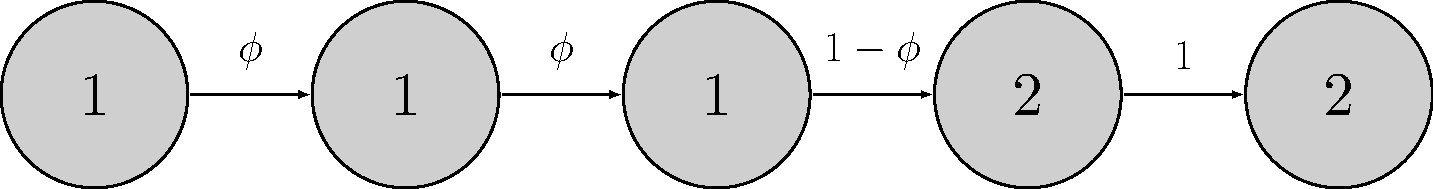
\includegraphics{banana-book_files/figure-latex/unnamed-chunk-12-1.pdf}

Note that the states (in gray) and the observations (in white) do not change. We still have \(z = 1\) for alive, \(z = 2\) for dead, \(y = 1\) for non-detected, and \(y = 2\) for detected.

Parameters are now indexed by time. The survival probability is defined as the probability of staying alive (or ``ah, ha, ha, ha, stayin' alive'' like the Bee Gees would say) over the interval between \(t\) and \(t+1\), that is \(\phi_t = \Pr(z_{t+1} = 1 | z_t = 1)\). The detection probability is defined as the probability of being observed at \(t\) given you're alive at \(t\), that is \(p_t = \Pr(y_{t} = 1 | z_t = 1)\). It is important to bear in mind that survival operates over an interval while detection occurs at a specific time (see Section \ref{covariates}).

The CJS model is named after three statisticians who each published independently a paper introducing more or less the same approach, a year apart ! In fact, Richard Cormack and George Jolly were working in the same corridor in Scotland back in the 1960's. They would meet every day at coffee and would play some game together, but never mention work and were not aware of each other's work.

\hypertarget{capture-recapture-data}{%
\section{Capture-recapture data}\label{capture-recapture-data}}

Before we turn to fitting the CJS model to actual data, let's talk about capture-recapture for a minute. We said in Section \ref{capturerecapturedata} that animals are individually marked. This can be accomplished in two ways, either with artificial marks like rings for birds or ear tags for mammals, or (non-invasive) natural marks like coat patterns or feces DNA sequencing (Figure \ref{fig:marking}).

\begin{figure}
\subfloat[ring\label{fig:marking-1}]{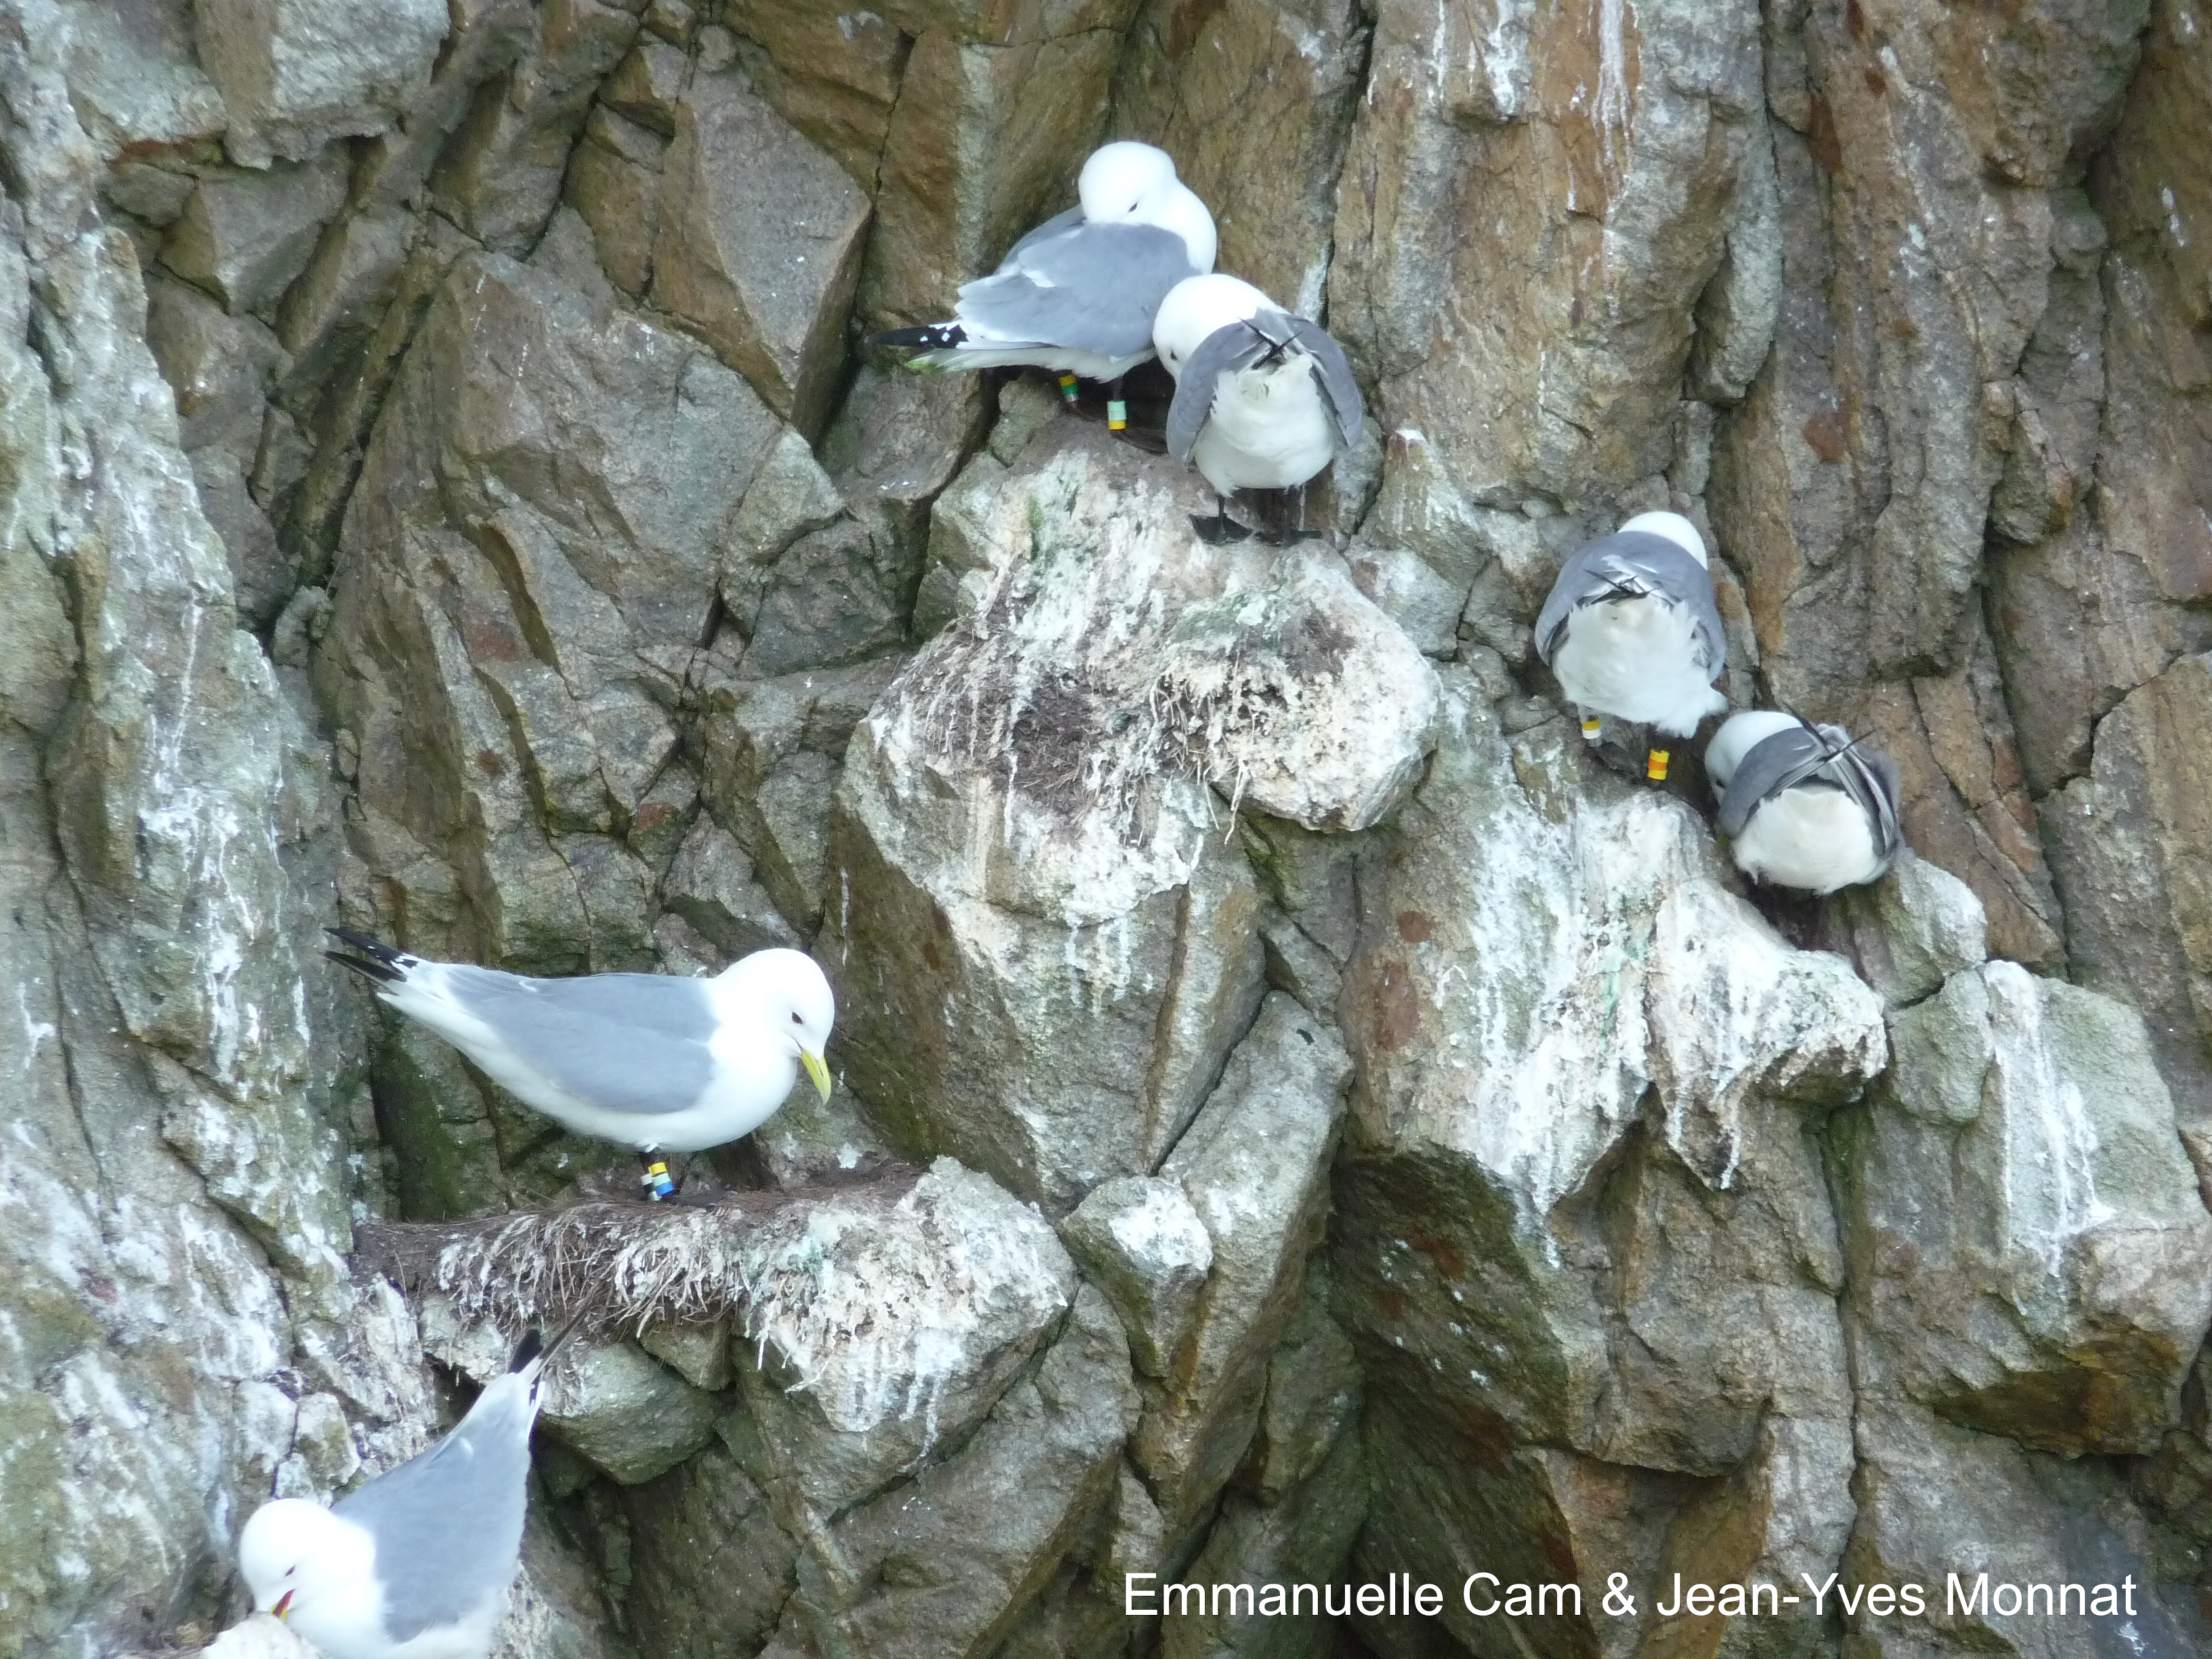
\includegraphics[width=0.5\linewidth]{images/gull} }\subfloat[ear-tag\label{fig:marking-2}]{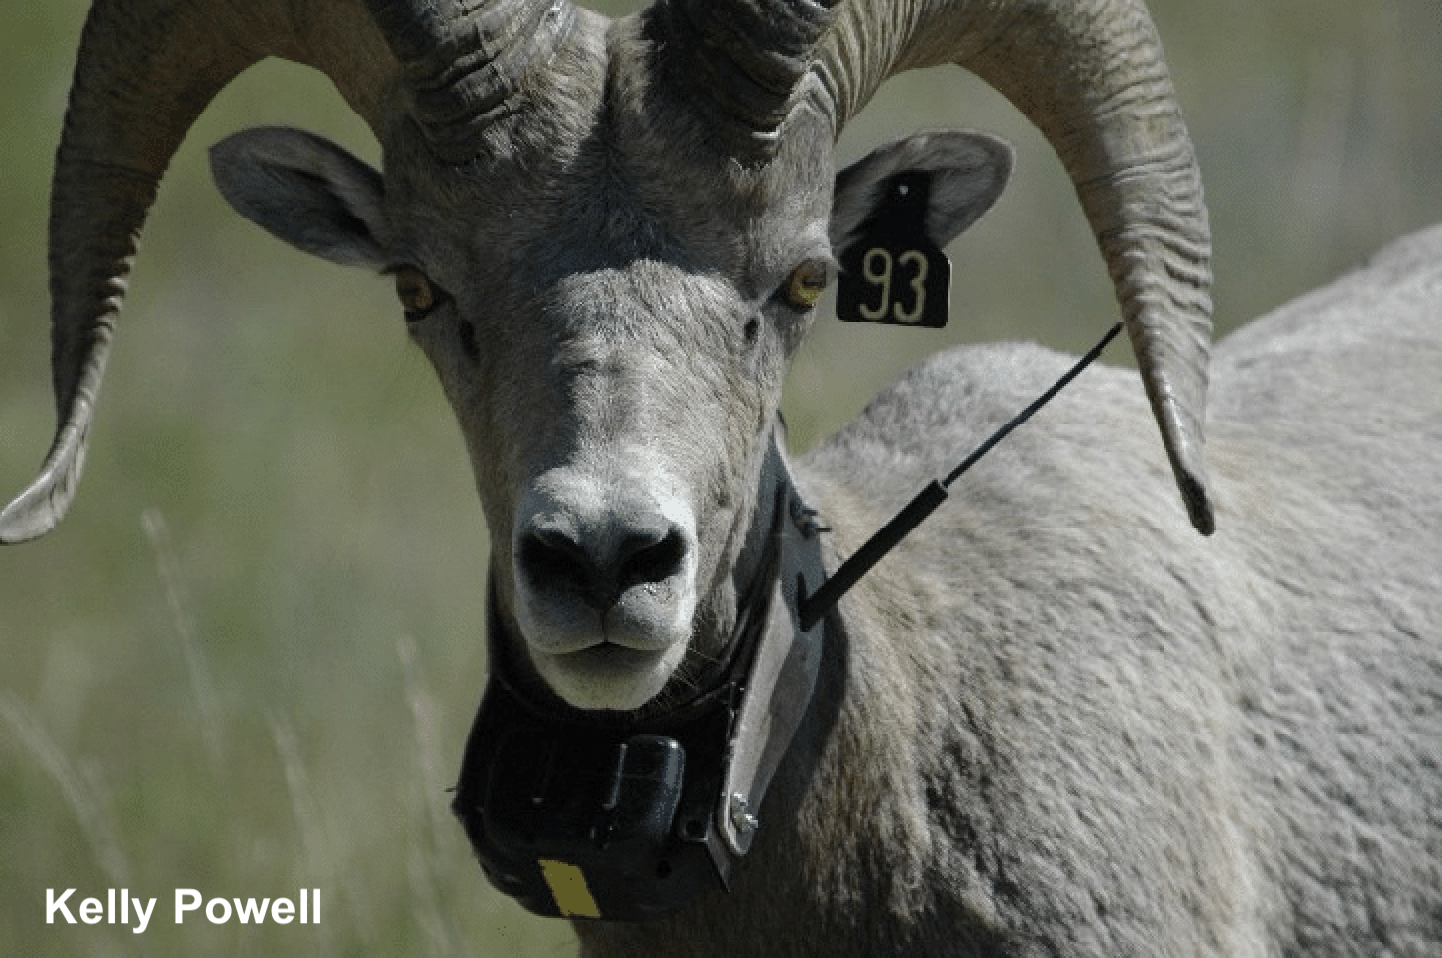
\includegraphics[width=0.5\linewidth]{images/bighorn} }\newline\subfloat[coat patters\label{fig:marking-3}]{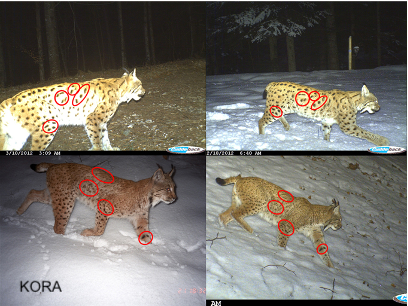
\includegraphics[width=0.5\linewidth]{images/lynx} }\subfloat[ADN feces\label{fig:marking-4}]{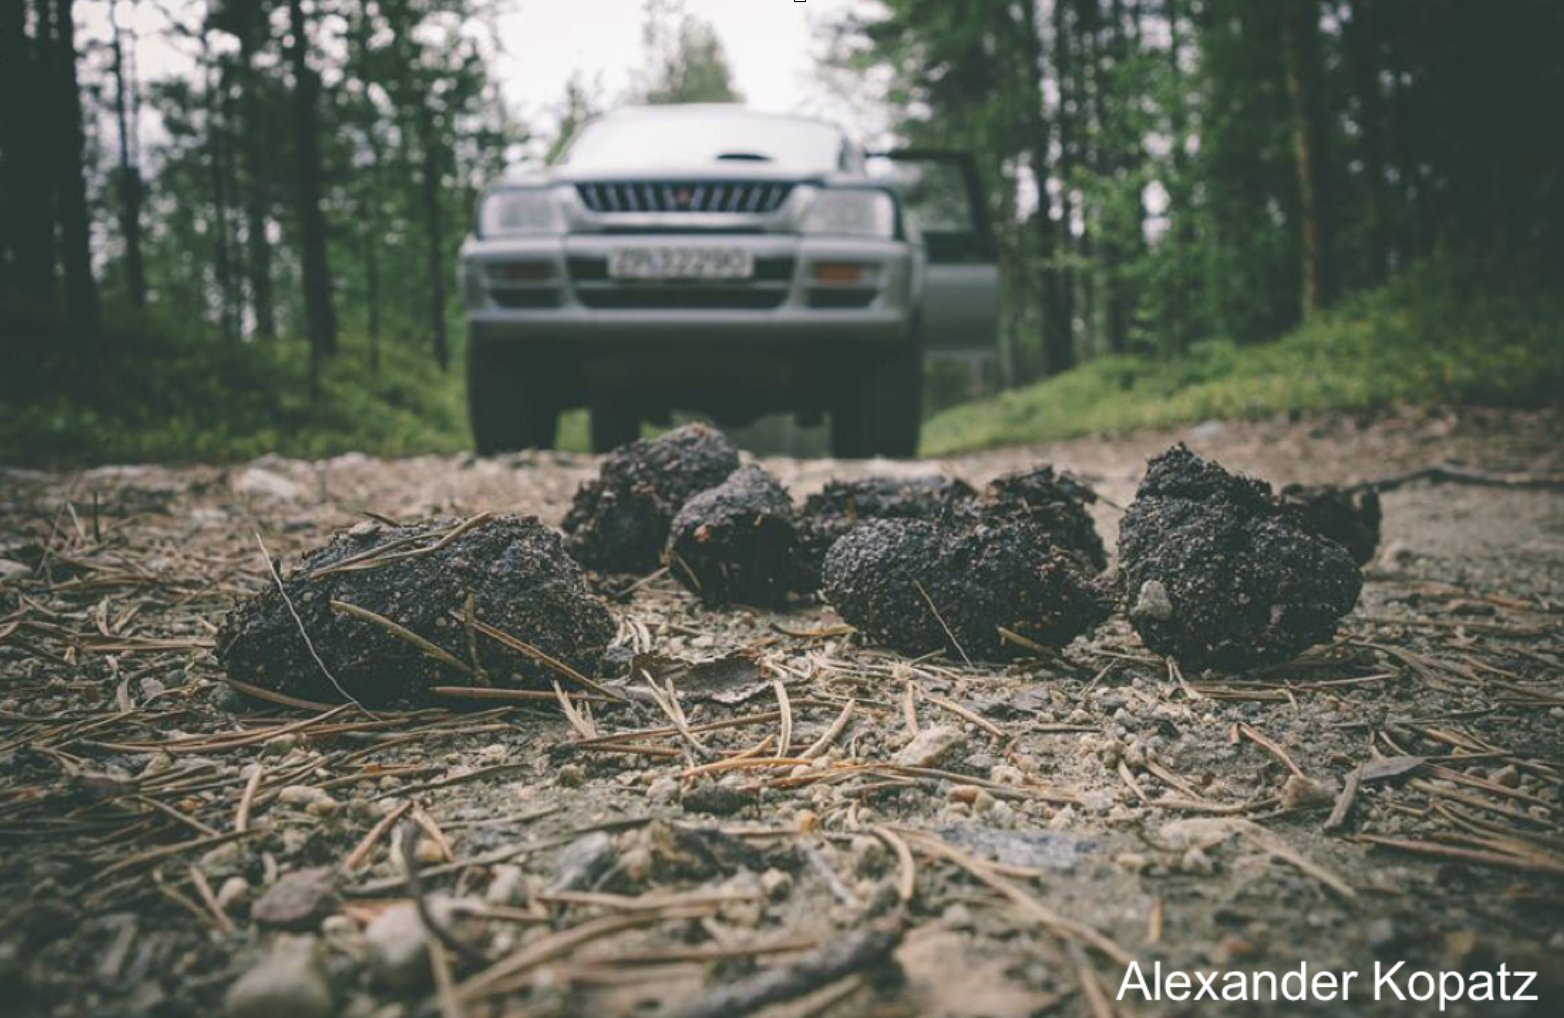
\includegraphics[width=0.5\linewidth]{images/bearscat} }\caption{Animal individual marking. Top-left: rings; Top-right: ear-tags; Bottom left: coat patterns; Bottom right: ADN feces}\label{fig:marking}
\end{figure}

Throughout this chapter, we will use data on the White-throated Dipper (\emph{Cinclus cinclus}; dipper hereafter) kindly provided by Gilbert Marzolin (Figure \ref{fig:pixdipper}). In total, 294 dippers with known sex and wing length were captured and recaptured between 1981 and 1987 during the March-June period. Birds were at least 1 year old when initially banded.

\begin{figure}

{\centering 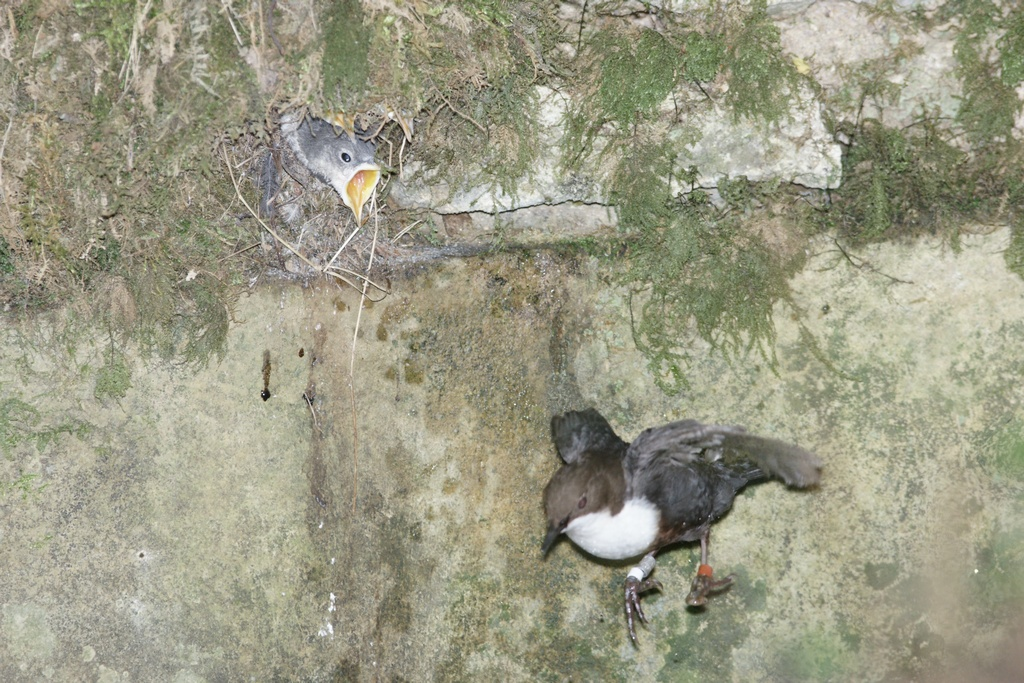
\includegraphics[width=0.6\linewidth]{images/Marzo_BaguesMance} 

}

\caption{White-throated Dipper (Cinclus cinclus)}\label{fig:pixdipper}
\end{figure}

You may scroll down the data below:

The first seven columns are years in which Gilbert went on the field and captured the birds. A 0 stands for a non-detection, and a 1 for a detection. The eighth column informs on the sex of the bird, with F for female and M for male. The last column gives a measure wing length the first time a bird was captured.

\hypertarget{fitting-the-cjs-model-to-the-dipper-data-with-nimble}{%
\section{Fitting the CJS model to the dipper data with NIMBLE}\label{fitting-the-cjs-model-to-the-dipper-data-with-nimble}}

To write the NIMBLE code corresponding to the CJS model, we only need to make a few adjustments to the NIMBLE code for the model with constant parameters from Section \ref{fittinghmmnimble}. The main modification concerns the observation and transition matrices which we need to make time-varying. These matrices therefore become arrays and inherit a third dimension besides that for rows and columns. Also we need priors for all time-varying survival and detection probabilities. We write:

\begin{Shaded}
\begin{Highlighting}[]
\NormalTok{...}
\CommentTok{\# parameters}
\NormalTok{  delta[}\DecValTok{1}\NormalTok{] }\OtherTok{\textless{}{-}} \DecValTok{1}          \CommentTok{\# Pr(alive t = 1) = 1}
\NormalTok{  delta[}\DecValTok{2}\NormalTok{] }\OtherTok{\textless{}{-}} \DecValTok{0}          \CommentTok{\# Pr(dead t = 1) = 0}
  \ControlFlowTok{for}\NormalTok{ (t }\ControlFlowTok{in} \DecValTok{1}\SpecialCharTok{:}\NormalTok{(T}\DecValTok{{-}1}\NormalTok{))\{}
\NormalTok{    phi[t] }\SpecialCharTok{\textasciitilde{}} \FunctionTok{dunif}\NormalTok{(}\DecValTok{0}\NormalTok{, }\DecValTok{1}\NormalTok{) }\CommentTok{\# prior survival}
\NormalTok{    gamma[}\DecValTok{1}\NormalTok{,}\DecValTok{1}\NormalTok{,t] }\OtherTok{\textless{}{-}}\NormalTok{ phi[t]      }\CommentTok{\# Pr(alive t {-}\textgreater{} alive t+1)}
\NormalTok{    gamma[}\DecValTok{1}\NormalTok{,}\DecValTok{2}\NormalTok{,t] }\OtherTok{\textless{}{-}} \DecValTok{1} \SpecialCharTok{{-}}\NormalTok{ phi[t]  }\CommentTok{\# Pr(alive t {-}\textgreater{} dead t+1)}
\NormalTok{    gamma[}\DecValTok{2}\NormalTok{,}\DecValTok{1}\NormalTok{,t] }\OtherTok{\textless{}{-}} \DecValTok{0}        \CommentTok{\# Pr(dead t {-}\textgreater{} alive t+1)}
\NormalTok{    gamma[}\DecValTok{2}\NormalTok{,}\DecValTok{2}\NormalTok{,t] }\OtherTok{\textless{}{-}} \DecValTok{1}        \CommentTok{\# Pr(dead t {-}\textgreater{} dead t+1)}
\NormalTok{    p[t] }\SpecialCharTok{\textasciitilde{}} \FunctionTok{dunif}\NormalTok{(}\DecValTok{0}\NormalTok{, }\DecValTok{1}\NormalTok{) }\CommentTok{\# prior detection}
\NormalTok{    omega[}\DecValTok{1}\NormalTok{,}\DecValTok{1}\NormalTok{,t] }\OtherTok{\textless{}{-}} \DecValTok{1} \SpecialCharTok{{-}}\NormalTok{ p[t]    }\CommentTok{\# Pr(alive t {-}\textgreater{} non{-}detected t)}
\NormalTok{    omega[}\DecValTok{1}\NormalTok{,}\DecValTok{2}\NormalTok{,t] }\OtherTok{\textless{}{-}}\NormalTok{ p[t]        }\CommentTok{\# Pr(alive t {-}\textgreater{} detected t)}
\NormalTok{    omega[}\DecValTok{2}\NormalTok{,}\DecValTok{1}\NormalTok{,t] }\OtherTok{\textless{}{-}} \DecValTok{1}        \CommentTok{\# Pr(dead t {-}\textgreater{} non{-}detected t)}
\NormalTok{    omega[}\DecValTok{2}\NormalTok{,}\DecValTok{2}\NormalTok{,t] }\OtherTok{\textless{}{-}} \DecValTok{0}        \CommentTok{\# Pr(dead t {-}\textgreater{} detected t)}
\NormalTok{  \}}
\NormalTok{...}
\end{Highlighting}
\end{Shaded}

The likelihood does not change, except that the time-varying observation and transition matrices need to be used appropriately. Also, because we now deal with several cohorts of animals first captured, marked and released each year (in contrast with a single cohort as in Chapter \ref{hmmcapturerecapture}), we need to start the loop over time from the first capture for each individual. Therefore, we write:

\begin{Shaded}
\begin{Highlighting}[]
\NormalTok{...}
\CommentTok{\# likelihood}
  \ControlFlowTok{for}\NormalTok{ (i }\ControlFlowTok{in} \DecValTok{1}\SpecialCharTok{:}\NormalTok{N)\{}
\NormalTok{    z[i,first[i]] }\SpecialCharTok{\textasciitilde{}} \FunctionTok{dcat}\NormalTok{(delta[}\DecValTok{1}\SpecialCharTok{:}\DecValTok{2}\NormalTok{])}
    \ControlFlowTok{for}\NormalTok{ (j }\ControlFlowTok{in}\NormalTok{ (first[i]}\SpecialCharTok{+}\DecValTok{1}\NormalTok{)}\SpecialCharTok{:}\NormalTok{T)\{}
\NormalTok{      z[i,j] }\SpecialCharTok{\textasciitilde{}} \FunctionTok{dcat}\NormalTok{(gamma[z[i,j}\DecValTok{{-}1}\NormalTok{], }\DecValTok{1}\SpecialCharTok{:}\DecValTok{2}\NormalTok{, j}\DecValTok{{-}1}\NormalTok{])}
\NormalTok{      y[i,j] }\SpecialCharTok{\textasciitilde{}} \FunctionTok{dcat}\NormalTok{(omega[z[i,j], }\DecValTok{1}\SpecialCharTok{:}\DecValTok{2}\NormalTok{, j}\DecValTok{{-}1}\NormalTok{])}
\NormalTok{    \}}
\NormalTok{  \}}
\NormalTok{...}
\end{Highlighting}
\end{Shaded}

Overall, the code looks like:

\begin{Shaded}
\begin{Highlighting}[]
\NormalTok{hmm.phitpt }\OtherTok{\textless{}{-}} \FunctionTok{nimbleCode}\NormalTok{(\{}
  \CommentTok{\# parameters}
\NormalTok{  delta[}\DecValTok{1}\NormalTok{] }\OtherTok{\textless{}{-}} \DecValTok{1}          \CommentTok{\# Pr(alive t = 1) = 1}
\NormalTok{  delta[}\DecValTok{2}\NormalTok{] }\OtherTok{\textless{}{-}} \DecValTok{0}          \CommentTok{\# Pr(dead t = 1) = 0}
  \ControlFlowTok{for}\NormalTok{ (t }\ControlFlowTok{in} \DecValTok{1}\SpecialCharTok{:}\NormalTok{(T}\DecValTok{{-}1}\NormalTok{))\{}
\NormalTok{    phi[t] }\SpecialCharTok{\textasciitilde{}} \FunctionTok{dunif}\NormalTok{(}\DecValTok{0}\NormalTok{, }\DecValTok{1}\NormalTok{) }\CommentTok{\# prior survival}
\NormalTok{    gamma[}\DecValTok{1}\NormalTok{,}\DecValTok{1}\NormalTok{,t] }\OtherTok{\textless{}{-}}\NormalTok{ phi[t]      }\CommentTok{\# Pr(alive t {-}\textgreater{} alive t+1)}
\NormalTok{    gamma[}\DecValTok{1}\NormalTok{,}\DecValTok{2}\NormalTok{,t] }\OtherTok{\textless{}{-}} \DecValTok{1} \SpecialCharTok{{-}}\NormalTok{ phi[t]  }\CommentTok{\# Pr(alive t {-}\textgreater{} dead t+1)}
\NormalTok{    gamma[}\DecValTok{2}\NormalTok{,}\DecValTok{1}\NormalTok{,t] }\OtherTok{\textless{}{-}} \DecValTok{0}        \CommentTok{\# Pr(dead t {-}\textgreater{} alive t+1)}
\NormalTok{    gamma[}\DecValTok{2}\NormalTok{,}\DecValTok{2}\NormalTok{,t] }\OtherTok{\textless{}{-}} \DecValTok{1}        \CommentTok{\# Pr(dead t {-}\textgreater{} dead t+1)}
\NormalTok{    p[t] }\SpecialCharTok{\textasciitilde{}} \FunctionTok{dunif}\NormalTok{(}\DecValTok{0}\NormalTok{, }\DecValTok{1}\NormalTok{) }\CommentTok{\# prior detection}
\NormalTok{    omega[}\DecValTok{1}\NormalTok{,}\DecValTok{1}\NormalTok{,t] }\OtherTok{\textless{}{-}} \DecValTok{1} \SpecialCharTok{{-}}\NormalTok{ p[t]    }\CommentTok{\# Pr(alive t {-}\textgreater{} non{-}detected t)}
\NormalTok{    omega[}\DecValTok{1}\NormalTok{,}\DecValTok{2}\NormalTok{,t] }\OtherTok{\textless{}{-}}\NormalTok{ p[t]        }\CommentTok{\# Pr(alive t {-}\textgreater{} detected t)}
\NormalTok{    omega[}\DecValTok{2}\NormalTok{,}\DecValTok{1}\NormalTok{,t] }\OtherTok{\textless{}{-}} \DecValTok{1}        \CommentTok{\# Pr(dead t {-}\textgreater{} non{-}detected t)}
\NormalTok{    omega[}\DecValTok{2}\NormalTok{,}\DecValTok{2}\NormalTok{,t] }\OtherTok{\textless{}{-}} \DecValTok{0}        \CommentTok{\# Pr(dead t {-}\textgreater{} detected t)}
\NormalTok{  \}}
  \CommentTok{\# likelihood}
  \ControlFlowTok{for}\NormalTok{ (i }\ControlFlowTok{in} \DecValTok{1}\SpecialCharTok{:}\NormalTok{N)\{}
\NormalTok{    z[i,first[i]] }\SpecialCharTok{\textasciitilde{}} \FunctionTok{dcat}\NormalTok{(delta[}\DecValTok{1}\SpecialCharTok{:}\DecValTok{2}\NormalTok{])}
    \ControlFlowTok{for}\NormalTok{ (j }\ControlFlowTok{in}\NormalTok{ (first[i]}\SpecialCharTok{+}\DecValTok{1}\NormalTok{)}\SpecialCharTok{:}\NormalTok{T)\{}
\NormalTok{      z[i,j] }\SpecialCharTok{\textasciitilde{}} \FunctionTok{dcat}\NormalTok{(gamma[z[i,j}\DecValTok{{-}1}\NormalTok{], }\DecValTok{1}\SpecialCharTok{:}\DecValTok{2}\NormalTok{, j}\DecValTok{{-}1}\NormalTok{])}
\NormalTok{      y[i,j] }\SpecialCharTok{\textasciitilde{}} \FunctionTok{dcat}\NormalTok{(omega[z[i,j], }\DecValTok{1}\SpecialCharTok{:}\DecValTok{2}\NormalTok{, j}\DecValTok{{-}1}\NormalTok{])}
\NormalTok{    \}}
\NormalTok{  \}}
\NormalTok{\})}
\end{Highlighting}
\end{Shaded}

We read in the data:

\begin{Shaded}
\begin{Highlighting}[]
\NormalTok{dipper }\OtherTok{\textless{}{-}} \FunctionTok{read\_csv}\NormalTok{(here}\SpecialCharTok{::}\FunctionTok{here}\NormalTok{(}\StringTok{"dat"}\NormalTok{, }\StringTok{"dipper.csv"}\NormalTok{), }\AttributeTok{show\_col\_types =} \ConstantTok{FALSE}\NormalTok{)}
\NormalTok{y }\OtherTok{\textless{}{-}}\NormalTok{ dipper }\SpecialCharTok{\%\textgreater{}\%}
  \FunctionTok{select}\NormalTok{(year\_1981}\SpecialCharTok{:}\NormalTok{year\_1987) }\SpecialCharTok{\%\textgreater{}\%}
  \FunctionTok{as.matrix}\NormalTok{()}
\end{Highlighting}
\end{Shaded}

We get the occasion of first capture for all individuals, by finding the position of detections in the encounter history (\texttt{which(x\ !=0)}), and keeping the first one:

\begin{Shaded}
\begin{Highlighting}[]
\NormalTok{first }\OtherTok{\textless{}{-}} \FunctionTok{apply}\NormalTok{(y, }\DecValTok{1}\NormalTok{, }\ControlFlowTok{function}\NormalTok{(x) }\FunctionTok{min}\NormalTok{(}\FunctionTok{which}\NormalTok{(x }\SpecialCharTok{!=}\DecValTok{0}\NormalTok{)))}
\end{Highlighting}
\end{Shaded}

Now we specify the constants:

\begin{Shaded}
\begin{Highlighting}[]
\NormalTok{my.constants }\OtherTok{\textless{}{-}} \FunctionTok{list}\NormalTok{(}\AttributeTok{N =} \FunctionTok{nrow}\NormalTok{(y),   }\CommentTok{\# number of animals}
                     \AttributeTok{T =} \FunctionTok{ncol}\NormalTok{(y),   }\CommentTok{\# number of sampling occasions}
                     \AttributeTok{first =}\NormalTok{ first) }\CommentTok{\# first capture for all animales}
\NormalTok{my.constants}
\DocumentationTok{\#\# $N}
\DocumentationTok{\#\# [1] 294}
\DocumentationTok{\#\# }
\DocumentationTok{\#\# $T}
\DocumentationTok{\#\# [1] 7}
\DocumentationTok{\#\# }
\DocumentationTok{\#\# $first}
\DocumentationTok{\#\#   [1] 1 1 1 1 1 1 1 1 1 1 1 1 1 1 1 1 1 1 1 1 1 1 2 2 2 2 2}
\DocumentationTok{\#\#  [28] 2 2 2 2 2 2 2 2 2 2 2 2 2 2 2 2 2 2 2 2 2 2 2 2 2 2 2}
\DocumentationTok{\#\#  [55] 2 2 2 2 2 2 2 2 2 2 2 2 2 2 2 2 2 3 3 3 3 3 3 3 3 3 3}
\DocumentationTok{\#\#  [82] 3 3 3 3 3 3 3 3 3 3 3 3 3 3 3 3 3 3 3 3 3 3 3 3 3 3 3}
\DocumentationTok{\#\# [109] 3 3 3 3 3 3 3 3 3 3 3 3 3 3 3 4 4 4 4 4 4 4 4 4 4 4 4}
\DocumentationTok{\#\# [136] 4 4 4 4 4 4 4 4 4 4 4 4 4 4 4 4 4 4 4 4 4 4 4 4 4 4 4}
\DocumentationTok{\#\# [163] 4 4 4 4 4 4 5 5 5 5 5 5 5 5 5 5 5 5 5 5 5 5 5 5 5 5 5}
\DocumentationTok{\#\# [190] 5 5 5 5 5 5 5 5 5 5 5 5 5 5 5 5 5 5 5 5 6 6 6 6 6 6 6}
\DocumentationTok{\#\# [217] 6 6 6 6 6 6 6 6 6 6 6 6 6 6 6 6 6 6 6 6 6 6 6 6 6 6 6}
\DocumentationTok{\#\# [244] 6 6 6 6 6 6 6 6 6 6 6 6 7 7 7 7 7 7 7 7 7 7 7 7 7 7 7}
\DocumentationTok{\#\# [271] 7 7 7 7 7 7 7 7 7 7 7 7 7 7 7 7 7 7 7 7 7 7 7 7}
\end{Highlighting}
\end{Shaded}

Now we put the data in a list. We add 1 to the data to code non-detections as 1's detections as 2's (see Section @ref\{fittinghmmnimble\}).

\begin{Shaded}
\begin{Highlighting}[]
\NormalTok{my.data }\OtherTok{\textless{}{-}} \FunctionTok{list}\NormalTok{(}\AttributeTok{y =}\NormalTok{ y }\SpecialCharTok{+} \DecValTok{1}\NormalTok{)}
\end{Highlighting}
\end{Shaded}

Now let's write a function for the initial values. For the latent states, we go the easy way, and say that all individuals are alive through the study period:

\begin{Shaded}
\begin{Highlighting}[]
\NormalTok{zinits }\OtherTok{\textless{}{-}}\NormalTok{ y }\SpecialCharTok{+} \DecValTok{1} \CommentTok{\# non{-}detection {-}\textgreater{} alive}
\NormalTok{zinits[zinits }\SpecialCharTok{==} \DecValTok{2}\NormalTok{] }\OtherTok{\textless{}{-}} \DecValTok{1} \CommentTok{\# dead {-}\textgreater{} alive}
\NormalTok{initial.values }\OtherTok{\textless{}{-}} \ControlFlowTok{function}\NormalTok{() }\FunctionTok{list}\NormalTok{(}\AttributeTok{phi =} \FunctionTok{runif}\NormalTok{(my.constants}\SpecialCharTok{$}\NormalTok{T}\DecValTok{{-}1}\NormalTok{,}\DecValTok{0}\NormalTok{,}\DecValTok{1}\NormalTok{),}
                                  \AttributeTok{p =} \FunctionTok{runif}\NormalTok{(my.constants}\SpecialCharTok{$}\NormalTok{T}\DecValTok{{-}1}\NormalTok{,}\DecValTok{0}\NormalTok{,}\DecValTok{1}\NormalTok{),}
                                  \AttributeTok{z =}\NormalTok{ zinits)}
\end{Highlighting}
\end{Shaded}

We specify the parameters we would like to monitor:

\begin{Shaded}
\begin{Highlighting}[]
\NormalTok{parameters.to.save }\OtherTok{\textless{}{-}} \FunctionTok{c}\NormalTok{(}\StringTok{"phi"}\NormalTok{, }\StringTok{"p"}\NormalTok{)}
\end{Highlighting}
\end{Shaded}

We provide MCMC details:

\begin{Shaded}
\begin{Highlighting}[]
\NormalTok{n.iter }\OtherTok{\textless{}{-}} \DecValTok{5000}
\NormalTok{n.burnin }\OtherTok{\textless{}{-}} \DecValTok{1000}
\NormalTok{n.chains }\OtherTok{\textless{}{-}} \DecValTok{2}
\end{Highlighting}
\end{Shaded}

Now we are ready to run NIMBLE:

\begin{Shaded}
\begin{Highlighting}[]
\NormalTok{mcmc.output }\OtherTok{\textless{}{-}} \FunctionTok{nimbleMCMC}\NormalTok{(}\AttributeTok{code =}\NormalTok{ hmm.phitpt,}
                          \AttributeTok{constants =}\NormalTok{ my.constants,}
                          \AttributeTok{data =}\NormalTok{ my.data,}
                          \AttributeTok{inits =}\NormalTok{ initial.values,}
                          \AttributeTok{monitors =}\NormalTok{ parameters.to.save,}
                          \AttributeTok{niter =}\NormalTok{ n.iter,}
                          \AttributeTok{nburnin =}\NormalTok{ n.burnin,}
                          \AttributeTok{nchains =}\NormalTok{ n.chains)}
\end{Highlighting}
\end{Shaded}

We may have a look to the numerical summaries:

\begin{Shaded}
\begin{Highlighting}[]
\FunctionTok{MCMCsummary}\NormalTok{(mcmc.output, }\AttributeTok{round =} \DecValTok{2}\NormalTok{)}
\end{Highlighting}
\end{Shaded}

\begin{verbatim}
##        mean   sd 2.5%  50% 97.5% Rhat n.eff
## phi[1] 0.73 0.14 0.46 0.72  0.99 1.02   199
## phi[2] 0.45 0.07 0.32 0.44  0.59 1.02   410
## phi[3] 0.48 0.06 0.35 0.48  0.59 1.01   506
## phi[4] 0.63 0.06 0.52 0.63  0.75 1.03   415
## phi[5] 0.60 0.06 0.49 0.60  0.72 1.01   365
## phi[6] 0.74 0.13 0.51 0.74  0.97 1.10    38
## p[1]   0.66 0.14 0.38 0.67  0.89 1.01   344
## p[2]   0.87 0.08 0.68 0.89  0.98 1.02   249
## p[3]   0.88 0.07 0.73 0.89  0.97 1.02   307
## p[4]   0.87 0.06 0.74 0.88  0.96 1.05   333
## p[5]   0.90 0.05 0.77 0.91  0.98 1.01   224
## p[6]   0.72 0.13 0.50 0.72  0.97 1.08    37
\end{verbatim}

There is not so much time variation in the detection probability which is estimated high around 0.90. Note that \texttt{p{[}1{]}} corresponds to the detection probability in 1982 that is \(p_2\), \texttt{p{[}2{]}} to detection in 1983 therefore \(p_3\), and so on. In contrast, the dippers seem to have experienced a decrease in survival in years 1982-1983 (\texttt{phi{[}2{]}}) and 1983-1984 (\texttt{phi{[}4{]}}). We will get back to that in Section \ref{covariates}.

You may have noticed the small effective sample size for the last survival (\texttt{phi{[}6{]}}) and detection (\texttt{p{[}6{]}}) probabilities. Let's have a look to mixing for parameter \texttt{phi{[}6{]}} for example:

\begin{Shaded}
\begin{Highlighting}[]
\NormalTok{priors }\OtherTok{\textless{}{-}} \FunctionTok{runif}\NormalTok{(}\DecValTok{3000}\NormalTok{, }\DecValTok{0}\NormalTok{, }\DecValTok{1}\NormalTok{)}
\FunctionTok{MCMCtrace}\NormalTok{(}\AttributeTok{object =}\NormalTok{ mcmc.phitpt,}
          \AttributeTok{ISB =} \ConstantTok{FALSE}\NormalTok{,}
          \AttributeTok{exact =} \ConstantTok{TRUE}\NormalTok{, }
          \AttributeTok{params =} \FunctionTok{c}\NormalTok{(}\StringTok{"phi[6]"}\NormalTok{),}
          \AttributeTok{pdf =} \ConstantTok{FALSE}\NormalTok{, }
          \AttributeTok{priors =}\NormalTok{ priors)}
\end{Highlighting}
\end{Shaded}

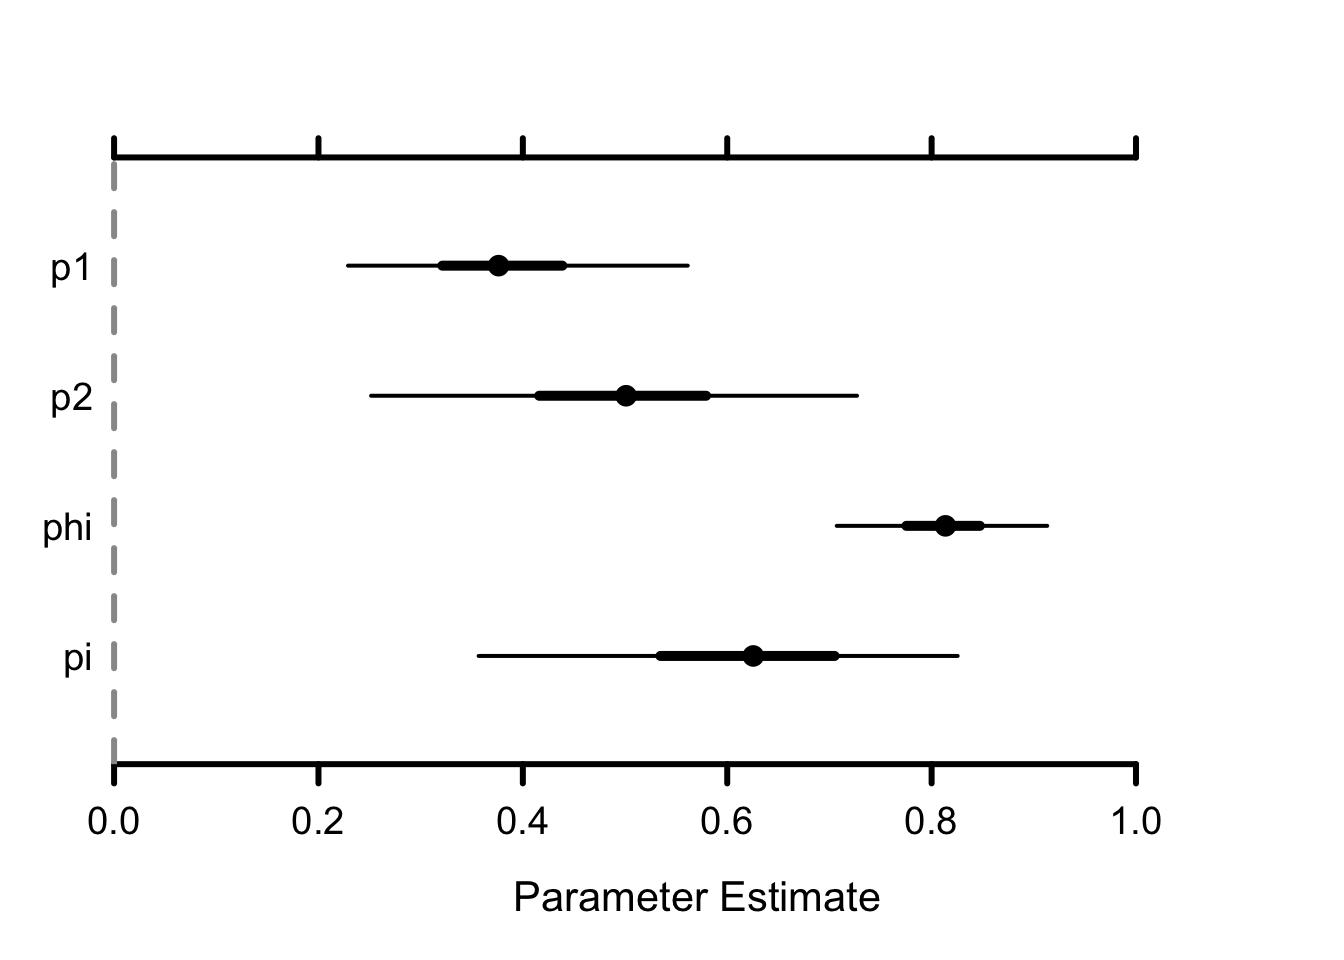
\includegraphics{banana-book_files/figure-latex/unnamed-chunk-27-1.pdf}

Clearly mixing (left panel in the plot above) is bad and there is a big overlap between the prior and the posterior for this parameter (right panel) suggesting that its prior was not well updated with the data. What is going on? If you could inspect the likelihood of the CJS model, you would realise that these two parameters \(\phi_6\) and \(p_7\) appear only as the product \(\phi_6 p_7\) and cannot be estimated separately. In other words, one of these parameters is redundant, and you'd need an extra sampling occasion to be able to disentangle them. This is not a big issue as long as you're aware of it and you do not attempt to ecologically interpret these parameters.

\hypertarget{cjs-model-derivatives}{%
\section{CJS model derivatives}\label{cjs-model-derivatives}}

Besides the model we considered with constant parameters (see Chapter \ref{hmmcapturerecapture}) and the CJS model with time-varying parameters, you might want to fit in-between or models with time variation on either detection or survival.

Let's start with the model with time-varying survival and constant detection. We modify the CJS model NIMBLE code by no longer having the observation matrix time-specific:

\begin{Shaded}
\begin{Highlighting}[]
\NormalTok{hmm.phitp }\OtherTok{\textless{}{-}} \FunctionTok{nimbleCode}\NormalTok{(\{}
  \ControlFlowTok{for}\NormalTok{ (t }\ControlFlowTok{in} \DecValTok{1}\SpecialCharTok{:}\NormalTok{(T}\DecValTok{{-}1}\NormalTok{))\{}
\NormalTok{    phi[t] }\SpecialCharTok{\textasciitilde{}} \FunctionTok{dunif}\NormalTok{(}\DecValTok{0}\NormalTok{, }\DecValTok{1}\NormalTok{) }\CommentTok{\# prior survival}
\NormalTok{    gamma[}\DecValTok{1}\NormalTok{,}\DecValTok{1}\NormalTok{,t] }\OtherTok{\textless{}{-}}\NormalTok{ phi[t]      }\CommentTok{\# Pr(alive t {-}\textgreater{} alive t+1)}
\NormalTok{    gamma[}\DecValTok{1}\NormalTok{,}\DecValTok{2}\NormalTok{,t] }\OtherTok{\textless{}{-}} \DecValTok{1} \SpecialCharTok{{-}}\NormalTok{ phi[t]  }\CommentTok{\# Pr(alive t {-}\textgreater{} dead t+1)}
\NormalTok{    gamma[}\DecValTok{2}\NormalTok{,}\DecValTok{1}\NormalTok{,t] }\OtherTok{\textless{}{-}} \DecValTok{0}        \CommentTok{\# Pr(dead t {-}\textgreater{} alive t+1)}
\NormalTok{    gamma[}\DecValTok{2}\NormalTok{,}\DecValTok{2}\NormalTok{,t] }\OtherTok{\textless{}{-}} \DecValTok{1}        \CommentTok{\# Pr(dead t {-}\textgreater{} dead t+1)}
\NormalTok{  \}}
\NormalTok{  p }\SpecialCharTok{\textasciitilde{}} \FunctionTok{dunif}\NormalTok{(}\DecValTok{0}\NormalTok{, }\DecValTok{1}\NormalTok{) }\CommentTok{\# prior detection}
\NormalTok{  delta[}\DecValTok{1}\NormalTok{] }\OtherTok{\textless{}{-}} \DecValTok{1}          \CommentTok{\# Pr(alive t = 1) = 1}
\NormalTok{  delta[}\DecValTok{2}\NormalTok{] }\OtherTok{\textless{}{-}} \DecValTok{0}          \CommentTok{\# Pr(dead t = 1) = 0}
\NormalTok{  omega[}\DecValTok{1}\NormalTok{,}\DecValTok{1}\NormalTok{] }\OtherTok{\textless{}{-}} \DecValTok{1} \SpecialCharTok{{-}}\NormalTok{ p    }\CommentTok{\# Pr(alive t {-}\textgreater{} non{-}detected t)}
\NormalTok{  omega[}\DecValTok{1}\NormalTok{,}\DecValTok{2}\NormalTok{] }\OtherTok{\textless{}{-}}\NormalTok{ p        }\CommentTok{\# Pr(alive t {-}\textgreater{} detected t)}
\NormalTok{  omega[}\DecValTok{2}\NormalTok{,}\DecValTok{1}\NormalTok{] }\OtherTok{\textless{}{-}} \DecValTok{1}        \CommentTok{\# Pr(dead t {-}\textgreater{} non{-}detected t)}
\NormalTok{  omega[}\DecValTok{2}\NormalTok{,}\DecValTok{2}\NormalTok{] }\OtherTok{\textless{}{-}} \DecValTok{0}        \CommentTok{\# Pr(dead t {-}\textgreater{} detected t)}
  \CommentTok{\# likelihood}
  \ControlFlowTok{for}\NormalTok{ (i }\ControlFlowTok{in} \DecValTok{1}\SpecialCharTok{:}\NormalTok{N)\{}
\NormalTok{    z[i,first[i]] }\SpecialCharTok{\textasciitilde{}} \FunctionTok{dcat}\NormalTok{(delta[}\DecValTok{1}\SpecialCharTok{:}\DecValTok{2}\NormalTok{])}
    \ControlFlowTok{for}\NormalTok{ (j }\ControlFlowTok{in}\NormalTok{ (first[i]}\SpecialCharTok{+}\DecValTok{1}\NormalTok{)}\SpecialCharTok{:}\NormalTok{T)\{}
\NormalTok{      z[i,j] }\SpecialCharTok{\textasciitilde{}} \FunctionTok{dcat}\NormalTok{(gamma[z[i,j}\DecValTok{{-}1}\NormalTok{], }\DecValTok{1}\SpecialCharTok{:}\DecValTok{2}\NormalTok{, j}\DecValTok{{-}1}\NormalTok{])}
\NormalTok{      y[i,j] }\SpecialCharTok{\textasciitilde{}} \FunctionTok{dcat}\NormalTok{(omega[z[i,j], }\DecValTok{1}\SpecialCharTok{:}\DecValTok{2}\NormalTok{])}
\NormalTok{    \}}
\NormalTok{  \}}
\NormalTok{\})}
\end{Highlighting}
\end{Shaded}

We obtain the following numerical summaries for parameters, confirming high detection and temporal variation in survival:

\begin{verbatim}
##        mean   sd 2.5%  50% 97.5% Rhat n.eff
## phi[1] 0.63 0.10 0.42 0.63  0.82 1.04   564
## phi[2] 0.46 0.06 0.35 0.46  0.59 1.01   629
## phi[3] 0.48 0.05 0.37 0.48  0.59 1.00   610
## phi[4] 0.62 0.06 0.51 0.62  0.73 1.00   553
## phi[5] 0.61 0.05 0.50 0.61  0.72 1.00   568
## phi[6] 0.59 0.05 0.48 0.59  0.69 1.03   463
## p      0.89 0.03 0.82 0.89  0.95 1.04   211
\end{verbatim}

Now the model with time-varying detection and constant survival, for which the NIMBLE code has a constant over time transition matrix:

\begin{Shaded}
\begin{Highlighting}[]
\NormalTok{hmm.phipt }\OtherTok{\textless{}{-}} \FunctionTok{nimbleCode}\NormalTok{(\{}
\NormalTok{  phi }\SpecialCharTok{\textasciitilde{}} \FunctionTok{dunif}\NormalTok{(}\DecValTok{0}\NormalTok{, }\DecValTok{1}\NormalTok{) }\CommentTok{\# prior survival}
\NormalTok{  gamma[}\DecValTok{1}\NormalTok{,}\DecValTok{1}\NormalTok{] }\OtherTok{\textless{}{-}}\NormalTok{ phi      }\CommentTok{\# Pr(alive t {-}\textgreater{} alive t+1)}
\NormalTok{  gamma[}\DecValTok{1}\NormalTok{,}\DecValTok{2}\NormalTok{] }\OtherTok{\textless{}{-}} \DecValTok{1} \SpecialCharTok{{-}}\NormalTok{ phi  }\CommentTok{\# Pr(alive t {-}\textgreater{} dead t+1)}
\NormalTok{  gamma[}\DecValTok{2}\NormalTok{,}\DecValTok{1}\NormalTok{] }\OtherTok{\textless{}{-}} \DecValTok{0}        \CommentTok{\# Pr(dead t {-}\textgreater{} alive t+1)}
\NormalTok{  gamma[}\DecValTok{2}\NormalTok{,}\DecValTok{2}\NormalTok{] }\OtherTok{\textless{}{-}} \DecValTok{1}        \CommentTok{\# Pr(dead t {-}\textgreater{} dead t+1)}
\NormalTok{  delta[}\DecValTok{1}\NormalTok{] }\OtherTok{\textless{}{-}} \DecValTok{1}          \CommentTok{\# Pr(alive t = 1) = 1}
\NormalTok{  delta[}\DecValTok{2}\NormalTok{] }\OtherTok{\textless{}{-}} \DecValTok{0}          \CommentTok{\# Pr(dead t = 1) = 0}
  \ControlFlowTok{for}\NormalTok{ (t }\ControlFlowTok{in} \DecValTok{1}\SpecialCharTok{:}\NormalTok{(T}\DecValTok{{-}1}\NormalTok{))\{}
\NormalTok{    p[t] }\SpecialCharTok{\textasciitilde{}} \FunctionTok{dunif}\NormalTok{(}\DecValTok{0}\NormalTok{, }\DecValTok{1}\NormalTok{) }\CommentTok{\# prior detection}
\NormalTok{    omega[}\DecValTok{1}\NormalTok{,}\DecValTok{1}\NormalTok{,t] }\OtherTok{\textless{}{-}} \DecValTok{1} \SpecialCharTok{{-}}\NormalTok{ p[t]    }\CommentTok{\# Pr(alive t {-}\textgreater{} non{-}detected t)}
\NormalTok{    omega[}\DecValTok{1}\NormalTok{,}\DecValTok{2}\NormalTok{,t] }\OtherTok{\textless{}{-}}\NormalTok{ p[t]        }\CommentTok{\# Pr(alive t {-}\textgreater{} detected t)}
\NormalTok{    omega[}\DecValTok{2}\NormalTok{,}\DecValTok{1}\NormalTok{,t] }\OtherTok{\textless{}{-}} \DecValTok{1}        \CommentTok{\# Pr(dead t {-}\textgreater{} non{-}detected t)}
\NormalTok{    omega[}\DecValTok{2}\NormalTok{,}\DecValTok{2}\NormalTok{,t] }\OtherTok{\textless{}{-}} \DecValTok{0}        \CommentTok{\# Pr(dead t {-}\textgreater{} detected t)}
\NormalTok{  \}}
  \CommentTok{\# likelihood}
  \ControlFlowTok{for}\NormalTok{ (i }\ControlFlowTok{in} \DecValTok{1}\SpecialCharTok{:}\NormalTok{N)\{}
\NormalTok{    z[i,first[i]] }\SpecialCharTok{\textasciitilde{}} \FunctionTok{dcat}\NormalTok{(delta[}\DecValTok{1}\SpecialCharTok{:}\DecValTok{2}\NormalTok{])}
    \ControlFlowTok{for}\NormalTok{ (j }\ControlFlowTok{in}\NormalTok{ (first[i]}\SpecialCharTok{+}\DecValTok{1}\NormalTok{)}\SpecialCharTok{:}\NormalTok{T)\{}
\NormalTok{      z[i,j] }\SpecialCharTok{\textasciitilde{}} \FunctionTok{dcat}\NormalTok{(gamma[z[i,j}\DecValTok{{-}1}\NormalTok{], }\DecValTok{1}\SpecialCharTok{:}\DecValTok{2}\NormalTok{])}
\NormalTok{      y[i,j] }\SpecialCharTok{\textasciitilde{}} \FunctionTok{dcat}\NormalTok{(omega[z[i,j], }\DecValTok{1}\SpecialCharTok{:}\DecValTok{2}\NormalTok{, j}\DecValTok{{-}1}\NormalTok{])}
\NormalTok{    \}}
\NormalTok{  \}}
\NormalTok{\})}
\end{Highlighting}
\end{Shaded}

Numerical summaries for the parameters are:

\begin{verbatim}
##      mean   sd 2.5%  50% 97.5% Rhat n.eff
## phi  0.56 0.03 0.52 0.56  0.61 1.02   381
## p[1] 0.75 0.12 0.48 0.77  0.93 1.03   452
## p[2] 0.85 0.08 0.68 0.86  0.97 1.02   359
## p[3] 0.85 0.07 0.69 0.85  0.96 1.00   316
## p[4] 0.89 0.05 0.77 0.89  0.97 1.00   412
## p[5] 0.91 0.04 0.82 0.92  0.98 1.00   376
## p[6] 0.90 0.07 0.73 0.91  1.00 1.07   111
\end{verbatim}

We note that these two models do no longer have parameter redundancy issues. We are left with four models, each saying a different story about the data, with temporal variation or not in either survival or detection probabilty. How to quantify the most plausible of these four ecological hypotheses? Rendez-vous in the next section.

\hypertarget{waic}{%
\section{Model comparison with WAIC}\label{waic}}

Which of the four models above is best supported by the data? To answer this question, we need to bear in mind that we used all the observed data to fit these models, and how close to the truth these models will perform when predicting for future data -- or predictive accuracy -- should be assessed. A natural candidate measure for predictive accuracy is the likelihood which is often referred in the context of model comparison as the predictive density. However, we know neither the true process, nor the future data, and we can only estimate the predictive density with some bias.

You may have heard about the Akaike Information Criterion (AIC) in the Frequentist framework, and the Deviance Information Criterion (DIC) in the Bayesian framework. We will consider here the Widely Applicable Information Criterion or Watanabe Information Criterion (WAIC). AIC, DIC and WAIC each aim to provide an approximation of predictive accuracy.

While AIC is the predictive measure of choice in the Frequentist framework for ecologists, DIC has been around for some time for Bayesian applications due to its availability in population BUGS pieces of software. However, these methods only utilize a point estimate of the unknown parameters. Also, various difficulties have been noted with DIC which may give nonsensical results when the posterior distribution is not well summarized by its mean. For a more fully Bayesian approach we would like to use the entire posterior distribution to evaluate the predictive performance, which is exactly what WAIC does.

Conveniently, NIMBLE calculates WAIC for you. The only modifications we need to make are i) to monitor the latent states and ii) to add \texttt{WAIC\ =\ TRUE} in the call to the \texttt{nimbleMCMC()} function. For example, for the CJS model, we would write:

\begin{Shaded}
\begin{Highlighting}[]
\NormalTok{parameters.to.save }\OtherTok{\textless{}{-}} \FunctionTok{c}\NormalTok{(}\StringTok{"phi"}\NormalTok{, }\StringTok{"p"}\NormalTok{, }\StringTok{"z"}\NormalTok{) }
\NormalTok{mcmc.phitpt }\OtherTok{\textless{}{-}} \FunctionTok{nimbleMCMC}\NormalTok{(}\AttributeTok{code =}\NormalTok{ hmm.phitpt,}
                          \AttributeTok{constants =}\NormalTok{ my.constants,}
                          \AttributeTok{data =}\NormalTok{ my.data,}
                          \AttributeTok{inits =}\NormalTok{ initial.values,}
                          \AttributeTok{monitors =}\NormalTok{ parameters.to.save,}
                          \AttributeTok{niter =}\NormalTok{ n.iter,}
                          \AttributeTok{nburnin =}\NormalTok{ n.burnin,}
                          \AttributeTok{nchains =}\NormalTok{ n.chains,}
                          \AttributeTok{WAIC =} \ConstantTok{TRUE}\NormalTok{) }
\end{Highlighting}
\end{Shaded}

I re-ran the four models to calculate the WAIC value for each of them

\begin{verbatim}
##                                                    model
## 1        model with both survival and detection constant
## 2 model with time-dependent survival, constant detection
## 3 model with constant survival, time-dependent detection
## 4                                              CJS model
##    WAIC
## 1 265.9
## 2 277.6
## 3 270.2
## 4 308.8
\end{verbatim}

Lower values of WAIC imply higher predictive accuracy, thefore we would favor model with constant parameters.

\hypertarget{goodness-of-fit-testing}{%
\section{Goodness-of-fit testing}\label{goodness-of-fit-testing}}

In the previous Section \ref{waic}, we compared models between each other based on their predictive accuracy -- we assessed their \emph{relative} fit. However, even though we were able to rank these models according to predictive accuracy, it could happen that all models actually had poor predictive performance -- this has to do with \emph{absolute} fit.

How to assess the goodness of fit of the CJS model to capture-recapture data? In particular how to assess homogeneity of survival and detection probabilities which is a fundamental assumption for this model?

In the Bayesian framework, we would rely on posterior predictive checks to assess absolute fit. Briefly speaking, the idea is to compare the observed data to replicated data generated from the model. If the model is a good fit to the data, then the replicated data predicted from the model should look similar to the observed data. To simplify the comparison, some summary statistics are generally considered that should be built based on the ecological question of interest.

For the CJS model, posterior predictive checks can be used. However, there are well established procedures for assessing absolute fit and departures from specific model assumptions that would be a shame to just ignore.

We focus on two such assumptions that have an ecological interpretation, transience and trap-dependence. The transience procedure assesses whether newly encountered individuals have the same chance to be later re-observed as recaptured (previously encountered) individuals. The trap-dependence procedure assesses whether missed individuals have the same chance to be recaptured at the next occasion as currently captured individuals. Although these procedures are called \emph{test of transience} and \emph{test of trap-dependence}, when it comes to interpretation, you should keep in mind that transience -- an excess of individuals never seen again -- and trap-dependence -- an effect of trapping on detection -- are just two specific reasons why the tests might detect a lack of fit.

These tests are implemented in the package \texttt{R2ucare}, and we illustrate its use with the dipper data.

\begin{Shaded}
\begin{Highlighting}[]
\FunctionTok{library}\NormalTok{(R2ucare)}
\end{Highlighting}
\end{Shaded}

We get the capture-recapture data:

\begin{Shaded}
\begin{Highlighting}[]
\CommentTok{\# capture{-}recapture data}
\NormalTok{dipper }\OtherTok{\textless{}{-}} \FunctionTok{read\_csv}\NormalTok{(here}\SpecialCharTok{::}\FunctionTok{here}\NormalTok{(}\StringTok{"dat"}\NormalTok{, }\StringTok{"dipper.csv"}\NormalTok{))}
\NormalTok{dip.hist }\OtherTok{\textless{}{-}}\NormalTok{ dipper }\SpecialCharTok{\%\textgreater{}\%}
  \FunctionTok{select}\NormalTok{(year\_1981}\SpecialCharTok{:}\NormalTok{year\_1987) }\SpecialCharTok{\%\textgreater{}\%}
  \FunctionTok{as.matrix}\NormalTok{()}
\CommentTok{\# number of birds with that particular capture{-}recapture history}
\NormalTok{dip.freq }\OtherTok{\textless{}{-}} \FunctionTok{rep}\NormalTok{(}\DecValTok{1}\NormalTok{, }\FunctionTok{nrow}\NormalTok{(dip.hist))}
\CommentTok{\# sex of each bird}
\NormalTok{dip.group }\OtherTok{\textless{}{-}}\NormalTok{ dipper}\SpecialCharTok{$}\NormalTok{sex}
\end{Highlighting}
\end{Shaded}

For the sake of illustration, we consider females only:

\begin{Shaded}
\begin{Highlighting}[]
\NormalTok{mask }\OtherTok{\textless{}{-}}\NormalTok{ (dip.group }\SpecialCharTok{==} \StringTok{\textquotesingle{}F\textquotesingle{}}\NormalTok{)}
\NormalTok{dip.fem.hist }\OtherTok{\textless{}{-}}\NormalTok{ dip.hist[mask,]}
\NormalTok{dip.fem.freq }\OtherTok{\textless{}{-}}\NormalTok{ dip.freq[mask]}
\end{Highlighting}
\end{Shaded}

The overall test shows that we cannot reject the hypothesis that the CJS models fits the data well:

\begin{Shaded}
\begin{Highlighting}[]
\FunctionTok{overall\_CJS}\NormalTok{(dip.fem.hist, dip.fem.freq)}
\DocumentationTok{\#\#                          chi2 degree\_of\_freedom p\_value}
\DocumentationTok{\#\# Gof test for CJS model: 10.28                12   0.592}
\end{Highlighting}
\end{Shaded}

We may perform a test specifically to assess a transient effect:

\begin{Shaded}
\begin{Highlighting}[]
\FunctionTok{test3sr}\NormalTok{(dip.fem.hist, dip.fem.freq)}
\DocumentationTok{\#\# $test3sr}
\DocumentationTok{\#\#      stat        df     p\_val sign\_test }
\DocumentationTok{\#\#     4.985     5.000     0.418     1.428 }
\DocumentationTok{\#\# }
\DocumentationTok{\#\# $details}
\DocumentationTok{\#\#   component  stat p\_val signed\_test  test\_perf}
\DocumentationTok{\#\# 1         2 0.858 0.354       0.926 Chi{-}square}
\DocumentationTok{\#\# 2         3 3.586 0.058       1.894 Chi{-}square}
\DocumentationTok{\#\# 3         4 0.437 0.509       0.661 Chi{-}square}
\DocumentationTok{\#\# 4         5 0.103 0.748      {-}0.321 Chi{-}square}
\DocumentationTok{\#\# 5         6 0.001 0.982       0.032 Chi{-}square}
\end{Highlighting}
\end{Shaded}

Or trap-dependence:

\begin{Shaded}
\begin{Highlighting}[]
\FunctionTok{test2ct}\NormalTok{(dip.fem.hist, dip.fem.freq)}
\DocumentationTok{\#\# $test2ct}
\DocumentationTok{\#\#      stat        df     p\_val sign\_test }
\DocumentationTok{\#\#     3.250     4.000     0.517    {-}0.901 }
\DocumentationTok{\#\# }
\DocumentationTok{\#\# $details}
\DocumentationTok{\#\#   component dof stat p\_val signed\_test test\_perf}
\DocumentationTok{\#\# 1         2   1    0     1           0    Fisher}
\DocumentationTok{\#\# 2         3   1    0     1           0    Fisher}
\DocumentationTok{\#\# 3         4   1    0     1           0    Fisher}
\DocumentationTok{\#\# 4         5   1 3.25 0.071      {-}1.803    Fisher}
\end{Highlighting}
\end{Shaded}

\textbf{What to do if these tests are significant? If you detect a transient effect, then 2 age classes should be considered on survival probability to account for this issue (fast forward covariate section below). Explain without talking about age effect, and why it is on survival that the effect should be considered. If trap dependence is significant, you could use a time-varying individual covariate to account for this effect. Explain the covariate (fast forward section on covariate below), or consider more complex models. Explain multievent model without talking about states (fast forward case study).}

So far, we have addressed assumptions relative to the model. There are also assumptions relative to the design. In particular, survival refers to the study area, and so we need to think carefully about what survival does actually mean. We actually estimate what we usually call \emph{apparent} survival, not exactly \emph{true} survival. Apparent survival probability is the product of true survival and study area fidelity. Consequently, apparent survival is always lower than true survival unless study area fidelity is exactly 1. There are other assumptions relative to the design, which we simply list here. There should be no mark loss, the identity of individuals should be recorded without error (no false positives), and captured animals should be a random sample of the population.

\hypertarget{covariates}{%
\section{Covariates}\label{covariates}}

\textbf{Blabla sur le pourquoi des covariables.}

\hypertarget{temporal-covariates}{%
\subsection{Temporal covariates}\label{temporal-covariates}}

\hypertarget{discrete}{%
\subsubsection{Discrete}\label{discrete}}

Also consider flood effect discrete cov. A major flood occurred during the 1983 breeding season. Because captures during the breding season occurred well before and after the flood, survival in the two years 1982-1983 and 1983-1984 were likely to be affected. Indeed survival of a species living along and feeding in the river in these two flood years was most likely lower than in nonflood years.

\begin{Shaded}
\begin{Highlighting}[]
\NormalTok{hmm.phifloodp }\OtherTok{\textless{}{-}} \FunctionTok{nimbleCode}\NormalTok{(\{}
\NormalTok{  delta[}\DecValTok{1}\NormalTok{] }\OtherTok{\textless{}{-}} \DecValTok{1}          \CommentTok{\# Pr(alive t = 1) = 1}
\NormalTok{  delta[}\DecValTok{2}\NormalTok{] }\OtherTok{\textless{}{-}} \DecValTok{0}          \CommentTok{\# Pr(dead t = 1) = 0}
  \ControlFlowTok{for}\NormalTok{ (t }\ControlFlowTok{in} \DecValTok{1}\SpecialCharTok{:}\NormalTok{(T}\DecValTok{{-}1}\NormalTok{))\{}
    \FunctionTok{logit}\NormalTok{(phi[t]) }\OtherTok{\textless{}{-}}\NormalTok{ beta[}\DecValTok{1}\NormalTok{] }\SpecialCharTok{+}\NormalTok{ beta[}\DecValTok{2}\NormalTok{] }\SpecialCharTok{*}\NormalTok{ flood[t]}
\NormalTok{    gamma[}\DecValTok{1}\NormalTok{,}\DecValTok{1}\NormalTok{,t] }\OtherTok{\textless{}{-}}\NormalTok{ phi[t]      }\CommentTok{\# Pr(alive t {-}\textgreater{} alive t+1)}
\NormalTok{    gamma[}\DecValTok{1}\NormalTok{,}\DecValTok{2}\NormalTok{,t] }\OtherTok{\textless{}{-}} \DecValTok{1} \SpecialCharTok{{-}}\NormalTok{ phi[t]  }\CommentTok{\# Pr(alive t {-}\textgreater{} dead t+1)}
\NormalTok{    gamma[}\DecValTok{2}\NormalTok{,}\DecValTok{1}\NormalTok{,t] }\OtherTok{\textless{}{-}} \DecValTok{0}        \CommentTok{\# Pr(dead t {-}\textgreater{} alive t+1)}
\NormalTok{    gamma[}\DecValTok{2}\NormalTok{,}\DecValTok{2}\NormalTok{,t] }\OtherTok{\textless{}{-}} \DecValTok{1}        \CommentTok{\# Pr(dead t {-}\textgreater{} dead t+1)}
\NormalTok{  \}}
\NormalTok{  p }\SpecialCharTok{\textasciitilde{}} \FunctionTok{dunif}\NormalTok{(}\DecValTok{0}\NormalTok{, }\DecValTok{1}\NormalTok{) }\CommentTok{\# prior detection}
\NormalTok{  omega[}\DecValTok{1}\NormalTok{,}\DecValTok{1}\NormalTok{] }\OtherTok{\textless{}{-}} \DecValTok{1} \SpecialCharTok{{-}}\NormalTok{ p    }\CommentTok{\# Pr(alive t {-}\textgreater{} non{-}detected t)}
\NormalTok{  omega[}\DecValTok{1}\NormalTok{,}\DecValTok{2}\NormalTok{] }\OtherTok{\textless{}{-}}\NormalTok{ p        }\CommentTok{\# Pr(alive t {-}\textgreater{} detected t)}
\NormalTok{  omega[}\DecValTok{2}\NormalTok{,}\DecValTok{1}\NormalTok{] }\OtherTok{\textless{}{-}} \DecValTok{1}        \CommentTok{\# Pr(dead t {-}\textgreater{} non{-}detected t)}
\NormalTok{  omega[}\DecValTok{2}\NormalTok{,}\DecValTok{2}\NormalTok{] }\OtherTok{\textless{}{-}} \DecValTok{0}        \CommentTok{\# Pr(dead t {-}\textgreater{} detected t)}
\NormalTok{  beta[}\DecValTok{1}\NormalTok{] }\SpecialCharTok{\textasciitilde{}} \FunctionTok{dnorm}\NormalTok{(}\DecValTok{0}\NormalTok{, }\FloatTok{1.5}\NormalTok{) }\CommentTok{\# prior intercept}
\NormalTok{  beta[}\DecValTok{2}\NormalTok{] }\SpecialCharTok{\textasciitilde{}} \FunctionTok{dnorm}\NormalTok{(}\DecValTok{0}\NormalTok{, }\FloatTok{1.5}\NormalTok{) }\CommentTok{\# prior slope}
  \CommentTok{\# likelihood}
  \ControlFlowTok{for}\NormalTok{ (i }\ControlFlowTok{in} \DecValTok{1}\SpecialCharTok{:}\NormalTok{N)\{}
\NormalTok{    z[i,first[i]] }\SpecialCharTok{\textasciitilde{}} \FunctionTok{dcat}\NormalTok{(delta[}\DecValTok{1}\SpecialCharTok{:}\DecValTok{2}\NormalTok{])}
    \ControlFlowTok{for}\NormalTok{ (j }\ControlFlowTok{in}\NormalTok{ (first[i]}\SpecialCharTok{+}\DecValTok{1}\NormalTok{)}\SpecialCharTok{:}\NormalTok{T)\{}
\NormalTok{      z[i,j] }\SpecialCharTok{\textasciitilde{}} \FunctionTok{dcat}\NormalTok{(gamma[z[i,j}\DecValTok{{-}1}\NormalTok{], }\DecValTok{1}\SpecialCharTok{:}\DecValTok{2}\NormalTok{, j}\DecValTok{{-}1}\NormalTok{])}
\NormalTok{      y[i,j] }\SpecialCharTok{\textasciitilde{}} \FunctionTok{dcat}\NormalTok{(omega[z[i,j], }\DecValTok{1}\SpecialCharTok{:}\DecValTok{2}\NormalTok{])}
\NormalTok{    \}}
\NormalTok{  \}}
\NormalTok{\})}
\end{Highlighting}
\end{Shaded}

Flood / nonflood year covariate:

\begin{Shaded}
\begin{Highlighting}[]
\NormalTok{flood }\OtherTok{\textless{}{-}} \FunctionTok{c}\NormalTok{(}\DecValTok{0}\NormalTok{, }\DecValTok{1}\NormalTok{, }\DecValTok{1}\NormalTok{, }\DecValTok{0}\NormalTok{, }\DecValTok{0}\NormalTok{, }\DecValTok{0}\NormalTok{) }\CommentTok{\# 1981{-}1982, 1982{-}1983, 1983{-}1984, 1984{-}1985, ...}
\end{Highlighting}
\end{Shaded}

Constants in a list.

\begin{Shaded}
\begin{Highlighting}[]
\NormalTok{my.constants }\OtherTok{\textless{}{-}} \FunctionTok{list}\NormalTok{(}\AttributeTok{N =} \FunctionTok{nrow}\NormalTok{(y),}
                     \AttributeTok{T =} \FunctionTok{ncol}\NormalTok{(y),}
                     \AttributeTok{first =}\NormalTok{ first,}
                     \AttributeTok{flood =}\NormalTok{ flood)}
\end{Highlighting}
\end{Shaded}

Initial values.

\begin{Shaded}
\begin{Highlighting}[]
\NormalTok{initial.values }\OtherTok{\textless{}{-}} \ControlFlowTok{function}\NormalTok{() }\FunctionTok{list}\NormalTok{(}\AttributeTok{beta =} \FunctionTok{rnorm}\NormalTok{(}\DecValTok{2}\NormalTok{,}\DecValTok{0}\NormalTok{,}\DecValTok{1}\NormalTok{),}
                                  \AttributeTok{p =} \FunctionTok{runif}\NormalTok{(}\DecValTok{1}\NormalTok{,}\DecValTok{0}\NormalTok{,}\DecValTok{1}\NormalTok{),}
                                  \AttributeTok{z =}\NormalTok{ zinits)}
\end{Highlighting}
\end{Shaded}

Parameters to be monitored.

\begin{Shaded}
\begin{Highlighting}[]
\NormalTok{parameters.to.save }\OtherTok{\textless{}{-}} \FunctionTok{c}\NormalTok{(}\StringTok{"beta"}\NormalTok{, }\StringTok{"p"}\NormalTok{, }\StringTok{"phi"}\NormalTok{, }\StringTok{"z"}\NormalTok{)}
\end{Highlighting}
\end{Shaded}

Run nimble.

\begin{Shaded}
\begin{Highlighting}[]
\NormalTok{mcmc.phifloodp }\OtherTok{\textless{}{-}} \FunctionTok{nimbleMCMC}\NormalTok{(}\AttributeTok{code =}\NormalTok{ hmm.phifloodp, }
                          \AttributeTok{constants =}\NormalTok{ my.constants,}
                          \AttributeTok{data =}\NormalTok{ my.data,              }
                          \AttributeTok{inits =}\NormalTok{ initial.values,}
                          \AttributeTok{monitors =}\NormalTok{ parameters.to.save,}
                          \AttributeTok{niter =}\NormalTok{ n.iter,}
                          \AttributeTok{nburnin =}\NormalTok{ n.burnin, }
                          \AttributeTok{nchains =}\NormalTok{ n.chains,}
                          \AttributeTok{WAIC =} \ConstantTok{TRUE}\NormalTok{)}
\end{Highlighting}
\end{Shaded}

Regression intercept and slope. Caterpillar plot of the regression parameters. The posterior distribution of the slope is centered on negative values, suggesting the as water flow increases, survival decreases.

Which gives survival in nonflood years (inv logit of \(\beta_1\)) 0.61 (0.54, 0.66) and in flood year (in logit of \(\beta_1+\beta_2\)) 0.48 (0.4, 0.56).

WAIC is \texttt{mcmc.phifloodp\$WAIC\$WAIC}. Survival in flood years lower than in nonflood years.

Let's use a covariate \(\text{flood}\) that contains 1s and 2s, indicating whether we are in a flood or nonflood year for each year: 1 if nonflood year, and 2 if flood year. E.g. for year \(t = 2\), \texttt{beta{[}flood{[}t{]}{]}} gives \texttt{beta{[}flood{[}2{]}{]}} which will be \texttt{beta{[}1{]}} or \texttt{beta{[}2{]}} depending on whether flood{[}2{]} is 1 or 2.

Flood / nonflood year covariate:

\begin{Shaded}
\begin{Highlighting}[]
\NormalTok{flood }\OtherTok{\textless{}{-}} \FunctionTok{c}\NormalTok{(}\DecValTok{1}\NormalTok{, }\DecValTok{2}\NormalTok{, }\DecValTok{2}\NormalTok{, }\DecValTok{1}\NormalTok{, }\DecValTok{1}\NormalTok{, }\DecValTok{1}\NormalTok{) }\CommentTok{\# 1981{-}1982, 1982{-}1983, 1983{-}1984, 1984{-}1985, ...}
\end{Highlighting}
\end{Shaded}

\begin{Shaded}
\begin{Highlighting}[]
\NormalTok{hmm.phifloodp }\OtherTok{\textless{}{-}} \FunctionTok{nimbleCode}\NormalTok{(\{}
\NormalTok{  delta[}\DecValTok{1}\NormalTok{] }\OtherTok{\textless{}{-}} \DecValTok{1}          \CommentTok{\# Pr(alive t = 1) = 1}
\NormalTok{  delta[}\DecValTok{2}\NormalTok{] }\OtherTok{\textless{}{-}} \DecValTok{0}          \CommentTok{\# Pr(dead t = 1) = 0}
  \ControlFlowTok{for}\NormalTok{ (t }\ControlFlowTok{in} \DecValTok{1}\SpecialCharTok{:}\NormalTok{(T}\DecValTok{{-}1}\NormalTok{))\{}
\NormalTok{    phi[t] }\OtherTok{\textless{}{-}}\NormalTok{ beta[flood[t]]}
\NormalTok{    gamma[}\DecValTok{1}\NormalTok{,}\DecValTok{1}\NormalTok{,t] }\OtherTok{\textless{}{-}}\NormalTok{ phi[t]      }\CommentTok{\# Pr(alive t {-}\textgreater{} alive t+1)}
\NormalTok{    gamma[}\DecValTok{1}\NormalTok{,}\DecValTok{2}\NormalTok{,t] }\OtherTok{\textless{}{-}} \DecValTok{1} \SpecialCharTok{{-}}\NormalTok{ phi[t]  }\CommentTok{\# Pr(alive t {-}\textgreater{} dead t+1)}
\NormalTok{    gamma[}\DecValTok{2}\NormalTok{,}\DecValTok{1}\NormalTok{,t] }\OtherTok{\textless{}{-}} \DecValTok{0}        \CommentTok{\# Pr(dead t {-}\textgreater{} alive t+1)}
\NormalTok{    gamma[}\DecValTok{2}\NormalTok{,}\DecValTok{2}\NormalTok{,t] }\OtherTok{\textless{}{-}} \DecValTok{1}        \CommentTok{\# Pr(dead t {-}\textgreater{} dead t+1)}
\NormalTok{  \}}
\NormalTok{  p }\SpecialCharTok{\textasciitilde{}} \FunctionTok{dunif}\NormalTok{(}\DecValTok{0}\NormalTok{, }\DecValTok{1}\NormalTok{) }\CommentTok{\# prior detection}
\NormalTok{  omega[}\DecValTok{1}\NormalTok{,}\DecValTok{1}\NormalTok{] }\OtherTok{\textless{}{-}} \DecValTok{1} \SpecialCharTok{{-}}\NormalTok{ p    }\CommentTok{\# Pr(alive t {-}\textgreater{} non{-}detected t)}
\NormalTok{  omega[}\DecValTok{1}\NormalTok{,}\DecValTok{2}\NormalTok{] }\OtherTok{\textless{}{-}}\NormalTok{ p        }\CommentTok{\# Pr(alive t {-}\textgreater{} detected t)}
\NormalTok{  omega[}\DecValTok{2}\NormalTok{,}\DecValTok{1}\NormalTok{] }\OtherTok{\textless{}{-}} \DecValTok{1}        \CommentTok{\# Pr(dead t {-}\textgreater{} non{-}detected t)}
\NormalTok{  omega[}\DecValTok{2}\NormalTok{,}\DecValTok{2}\NormalTok{] }\OtherTok{\textless{}{-}} \DecValTok{0}        \CommentTok{\# Pr(dead t {-}\textgreater{} detected t)}
\NormalTok{  beta[}\DecValTok{1}\NormalTok{] }\SpecialCharTok{\textasciitilde{}} \FunctionTok{dunif}\NormalTok{(}\DecValTok{0}\NormalTok{, }\DecValTok{1}\NormalTok{) }\CommentTok{\# prior intercept}
\NormalTok{  beta[}\DecValTok{2}\NormalTok{] }\SpecialCharTok{\textasciitilde{}} \FunctionTok{dunif}\NormalTok{(}\DecValTok{0}\NormalTok{, }\DecValTok{1}\NormalTok{) }\CommentTok{\# prior slope}
  \CommentTok{\# likelihood}
  \ControlFlowTok{for}\NormalTok{ (i }\ControlFlowTok{in} \DecValTok{1}\SpecialCharTok{:}\NormalTok{N)\{}
\NormalTok{    z[i,first[i]] }\SpecialCharTok{\textasciitilde{}} \FunctionTok{dcat}\NormalTok{(delta[}\DecValTok{1}\SpecialCharTok{:}\DecValTok{2}\NormalTok{])}
    \ControlFlowTok{for}\NormalTok{ (j }\ControlFlowTok{in}\NormalTok{ (first[i]}\SpecialCharTok{+}\DecValTok{1}\NormalTok{)}\SpecialCharTok{:}\NormalTok{T)\{}
\NormalTok{      z[i,j] }\SpecialCharTok{\textasciitilde{}} \FunctionTok{dcat}\NormalTok{(gamma[z[i,j}\DecValTok{{-}1}\NormalTok{], }\DecValTok{1}\SpecialCharTok{:}\DecValTok{2}\NormalTok{, j}\DecValTok{{-}1}\NormalTok{])}
\NormalTok{      y[i,j] }\SpecialCharTok{\textasciitilde{}} \FunctionTok{dcat}\NormalTok{(omega[z[i,j], }\DecValTok{1}\SpecialCharTok{:}\DecValTok{2}\NormalTok{])}
\NormalTok{    \}}
\NormalTok{  \}}
\NormalTok{\})}
\end{Highlighting}
\end{Shaded}

Constants in a list.

\begin{Shaded}
\begin{Highlighting}[]
\NormalTok{my.constants }\OtherTok{\textless{}{-}} \FunctionTok{list}\NormalTok{(}\AttributeTok{N =} \FunctionTok{nrow}\NormalTok{(y),}
                     \AttributeTok{T =} \FunctionTok{ncol}\NormalTok{(y),}
                     \AttributeTok{first =}\NormalTok{ first,}
                     \AttributeTok{flood =}\NormalTok{ flood)}
\end{Highlighting}
\end{Shaded}

Initial values.

\begin{Shaded}
\begin{Highlighting}[]
\NormalTok{initial.values }\OtherTok{\textless{}{-}} \ControlFlowTok{function}\NormalTok{() }\FunctionTok{list}\NormalTok{(}\AttributeTok{beta =} \FunctionTok{runif}\NormalTok{(}\DecValTok{2}\NormalTok{,}\DecValTok{0}\NormalTok{,}\DecValTok{1}\NormalTok{),}
                                  \AttributeTok{p =} \FunctionTok{runif}\NormalTok{(}\DecValTok{1}\NormalTok{,}\DecValTok{0}\NormalTok{,}\DecValTok{1}\NormalTok{),}
                                  \AttributeTok{z =}\NormalTok{ zinits)}
\end{Highlighting}
\end{Shaded}

Parameters to be monitored.

\begin{Shaded}
\begin{Highlighting}[]
\NormalTok{parameters.to.save }\OtherTok{\textless{}{-}} \FunctionTok{c}\NormalTok{(}\StringTok{"beta"}\NormalTok{, }\StringTok{"p"}\NormalTok{, }\StringTok{"phi"}\NormalTok{, }\StringTok{"z"}\NormalTok{)}
\end{Highlighting}
\end{Shaded}

Run nimble.

\begin{Shaded}
\begin{Highlighting}[]
\NormalTok{mcmc.phifloodp }\OtherTok{\textless{}{-}} \FunctionTok{nimbleMCMC}\NormalTok{(}\AttributeTok{code =}\NormalTok{ hmm.phifloodp, }
                             \AttributeTok{constants =}\NormalTok{ my.constants,}
                             \AttributeTok{data =}\NormalTok{ my.data,              }
                             \AttributeTok{inits =}\NormalTok{ initial.values,}
                             \AttributeTok{monitors =}\NormalTok{ parameters.to.save,}
                             \AttributeTok{niter =}\NormalTok{ n.iter,}
                             \AttributeTok{nburnin =}\NormalTok{ n.burnin, }
                             \AttributeTok{nchains =}\NormalTok{ n.chains,}
                             \AttributeTok{WAIC =} \ConstantTok{TRUE}\NormalTok{)}
\end{Highlighting}
\end{Shaded}

Regression intercept and slope. Caterpillar plot of the regression parameters. The posterior distribution of the slope is centered on negative values, suggesting the as water flow increases, survival decreases.

Which gives survival in flood years 0.61 (0.55, 0.67) and in nonflood year 0.47 (0.39, 0.55).

WAIC is \texttt{mcmc.phifloodp\$WAIC\$WAIC}. Survival in flood years lower than in nonflood years.

\hypertarget{continuous}{%
\subsubsection{Continuous}\label{continuous}}

Include temporal covariates, say \(x_t\), through \(\text{logit}(\phi_t) = \beta_1 + \beta_2 x_t\). \textbf{explain logit link function} \textbf{a bit of caution with priors}. Let's investigate the effect of water flow on dipper survival (\href{https://doi.org/10.2307/3802934}{Marzolin 2002}). Now we'd like to add a temporal covariate to try and explain annual variation in survival. We pick water flow in river. We specify the relationship on the logit scale.

\begin{Shaded}
\begin{Highlighting}[]
\NormalTok{hmm.phiflowp }\OtherTok{\textless{}{-}} \FunctionTok{nimbleCode}\NormalTok{(\{}
\NormalTok{  delta[}\DecValTok{1}\NormalTok{] }\OtherTok{\textless{}{-}} \DecValTok{1}          \CommentTok{\# Pr(alive t = 1) = 1}
\NormalTok{  delta[}\DecValTok{2}\NormalTok{] }\OtherTok{\textless{}{-}} \DecValTok{0}          \CommentTok{\# Pr(dead t = 1) = 0}
  \ControlFlowTok{for}\NormalTok{ (t }\ControlFlowTok{in} \DecValTok{1}\SpecialCharTok{:}\NormalTok{(T}\DecValTok{{-}1}\NormalTok{))\{}
    \FunctionTok{logit}\NormalTok{(phi[t]) }\OtherTok{\textless{}{-}}\NormalTok{ beta[}\DecValTok{1}\NormalTok{] }\SpecialCharTok{+}\NormalTok{ beta[}\DecValTok{2}\NormalTok{] }\SpecialCharTok{*}\NormalTok{ flow[t] }
\NormalTok{    gamma[}\DecValTok{1}\NormalTok{,}\DecValTok{1}\NormalTok{,t] }\OtherTok{\textless{}{-}}\NormalTok{ phi[t]      }\CommentTok{\# Pr(alive t {-}\textgreater{} alive t+1)}
\NormalTok{    gamma[}\DecValTok{1}\NormalTok{,}\DecValTok{2}\NormalTok{,t] }\OtherTok{\textless{}{-}} \DecValTok{1} \SpecialCharTok{{-}}\NormalTok{ phi[t]  }\CommentTok{\# Pr(alive t {-}\textgreater{} dead t+1)}
\NormalTok{    gamma[}\DecValTok{2}\NormalTok{,}\DecValTok{1}\NormalTok{,t] }\OtherTok{\textless{}{-}} \DecValTok{0}        \CommentTok{\# Pr(dead t {-}\textgreater{} alive t+1)}
\NormalTok{    gamma[}\DecValTok{2}\NormalTok{,}\DecValTok{2}\NormalTok{,t] }\OtherTok{\textless{}{-}} \DecValTok{1}        \CommentTok{\# Pr(dead t {-}\textgreater{} dead t+1)}
\NormalTok{  \}}
\NormalTok{  p }\SpecialCharTok{\textasciitilde{}} \FunctionTok{dunif}\NormalTok{(}\DecValTok{0}\NormalTok{, }\DecValTok{1}\NormalTok{) }\CommentTok{\# prior detection}
\NormalTok{  omega[}\DecValTok{1}\NormalTok{,}\DecValTok{1}\NormalTok{] }\OtherTok{\textless{}{-}} \DecValTok{1} \SpecialCharTok{{-}}\NormalTok{ p    }\CommentTok{\# Pr(alive t {-}\textgreater{} non{-}detected t)}
\NormalTok{  omega[}\DecValTok{1}\NormalTok{,}\DecValTok{2}\NormalTok{] }\OtherTok{\textless{}{-}}\NormalTok{ p        }\CommentTok{\# Pr(alive t {-}\textgreater{} detected t)}
\NormalTok{  omega[}\DecValTok{2}\NormalTok{,}\DecValTok{1}\NormalTok{] }\OtherTok{\textless{}{-}} \DecValTok{1}        \CommentTok{\# Pr(dead t {-}\textgreater{} non{-}detected t)}
\NormalTok{  omega[}\DecValTok{2}\NormalTok{,}\DecValTok{2}\NormalTok{] }\OtherTok{\textless{}{-}} \DecValTok{0}        \CommentTok{\# Pr(dead t {-}\textgreater{} detected t)}
\NormalTok{  beta[}\DecValTok{1}\NormalTok{] }\SpecialCharTok{\textasciitilde{}} \FunctionTok{dnorm}\NormalTok{(}\DecValTok{0}\NormalTok{, }\FloatTok{1.5}\NormalTok{) }\CommentTok{\# prior intercept}
\NormalTok{  beta[}\DecValTok{2}\NormalTok{] }\SpecialCharTok{\textasciitilde{}} \FunctionTok{dnorm}\NormalTok{(}\DecValTok{0}\NormalTok{, }\FloatTok{1.5}\NormalTok{) }\CommentTok{\# prior slope}
  \CommentTok{\# likelihood}
  \ControlFlowTok{for}\NormalTok{ (i }\ControlFlowTok{in} \DecValTok{1}\SpecialCharTok{:}\NormalTok{N)\{}
\NormalTok{    z[i,first[i]] }\SpecialCharTok{\textasciitilde{}} \FunctionTok{dcat}\NormalTok{(delta[}\DecValTok{1}\SpecialCharTok{:}\DecValTok{2}\NormalTok{])}
    \ControlFlowTok{for}\NormalTok{ (j }\ControlFlowTok{in}\NormalTok{ (first[i]}\SpecialCharTok{+}\DecValTok{1}\NormalTok{)}\SpecialCharTok{:}\NormalTok{T)\{}
\NormalTok{      z[i,j] }\SpecialCharTok{\textasciitilde{}} \FunctionTok{dcat}\NormalTok{(gamma[z[i,j}\DecValTok{{-}1}\NormalTok{], }\DecValTok{1}\SpecialCharTok{:}\DecValTok{2}\NormalTok{, j}\DecValTok{{-}1}\NormalTok{])}
\NormalTok{      y[i,j] }\SpecialCharTok{\textasciitilde{}} \FunctionTok{dcat}\NormalTok{(omega[z[i,j], }\DecValTok{1}\SpecialCharTok{:}\DecValTok{2}\NormalTok{])}
\NormalTok{    \}}
\NormalTok{  \}}
\NormalTok{\})}
\end{Highlighting}
\end{Shaded}

We only take the values we need, and standardize the covariate. Insist on think of when covariate operates on time interval.

\begin{Shaded}
\begin{Highlighting}[]
\CommentTok{\# water flow in L/s}
\NormalTok{water\_flow }\OtherTok{\textless{}{-}} \FunctionTok{c}\NormalTok{(}\DecValTok{443}\NormalTok{, }\DecValTok{1114}\NormalTok{, }\DecValTok{529}\NormalTok{, }\DecValTok{434}\NormalTok{, }\DecValTok{627}\NormalTok{, }\DecValTok{466}\NormalTok{) }\CommentTok{\# 1981, 1982, ..., 1987}
\NormalTok{water\_flow\_st }\OtherTok{\textless{}{-}}\NormalTok{ (water\_flow }\SpecialCharTok{{-}} \FunctionTok{mean}\NormalTok{(water\_flow))}\SpecialCharTok{/}\FunctionTok{sd}\NormalTok{(water\_flow)}
\end{Highlighting}
\end{Shaded}

Constants in a list.

\begin{Shaded}
\begin{Highlighting}[]
\NormalTok{my.constants }\OtherTok{\textless{}{-}} \FunctionTok{list}\NormalTok{(}\AttributeTok{N =} \FunctionTok{nrow}\NormalTok{(y),}
                     \AttributeTok{T =} \FunctionTok{ncol}\NormalTok{(y),}
                     \AttributeTok{first =}\NormalTok{ first,}
                     \AttributeTok{flow =}\NormalTok{ water\_flow\_st)}
\end{Highlighting}
\end{Shaded}

Initial values.

\begin{Shaded}
\begin{Highlighting}[]
\NormalTok{initial.values }\OtherTok{\textless{}{-}} \ControlFlowTok{function}\NormalTok{() }\FunctionTok{list}\NormalTok{(}\AttributeTok{beta =} \FunctionTok{rnorm}\NormalTok{(}\DecValTok{2}\NormalTok{,}\DecValTok{0}\NormalTok{,}\DecValTok{1}\NormalTok{),}
                                  \AttributeTok{p =} \FunctionTok{runif}\NormalTok{(}\DecValTok{1}\NormalTok{,}\DecValTok{0}\NormalTok{,}\DecValTok{1}\NormalTok{),}
                                  \AttributeTok{z =}\NormalTok{ zinits)}
\end{Highlighting}
\end{Shaded}

Parameters to be monitored.

\begin{Shaded}
\begin{Highlighting}[]
\NormalTok{parameters.to.save }\OtherTok{\textless{}{-}} \FunctionTok{c}\NormalTok{(}\StringTok{"beta"}\NormalTok{, }\StringTok{"p"}\NormalTok{, }\StringTok{"phi"}\NormalTok{)}
\end{Highlighting}
\end{Shaded}

Run nimble.

\begin{Shaded}
\begin{Highlighting}[]
\NormalTok{mcmc.phiflowp }\OtherTok{\textless{}{-}} \FunctionTok{nimbleMCMC}\NormalTok{(}\AttributeTok{code =}\NormalTok{ hmm.phiflowp, }
                          \AttributeTok{constants =}\NormalTok{ my.constants,}
                          \AttributeTok{data =}\NormalTok{ my.data,              }
                          \AttributeTok{inits =}\NormalTok{ initial.values,}
                          \AttributeTok{monitors =}\NormalTok{ parameters.to.save,}
                          \AttributeTok{niter =}\NormalTok{ n.iter,}
                          \AttributeTok{nburnin =}\NormalTok{ n.burnin, }
                          \AttributeTok{nchains =}\NormalTok{ n.chains)}
\end{Highlighting}
\end{Shaded}

Regression intercept and slope. Caterpillar plot of the regression parameters. The posterior distribution of the slope is centered on negative values, suggesting the as water flow increases, survival decreases.
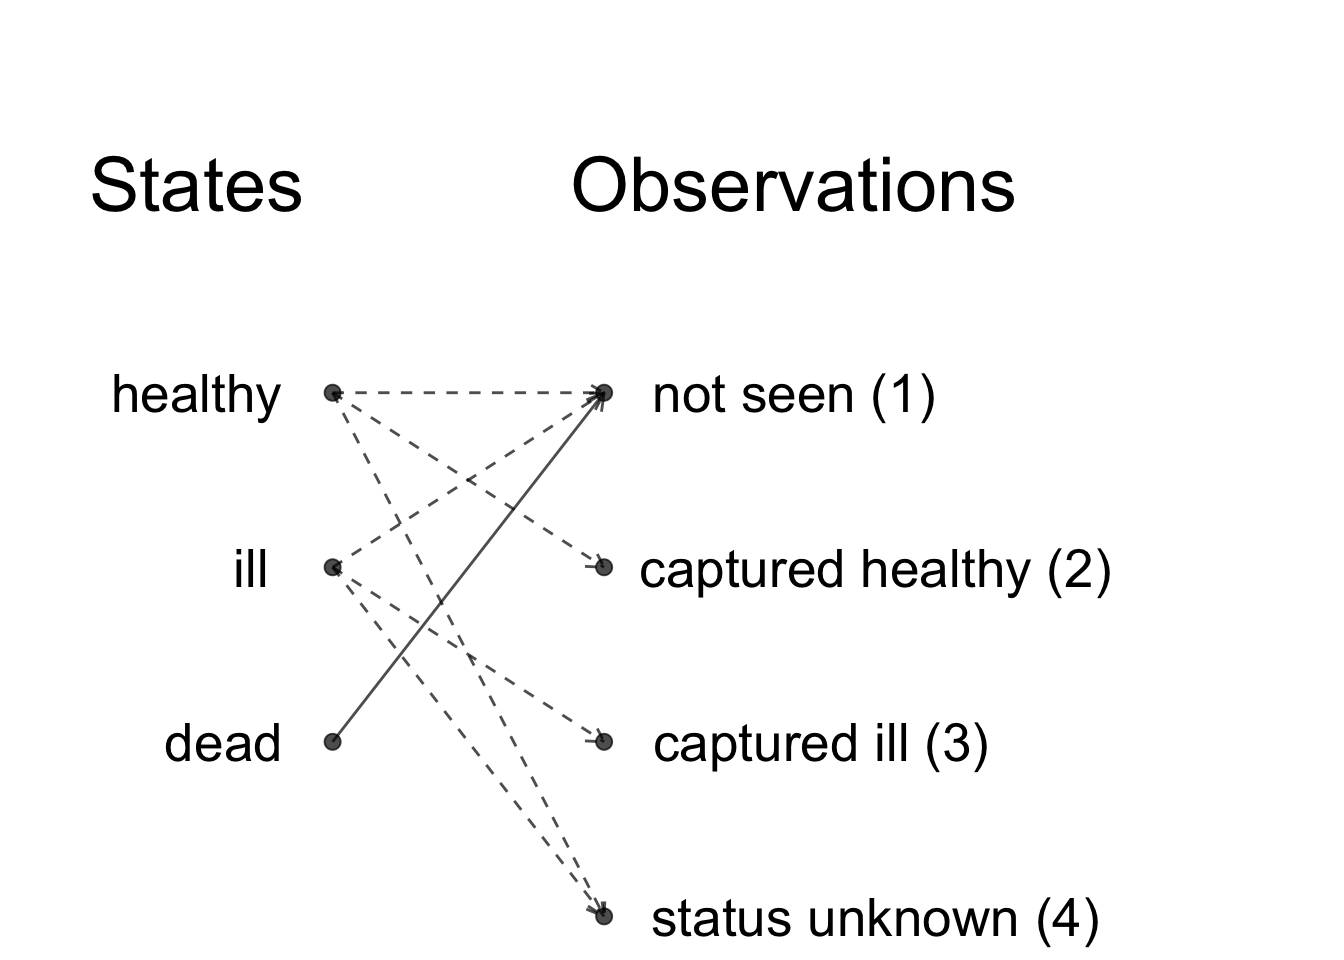
\includegraphics{banana-book_files/figure-latex/unnamed-chunk-60-1.pdf}
Time-dependent (covariate constrained) survival probability estimates. Caterpillar plot of the survival estimates. Survival between 1982 and 1983 seems to have been affected highly by a huge water flow compared to the other years. Coherent with previous section with flood effect.
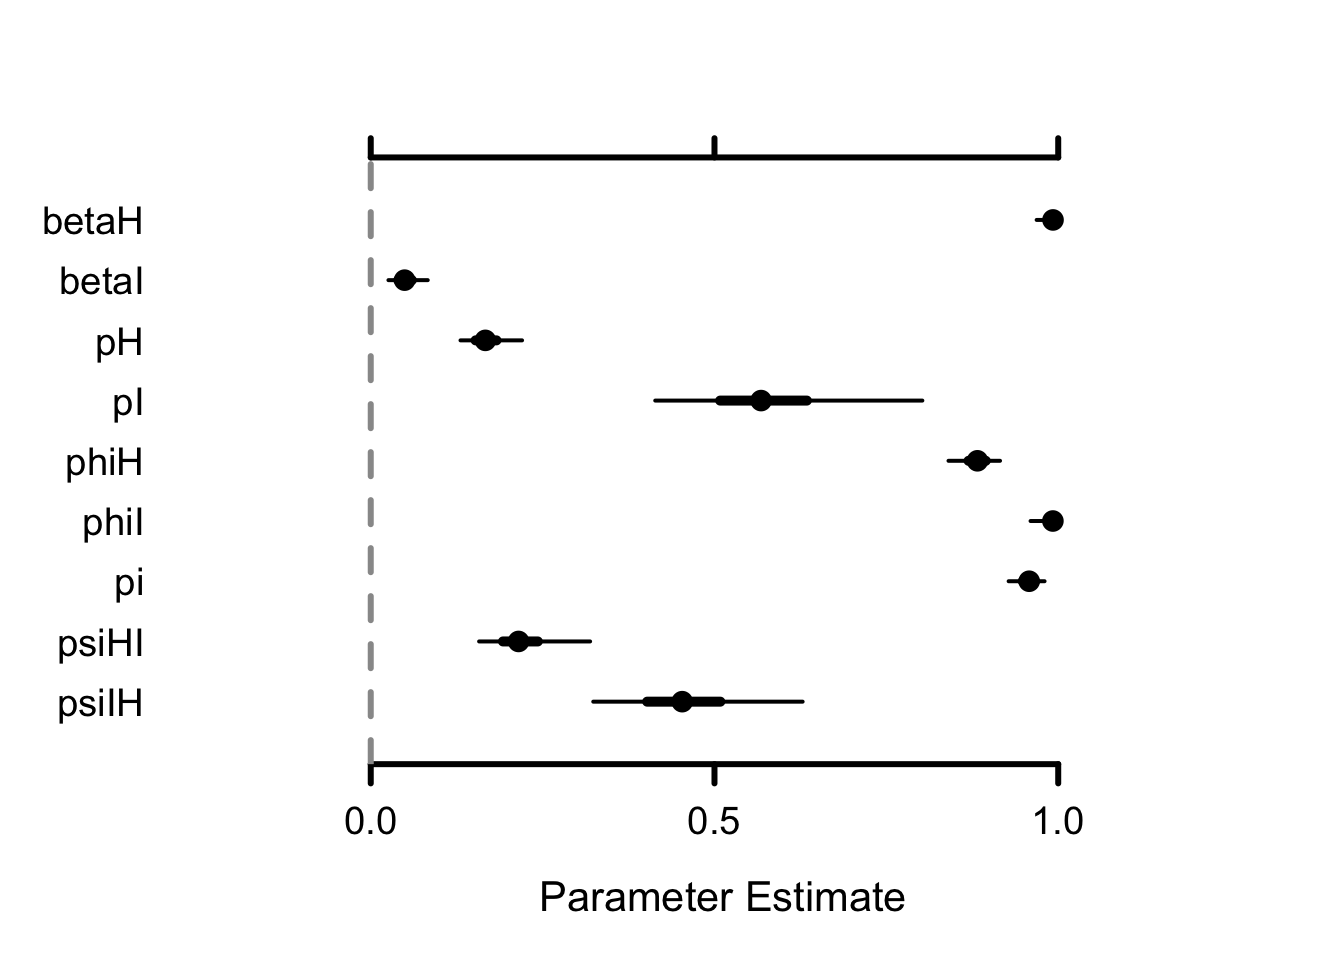
\includegraphics{banana-book_files/figure-latex/unnamed-chunk-61-1.pdf}

\hypertarget{individual-covariates}{%
\subsection{Individual covariates}\label{individual-covariates}}

\begin{itemize}
\item
  Discrete covariate like, e.g., sex
\item
  Continuous covariate like, e.g., mass or size
\end{itemize}

Sex and wing length in Dipper

\hypertarget{discrete-1}{%
\subsubsection{Discrete}\label{discrete-1}}

Sex effect

\begin{itemize}
\item
  Let's use a covariate \(\text{sex}\) that takes value 0 if male, and 1 if female
\item
  And write \(\text{logit}(\phi_i) = \beta_1 + \beta_2 \; \text{sex}_i\) for bird \(i\)
\item
  Then male survival is
\end{itemize}

\[\text{logit}(\phi_i) = \beta_1\]

\begin{itemize}
\tightlist
\item
  And female survival is
\end{itemize}

\[\text{logit}(\phi_i) = \beta_1 + \beta_2\]

Nimble implementation with sex as a covariate

\begin{Shaded}
\begin{Highlighting}[]
\NormalTok{hmm.phisexp }\OtherTok{\textless{}{-}} \FunctionTok{nimbleCode}\NormalTok{(\{}
\NormalTok{...}
  \ControlFlowTok{for}\NormalTok{ (i }\ControlFlowTok{in} \DecValTok{1}\SpecialCharTok{:}\NormalTok{N)\{ }\CommentTok{\#\textless{}\textless{}}
    \FunctionTok{logit}\NormalTok{(phi[i]) }\OtherTok{\textless{}{-}}\NormalTok{ beta[}\DecValTok{1}\NormalTok{] }\SpecialCharTok{+}\NormalTok{ beta[}\DecValTok{2}\NormalTok{] }\SpecialCharTok{*}\NormalTok{ sex[i]}
\NormalTok{    gamma[}\DecValTok{1}\NormalTok{,}\DecValTok{1}\NormalTok{,i] }\OtherTok{\textless{}{-}}\NormalTok{ phi[i]      }\CommentTok{\# Pr(alive t {-}\textgreater{} alive t+1)}
\NormalTok{    gamma[}\DecValTok{1}\NormalTok{,}\DecValTok{2}\NormalTok{,i] }\OtherTok{\textless{}{-}} \DecValTok{1} \SpecialCharTok{{-}}\NormalTok{ phi[i]  }\CommentTok{\# Pr(alive t {-}\textgreater{} dead t+1)}
\NormalTok{    gamma[}\DecValTok{2}\NormalTok{,}\DecValTok{1}\NormalTok{,i] }\OtherTok{\textless{}{-}} \DecValTok{0}        \CommentTok{\# Pr(dead t {-}\textgreater{} alive t+1)}
\NormalTok{    gamma[}\DecValTok{2}\NormalTok{,}\DecValTok{2}\NormalTok{,i] }\OtherTok{\textless{}{-}} \DecValTok{1}        \CommentTok{\# Pr(dead t {-}\textgreater{} dead t+1)}
\NormalTok{  \} }\CommentTok{\#\textless{}\textless{}}
\NormalTok{  beta[}\DecValTok{1}\NormalTok{] }\SpecialCharTok{\textasciitilde{}} \FunctionTok{dnorm}\NormalTok{(}\AttributeTok{mean =} \DecValTok{0}\NormalTok{, }\AttributeTok{sd =} \FloatTok{1.5}\NormalTok{)}
\NormalTok{  beta[}\DecValTok{2}\NormalTok{] }\SpecialCharTok{\textasciitilde{}} \FunctionTok{dnorm}\NormalTok{(}\AttributeTok{mean =} \DecValTok{0}\NormalTok{, }\AttributeTok{sd =} \FloatTok{1.5}\NormalTok{)}
\NormalTok{  phi\_male }\OtherTok{\textless{}{-}} \DecValTok{1}\SpecialCharTok{/}\NormalTok{(}\DecValTok{1}\SpecialCharTok{+}\FunctionTok{exp}\NormalTok{(}\SpecialCharTok{{-}}\NormalTok{beta[}\DecValTok{1}\NormalTok{]))}
\NormalTok{  phi\_female }\OtherTok{\textless{}{-}} \DecValTok{1}\SpecialCharTok{/}\NormalTok{(}\DecValTok{1}\SpecialCharTok{+}\FunctionTok{exp}\NormalTok{(}\SpecialCharTok{{-}}\NormalTok{(beta[}\DecValTok{1}\NormalTok{]}\SpecialCharTok{+}\NormalTok{beta[}\DecValTok{2}\NormalTok{])))}
\NormalTok{...}
  \CommentTok{\# likelihood}
  \ControlFlowTok{for}\NormalTok{ (i }\ControlFlowTok{in} \DecValTok{1}\SpecialCharTok{:}\NormalTok{N)\{}
\NormalTok{    z[i,first[i]] }\SpecialCharTok{\textasciitilde{}} \FunctionTok{dcat}\NormalTok{(delta[}\DecValTok{1}\SpecialCharTok{:}\DecValTok{2}\NormalTok{])}
    \ControlFlowTok{for}\NormalTok{ (j }\ControlFlowTok{in}\NormalTok{ (first[i]}\SpecialCharTok{+}\DecValTok{1}\NormalTok{)}\SpecialCharTok{:}\NormalTok{T)\{}
\NormalTok{      z[i,j] }\SpecialCharTok{\textasciitilde{}} \FunctionTok{dcat}\NormalTok{(gamma[z[i,j}\DecValTok{{-}1}\NormalTok{], }\DecValTok{1}\SpecialCharTok{:}\DecValTok{2}\NormalTok{, i])}
\NormalTok{      y[i,j] }\SpecialCharTok{\textasciitilde{}} \FunctionTok{dcat}\NormalTok{(omega[z[i,j], }\DecValTok{1}\SpecialCharTok{:}\DecValTok{2}\NormalTok{])}
\NormalTok{    \}}
\NormalTok{  \}}
\NormalTok{\})}
\end{Highlighting}
\end{Shaded}

\begin{verbatim}
##             mean   sd  2.5%   50% 97.5% Rhat n.eff
## beta[1]     0.29 0.14  0.01  0.29  0.57 1.01   237
## beta[2]    -0.09 0.19 -0.47 -0.10  0.29 1.01   241
## p           0.90 0.03  0.83  0.90  0.95 1.02   253
## phi_female  0.55 0.04  0.48  0.55  0.62 1.02   698
## phi_male    0.57 0.03  0.50  0.57  0.64 1.01   237
\end{verbatim}

NIMBLE implementation with nested indexing

\begin{itemize}
\tightlist
\item
  Let's use a covariate \(\text{sex}\) that contains 1s and 2s, indicating the sex of each individual: 1 if male, and 2 if female
\end{itemize}

\begin{Shaded}
\begin{Highlighting}[]
\NormalTok{...}
\ControlFlowTok{for}\NormalTok{ (i }\ControlFlowTok{in} \DecValTok{1}\SpecialCharTok{:}\NormalTok{N)\{}
\NormalTok{  phi[i] }\OtherTok{\textless{}{-}}\NormalTok{ beta[sex[i]]}
\NormalTok{  gamma[}\DecValTok{1}\NormalTok{,}\DecValTok{1}\NormalTok{,i] }\OtherTok{\textless{}{-}}\NormalTok{ phi[i]      }\CommentTok{\# Pr(alive t {-}\textgreater{} alive t+1)}
\NormalTok{  gamma[}\DecValTok{1}\NormalTok{,}\DecValTok{2}\NormalTok{,i] }\OtherTok{\textless{}{-}} \DecValTok{1} \SpecialCharTok{{-}}\NormalTok{ phi[i]  }\CommentTok{\# Pr(alive t {-}\textgreater{} dead t+1)}
\NormalTok{  gamma[}\DecValTok{2}\NormalTok{,}\DecValTok{1}\NormalTok{,i] }\OtherTok{\textless{}{-}} \DecValTok{0}           \CommentTok{\# Pr(dead t {-}\textgreater{} alive t+1)}
\NormalTok{  gamma[}\DecValTok{2}\NormalTok{,}\DecValTok{2}\NormalTok{,i] }\OtherTok{\textless{}{-}} \DecValTok{1}           \CommentTok{\# Pr(dead t {-}\textgreater{} dead t+1)}
\NormalTok{\}}
\NormalTok{beta[}\DecValTok{1}\NormalTok{] }\SpecialCharTok{\textasciitilde{}} \FunctionTok{dunif}\NormalTok{(}\DecValTok{0}\NormalTok{,}\DecValTok{1}\NormalTok{) }\CommentTok{\# male survival \#\textless{}\textless{}}
\NormalTok{beta[}\DecValTok{2}\NormalTok{] }\SpecialCharTok{\textasciitilde{}} \FunctionTok{dunif}\NormalTok{(}\DecValTok{0}\NormalTok{,}\DecValTok{1}\NormalTok{) }\CommentTok{\# female survival \#\textless{}\textless{}}
\NormalTok{...}
\end{Highlighting}
\end{Shaded}

\begin{itemize}
\tightlist
\item
  E.g. for individual \(i = 2\), \texttt{beta{[}sex{[}i{]}{]}} gives \texttt{beta{[}sex{[}2{]}{]}} which will be \texttt{beta{[}1{]}} or \texttt{beta{[}2{]}} depending on whether sex{[}2{]} is 1 or 2.
\end{itemize}

\begin{verbatim}
##         mean   sd 2.5%  50% 97.5% Rhat n.eff
## beta[1] 0.57 0.03 0.50 0.57  0.63 1.00   616
## beta[2] 0.55 0.03 0.48 0.55  0.62 1.02   657
## p       0.90 0.03 0.83 0.90  0.95 1.10   229
\end{verbatim}

\hypertarget{continuous-1}{%
\subsubsection{Continuous}\label{continuous-1}}

\begin{Shaded}
\begin{Highlighting}[]
\NormalTok{...}
  \ControlFlowTok{for}\NormalTok{ (i }\ControlFlowTok{in} \DecValTok{1}\SpecialCharTok{:}\NormalTok{N)\{ }\CommentTok{\#\textless{}\textless{}}
    \FunctionTok{logit}\NormalTok{(phi[i]) }\OtherTok{\textless{}{-}}\NormalTok{ beta[}\DecValTok{1}\NormalTok{] }\SpecialCharTok{+}\NormalTok{ beta[}\DecValTok{2}\NormalTok{] }\SpecialCharTok{*}\NormalTok{ winglength[i] }\CommentTok{\#\textless{}\textless{}}
\NormalTok{    gamma[}\DecValTok{1}\NormalTok{,}\DecValTok{1}\NormalTok{,i] }\OtherTok{\textless{}{-}}\NormalTok{ phi[i]      }\CommentTok{\# Pr(alive t {-}\textgreater{} alive t+1)}
\NormalTok{    gamma[}\DecValTok{1}\NormalTok{,}\DecValTok{2}\NormalTok{,i] }\OtherTok{\textless{}{-}} \DecValTok{1} \SpecialCharTok{{-}}\NormalTok{ phi[i]  }\CommentTok{\# Pr(alive t {-}\textgreater{} dead t+1)}
\NormalTok{    gamma[}\DecValTok{2}\NormalTok{,}\DecValTok{1}\NormalTok{,i] }\OtherTok{\textless{}{-}} \DecValTok{0}        \CommentTok{\# Pr(dead t {-}\textgreater{} alive t+1)}
\NormalTok{    gamma[}\DecValTok{2}\NormalTok{,}\DecValTok{2}\NormalTok{,i] }\OtherTok{\textless{}{-}} \DecValTok{1}        \CommentTok{\# Pr(dead t {-}\textgreater{} dead t+1)}
\NormalTok{  \}}
\NormalTok{  beta[}\DecValTok{1}\NormalTok{] }\SpecialCharTok{\textasciitilde{}} \FunctionTok{dnorm}\NormalTok{(}\AttributeTok{mean =} \DecValTok{0}\NormalTok{, }\AttributeTok{sd =} \FloatTok{1.5}\NormalTok{) }\CommentTok{\# intercept \#\textless{}\textless{}}
\NormalTok{  beta[}\DecValTok{2}\NormalTok{] }\SpecialCharTok{\textasciitilde{}} \FunctionTok{dnorm}\NormalTok{(}\AttributeTok{mean =} \DecValTok{0}\NormalTok{, }\AttributeTok{sd =} \FloatTok{1.5}\NormalTok{) }\CommentTok{\# slope \#\textless{}\textless{}}
\NormalTok{...}
\end{Highlighting}
\end{Shaded}

\begin{Shaded}
\begin{Highlighting}[]
\NormalTok{dipper }\OtherTok{\textless{}{-}} \FunctionTok{read\_csv}\NormalTok{(}\StringTok{"dat/dipper.csv"}\NormalTok{)}
\NormalTok{y }\OtherTok{\textless{}{-}}\NormalTok{ dipper }\SpecialCharTok{\%\textgreater{}\%}
  \FunctionTok{select}\NormalTok{(year\_1981}\SpecialCharTok{:}\NormalTok{year\_1987) }\SpecialCharTok{\%\textgreater{}\%}
  \FunctionTok{as.matrix}\NormalTok{()}
\end{Highlighting}
\end{Shaded}

Besides discrete individual covariates, you might want to have continuous individual covariates, e.g.~wing length in the dipper case study. Note that we're considering an individual trait that takes the same value whatever the occasion. If we were to have time-varying individual covariate in the model, we would have to do something about missing values of the covariate when an individual is not recaptured. The easiest way to cope with time-varying individual covariate is to discretize and treat levels of the covariates as states. More in the next live demo. Back to wing length. We first standardize the covariate.

\begin{Shaded}
\begin{Highlighting}[]
\NormalTok{wing.length.st }\OtherTok{\textless{}{-}} \FunctionTok{as.vector}\NormalTok{(}\FunctionTok{scale}\NormalTok{(dipper}\SpecialCharTok{$}\NormalTok{wing\_length))}
\FunctionTok{head}\NormalTok{(wing.length.st)}
\DocumentationTok{\#\# [1]  0.7581 {-}0.8671  0.5260 {-}1.5637 {-}1.3315  1.2225}
\end{Highlighting}
\end{Shaded}

Now we write the model. Basically we replace sex by wing length in the first method we used in the previous section. Easy.

\begin{Shaded}
\begin{Highlighting}[]
\NormalTok{hmm.phiwlp }\OtherTok{\textless{}{-}} \FunctionTok{nimbleCode}\NormalTok{(\{}
\NormalTok{    p }\SpecialCharTok{\textasciitilde{}} \FunctionTok{dunif}\NormalTok{(}\DecValTok{0}\NormalTok{, }\DecValTok{1}\NormalTok{) }\CommentTok{\# prior detection}
\NormalTok{    omega[}\DecValTok{1}\NormalTok{,}\DecValTok{1}\NormalTok{] }\OtherTok{\textless{}{-}} \DecValTok{1} \SpecialCharTok{{-}}\NormalTok{ p    }\CommentTok{\# Pr(alive t {-}\textgreater{} non{-}detected t)}
\NormalTok{    omega[}\DecValTok{1}\NormalTok{,}\DecValTok{2}\NormalTok{] }\OtherTok{\textless{}{-}}\NormalTok{ p        }\CommentTok{\# Pr(alive t {-}\textgreater{} detected t)}
\NormalTok{    omega[}\DecValTok{2}\NormalTok{,}\DecValTok{1}\NormalTok{] }\OtherTok{\textless{}{-}} \DecValTok{1}        \CommentTok{\# Pr(dead t {-}\textgreater{} non{-}detected t)}
\NormalTok{    omega[}\DecValTok{2}\NormalTok{,}\DecValTok{2}\NormalTok{] }\OtherTok{\textless{}{-}} \DecValTok{0}        \CommentTok{\# Pr(dead t {-}\textgreater{} detected t)}
  \ControlFlowTok{for}\NormalTok{ (i }\ControlFlowTok{in} \DecValTok{1}\SpecialCharTok{:}\NormalTok{N)\{}
    \FunctionTok{logit}\NormalTok{(phi[i]) }\OtherTok{\textless{}{-}}\NormalTok{ beta[}\DecValTok{1}\NormalTok{] }\SpecialCharTok{+}\NormalTok{ beta[}\DecValTok{2}\NormalTok{] }\SpecialCharTok{*}\NormalTok{ winglength[i]}
\NormalTok{    gamma[}\DecValTok{1}\NormalTok{,}\DecValTok{1}\NormalTok{,i] }\OtherTok{\textless{}{-}}\NormalTok{ phi[i]      }\CommentTok{\# Pr(alive t {-}\textgreater{} alive t+1)}
\NormalTok{    gamma[}\DecValTok{1}\NormalTok{,}\DecValTok{2}\NormalTok{,i] }\OtherTok{\textless{}{-}} \DecValTok{1} \SpecialCharTok{{-}}\NormalTok{ phi[i]  }\CommentTok{\# Pr(alive t {-}\textgreater{} dead t+1)}
\NormalTok{    gamma[}\DecValTok{2}\NormalTok{,}\DecValTok{1}\NormalTok{,i] }\OtherTok{\textless{}{-}} \DecValTok{0}           \CommentTok{\# Pr(dead t {-}\textgreater{} alive t+1)}
\NormalTok{    gamma[}\DecValTok{2}\NormalTok{,}\DecValTok{2}\NormalTok{,i] }\OtherTok{\textless{}{-}} \DecValTok{1}           \CommentTok{\# Pr(dead t {-}\textgreater{} dead t+1)}
\NormalTok{  \}}
\NormalTok{  beta[}\DecValTok{1}\NormalTok{] }\SpecialCharTok{\textasciitilde{}} \FunctionTok{dnorm}\NormalTok{(}\AttributeTok{mean =} \DecValTok{0}\NormalTok{, }\AttributeTok{sd =} \FloatTok{1.5}\NormalTok{)}
\NormalTok{  beta[}\DecValTok{2}\NormalTok{] }\SpecialCharTok{\textasciitilde{}} \FunctionTok{dnorm}\NormalTok{(}\AttributeTok{mean =} \DecValTok{0}\NormalTok{, }\AttributeTok{sd =} \FloatTok{1.5}\NormalTok{)}
\NormalTok{  delta[}\DecValTok{1}\NormalTok{] }\OtherTok{\textless{}{-}} \DecValTok{1}          \CommentTok{\# Pr(alive t = 1) = 1}
\NormalTok{  delta[}\DecValTok{2}\NormalTok{] }\OtherTok{\textless{}{-}} \DecValTok{0}          \CommentTok{\# Pr(dead t = 1) = 0}
  \CommentTok{\# likelihood}
  \ControlFlowTok{for}\NormalTok{ (i }\ControlFlowTok{in} \DecValTok{1}\SpecialCharTok{:}\NormalTok{N)\{}
\NormalTok{    z[i,first[i]] }\SpecialCharTok{\textasciitilde{}} \FunctionTok{dcat}\NormalTok{(delta[}\DecValTok{1}\SpecialCharTok{:}\DecValTok{2}\NormalTok{])}
    \ControlFlowTok{for}\NormalTok{ (j }\ControlFlowTok{in}\NormalTok{ (first[i]}\SpecialCharTok{+}\DecValTok{1}\NormalTok{)}\SpecialCharTok{:}\NormalTok{T)\{}
\NormalTok{      z[i,j] }\SpecialCharTok{\textasciitilde{}} \FunctionTok{dcat}\NormalTok{(gamma[z[i,j}\DecValTok{{-}1}\NormalTok{], }\DecValTok{1}\SpecialCharTok{:}\DecValTok{2}\NormalTok{, i])}
\NormalTok{      y[i,j] }\SpecialCharTok{\textasciitilde{}} \FunctionTok{dcat}\NormalTok{(omega[z[i,j], }\DecValTok{1}\SpecialCharTok{:}\DecValTok{2}\NormalTok{])}
\NormalTok{    \}}
\NormalTok{  \}}
\NormalTok{\})}
\end{Highlighting}
\end{Shaded}

Constants in a list.

\begin{Shaded}
\begin{Highlighting}[]
\NormalTok{my.constants }\OtherTok{\textless{}{-}} \FunctionTok{list}\NormalTok{(}\AttributeTok{N =} \FunctionTok{nrow}\NormalTok{(y), }
                     \AttributeTok{T =} \FunctionTok{ncol}\NormalTok{(y), }
                     \AttributeTok{first =}\NormalTok{ first,}
                     \AttributeTok{winglength =}\NormalTok{ wing.length.st)}
\end{Highlighting}
\end{Shaded}

Initial values.

\begin{Shaded}
\begin{Highlighting}[]
\NormalTok{initial.values }\OtherTok{\textless{}{-}} \ControlFlowTok{function}\NormalTok{() }\FunctionTok{list}\NormalTok{(}\AttributeTok{beta =} \FunctionTok{rnorm}\NormalTok{(}\DecValTok{2}\NormalTok{,}\DecValTok{0}\NormalTok{,}\DecValTok{1}\NormalTok{),}
                                  \AttributeTok{p =} \FunctionTok{runif}\NormalTok{(}\DecValTok{1}\NormalTok{,}\DecValTok{0}\NormalTok{,}\DecValTok{1}\NormalTok{),}
                                  \AttributeTok{z =}\NormalTok{ zinits)}
\end{Highlighting}
\end{Shaded}

Run nimble.

\begin{Shaded}
\begin{Highlighting}[]
\NormalTok{mcmc.phiwlp }\OtherTok{\textless{}{-}} \FunctionTok{nimbleMCMC}\NormalTok{(}\AttributeTok{code =}\NormalTok{ hmm.phiwlp, }
                          \AttributeTok{constants =}\NormalTok{ my.constants,}
                          \AttributeTok{data =}\NormalTok{ my.data,              }
                          \AttributeTok{inits =}\NormalTok{ initial.values,}
                          \AttributeTok{monitors =}\NormalTok{ parameters.to.save,}
                          \AttributeTok{niter =}\NormalTok{ n.iter,}
                          \AttributeTok{nburnin =}\NormalTok{ n.burnin, }
                          \AttributeTok{nchains =}\NormalTok{ n.chains)}
\DocumentationTok{\#\# |{-}{-}{-}{-}{-}{-}{-}{-}{-}{-}{-}{-}{-}|{-}{-}{-}{-}{-}{-}{-}{-}{-}{-}{-}{-}{-}|{-}{-}{-}{-}{-}{-}{-}{-}{-}{-}{-}{-}{-}|{-}{-}{-}{-}{-}{-}{-}{-}{-}{-}{-}{-}{-}|}
\DocumentationTok{\#\# |{-}{-}{-}{-}{-}{-}{-}{-}{-}{-}{-}{-}{-}{-}{-}{-}{-}{-}{-}{-}{-}{-}{-}{-}{-}{-}{-}{-}{-}{-}{-}{-}{-}{-}{-}{-}{-}{-}{-}{-}{-}{-}{-}{-}{-}{-}{-}{-}{-}{-}{-}{-}{-}{-}{-}|}
\DocumentationTok{\#\# |{-}{-}{-}{-}{-}{-}{-}{-}{-}{-}{-}{-}{-}|{-}{-}{-}{-}{-}{-}{-}{-}{-}{-}{-}{-}{-}|{-}{-}{-}{-}{-}{-}{-}{-}{-}{-}{-}{-}{-}|{-}{-}{-}{-}{-}{-}{-}{-}{-}{-}{-}{-}{-}|}
\DocumentationTok{\#\# |{-}{-}{-}{-}{-}{-}{-}{-}{-}{-}{-}{-}{-}{-}{-}{-}{-}{-}{-}{-}{-}{-}{-}{-}{-}{-}{-}{-}{-}{-}{-}{-}{-}{-}{-}{-}{-}{-}{-}{-}{-}{-}{-}{-}{-}{-}{-}{-}{-}{-}{-}{-}{-}{-}{-}|}
\end{Highlighting}
\end{Shaded}

Numerical summaries. Wing length does not seem to explain much individual-to-individual variation in survival. See corresponding slope param.

\begin{Shaded}
\begin{Highlighting}[]
\FunctionTok{load}\NormalTok{(here}\SpecialCharTok{::}\FunctionTok{here}\NormalTok{(}\StringTok{"dat/phiwlp.RData"}\NormalTok{))}
\FunctionTok{MCMCsummary}\NormalTok{(mcmc.phiwlp, }\AttributeTok{params =} \StringTok{"beta"}\NormalTok{, }\AttributeTok{round =} \DecValTok{2}\NormalTok{)}
\DocumentationTok{\#\#          mean   sd  2.5\%   50\% 97.5\% Rhat n.eff}
\DocumentationTok{\#\# beta[1]  0.25 0.10  0.04  0.25  0.45    1  1472}
\DocumentationTok{\#\# beta[2] {-}0.02 0.09 {-}0.20 {-}0.02  0.17    1  1555}
\end{Highlighting}
\end{Shaded}

Let's plot the relationship. First, we gather the values generated from the posterior distribution of the regression parameters in the two chains.

\begin{Shaded}
\begin{Highlighting}[]
\NormalTok{beta1 }\OtherTok{\textless{}{-}} \FunctionTok{c}\NormalTok{(mcmc.phiwlp}\SpecialCharTok{$}\NormalTok{chain1[,}\StringTok{\textquotesingle{}beta[1]\textquotesingle{}}\NormalTok{], mcmc.phiwlp}\SpecialCharTok{$}\NormalTok{chain2[,}\StringTok{\textquotesingle{}beta[1]\textquotesingle{}}\NormalTok{])}
\NormalTok{beta2 }\OtherTok{\textless{}{-}} \FunctionTok{c}\NormalTok{(mcmc.phiwlp}\SpecialCharTok{$}\NormalTok{chain1[,}\StringTok{\textquotesingle{}beta[2]\textquotesingle{}}\NormalTok{], mcmc.phiwlp}\SpecialCharTok{$}\NormalTok{chain2[,}\StringTok{\textquotesingle{}beta[2]\textquotesingle{}}\NormalTok{])}
\end{Highlighting}
\end{Shaded}

Then we define a grid of values for wing length, and predict survival for each MCMC iteration.

\begin{Shaded}
\begin{Highlighting}[]
\NormalTok{predicted\_survival }\OtherTok{\textless{}{-}} \FunctionTok{matrix}\NormalTok{(}\ConstantTok{NA}\NormalTok{, }\AttributeTok{nrow =} \FunctionTok{length}\NormalTok{(beta1), }\AttributeTok{ncol =} \FunctionTok{length}\NormalTok{(my.constants}\SpecialCharTok{$}\NormalTok{winglength))}
\ControlFlowTok{for}\NormalTok{ (i }\ControlFlowTok{in} \DecValTok{1}\SpecialCharTok{:}\FunctionTok{length}\NormalTok{(beta1))\{}
  \ControlFlowTok{for}\NormalTok{ (j }\ControlFlowTok{in} \DecValTok{1}\SpecialCharTok{:}\FunctionTok{length}\NormalTok{(my.constants}\SpecialCharTok{$}\NormalTok{winglength))\{}
\NormalTok{    predicted\_survival[i,j] }\OtherTok{\textless{}{-}} \FunctionTok{plogis}\NormalTok{(beta1[i] }\SpecialCharTok{+}\NormalTok{ beta2[i] }\SpecialCharTok{*}\NormalTok{ my.constants}\SpecialCharTok{$}\NormalTok{winglength[j])}
\NormalTok{  \}}
\NormalTok{\}}
\end{Highlighting}
\end{Shaded}

Now we calculate posterior mean and the credible interval. Note the ordering.

\begin{Shaded}
\begin{Highlighting}[]
\NormalTok{mean\_survival }\OtherTok{\textless{}{-}} \FunctionTok{apply}\NormalTok{(predicted\_survival, }\DecValTok{2}\NormalTok{, mean)}
\NormalTok{lci }\OtherTok{\textless{}{-}} \FunctionTok{apply}\NormalTok{(predicted\_survival, }\DecValTok{2}\NormalTok{, quantile, }\AttributeTok{prob =} \FloatTok{2.5}\SpecialCharTok{/}\DecValTok{100}\NormalTok{)}
\NormalTok{uci }\OtherTok{\textless{}{-}} \FunctionTok{apply}\NormalTok{(predicted\_survival, }\DecValTok{2}\NormalTok{, quantile, }\AttributeTok{prob =} \FloatTok{97.5}\SpecialCharTok{/}\DecValTok{100}\NormalTok{)}
\NormalTok{ord }\OtherTok{\textless{}{-}} \FunctionTok{order}\NormalTok{(my.constants}\SpecialCharTok{$}\NormalTok{winglength)}
\NormalTok{df }\OtherTok{\textless{}{-}} \FunctionTok{data.frame}\NormalTok{(}\AttributeTok{wing\_length =}\NormalTok{ my.constants}\SpecialCharTok{$}\NormalTok{winglength[ord],}
                 \AttributeTok{survival =}\NormalTok{ mean\_survival[ord],}
                 \AttributeTok{lci =}\NormalTok{ lci[ord],}
                 \AttributeTok{uci =}\NormalTok{ uci[ord])}
\end{Highlighting}
\end{Shaded}

Now time to visualize.

\begin{Shaded}
\begin{Highlighting}[]
\NormalTok{df }\SpecialCharTok{\%\textgreater{}\%}
  \FunctionTok{ggplot}\NormalTok{() }\SpecialCharTok{+} 
  \FunctionTok{aes}\NormalTok{(}\AttributeTok{x =}\NormalTok{ wing\_length, }\AttributeTok{y =}\NormalTok{ survival) }\SpecialCharTok{+} 
  \FunctionTok{geom\_line}\NormalTok{() }\SpecialCharTok{+} 
  \FunctionTok{geom\_ribbon}\NormalTok{(}\FunctionTok{aes}\NormalTok{(}\AttributeTok{ymin =}\NormalTok{ lci, }\AttributeTok{ymax =}\NormalTok{ uci), }\AttributeTok{fill =} \StringTok{"grey70"}\NormalTok{, }\AttributeTok{alpha =} \FloatTok{0.5}\NormalTok{) }\SpecialCharTok{+} 
  \FunctionTok{ylim}\NormalTok{(}\DecValTok{0}\NormalTok{,}\DecValTok{1}\NormalTok{) }\SpecialCharTok{+} 
  \FunctionTok{labs}\NormalTok{(}\AttributeTok{x =} \StringTok{"wing length"}\NormalTok{, }\AttributeTok{y =} \StringTok{"estimated survival"}\NormalTok{)}
\end{Highlighting}
\end{Shaded}

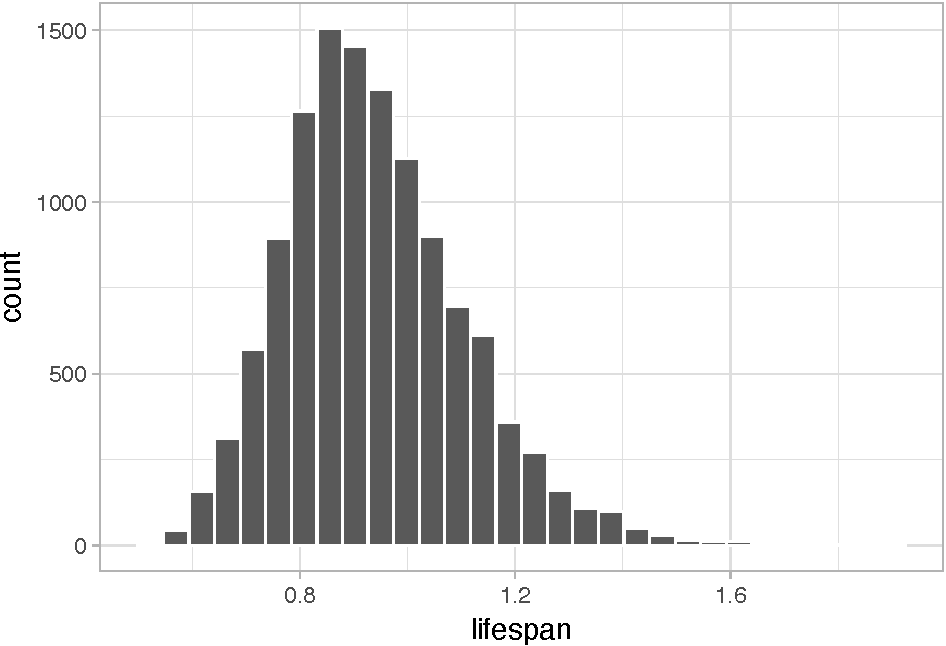
\includegraphics{banana-book_files/figure-latex/unnamed-chunk-78-1.pdf}
Wing length

\hypertarget{additive-and-interaction}{%
\subsection{Additive and interaction}\label{additive-and-interaction}}

You may test an effect of both sex and wing length. Write the model. We use nested indexing with the sex index that contains 1 if the bird is a male, and 2 otherwise. We have \(\logit(\phi_i) = \beta_1 + \beta_3 * \text{winglength}_i\) for males, and \(\logit(\phi_i) = \beta_2 + \beta_3 * \text{winglength}_i\) for females.

\begin{Shaded}
\begin{Highlighting}[]
\NormalTok{hmm.phisexwlp }\OtherTok{\textless{}{-}} \FunctionTok{nimbleCode}\NormalTok{(\{}
\NormalTok{  p }\SpecialCharTok{\textasciitilde{}} \FunctionTok{dunif}\NormalTok{(}\DecValTok{0}\NormalTok{, }\DecValTok{1}\NormalTok{) }\CommentTok{\# prior detection}
\NormalTok{  omega[}\DecValTok{1}\NormalTok{,}\DecValTok{1}\NormalTok{] }\OtherTok{\textless{}{-}} \DecValTok{1} \SpecialCharTok{{-}}\NormalTok{ p    }\CommentTok{\# Pr(alive t {-}\textgreater{} non{-}detected t)}
\NormalTok{  omega[}\DecValTok{1}\NormalTok{,}\DecValTok{2}\NormalTok{] }\OtherTok{\textless{}{-}}\NormalTok{ p        }\CommentTok{\# Pr(alive t {-}\textgreater{} detected t)}
\NormalTok{  omega[}\DecValTok{2}\NormalTok{,}\DecValTok{1}\NormalTok{] }\OtherTok{\textless{}{-}} \DecValTok{1}        \CommentTok{\# Pr(dead t {-}\textgreater{} non{-}detected t)}
\NormalTok{  omega[}\DecValTok{2}\NormalTok{,}\DecValTok{2}\NormalTok{] }\OtherTok{\textless{}{-}} \DecValTok{0}        \CommentTok{\# Pr(dead t {-}\textgreater{} detected t)}
  \ControlFlowTok{for}\NormalTok{ (i }\ControlFlowTok{in} \DecValTok{1}\SpecialCharTok{:}\NormalTok{N)\{}
    \FunctionTok{logit}\NormalTok{(phi[i]) }\OtherTok{\textless{}{-}}\NormalTok{ beta[sex[i]] }\SpecialCharTok{+}\NormalTok{ beta[}\DecValTok{3}\NormalTok{] }\SpecialCharTok{*}\NormalTok{ winglength[i]}
\NormalTok{    gamma[}\DecValTok{1}\NormalTok{,}\DecValTok{1}\NormalTok{,i] }\OtherTok{\textless{}{-}}\NormalTok{ phi[i]      }\CommentTok{\# Pr(alive t {-}\textgreater{} alive t+1)}
\NormalTok{    gamma[}\DecValTok{1}\NormalTok{,}\DecValTok{2}\NormalTok{,i] }\OtherTok{\textless{}{-}} \DecValTok{1} \SpecialCharTok{{-}}\NormalTok{ phi[i]  }\CommentTok{\# Pr(alive t {-}\textgreater{} dead t+1)}
\NormalTok{    gamma[}\DecValTok{2}\NormalTok{,}\DecValTok{1}\NormalTok{,i] }\OtherTok{\textless{}{-}} \DecValTok{0}           \CommentTok{\# Pr(dead t {-}\textgreater{} alive t+1)}
\NormalTok{    gamma[}\DecValTok{2}\NormalTok{,}\DecValTok{2}\NormalTok{,i] }\OtherTok{\textless{}{-}} \DecValTok{1}           \CommentTok{\# Pr(dead t {-}\textgreater{} dead t+1)}
\NormalTok{  \}}
\NormalTok{  beta[}\DecValTok{1}\NormalTok{] }\SpecialCharTok{\textasciitilde{}} \FunctionTok{dnorm}\NormalTok{(}\AttributeTok{mean =} \DecValTok{0}\NormalTok{, }\AttributeTok{sd =} \FloatTok{1.5}\NormalTok{) }\CommentTok{\# intercept male}
\NormalTok{  beta[}\DecValTok{2}\NormalTok{] }\SpecialCharTok{\textasciitilde{}} \FunctionTok{dnorm}\NormalTok{(}\AttributeTok{mean =} \DecValTok{0}\NormalTok{, }\AttributeTok{sd =} \FloatTok{1.5}\NormalTok{) }\CommentTok{\# intercept female}
\NormalTok{  beta[}\DecValTok{3}\NormalTok{] }\SpecialCharTok{\textasciitilde{}} \FunctionTok{dnorm}\NormalTok{(}\AttributeTok{mean =} \DecValTok{0}\NormalTok{, }\AttributeTok{sd =} \FloatTok{1.5}\NormalTok{) }\CommentTok{\# slope wing length}
\NormalTok{  delta[}\DecValTok{1}\NormalTok{] }\OtherTok{\textless{}{-}} \DecValTok{1}          \CommentTok{\# Pr(alive t = 1) = 1}
\NormalTok{  delta[}\DecValTok{2}\NormalTok{] }\OtherTok{\textless{}{-}} \DecValTok{0}          \CommentTok{\# Pr(dead t = 1) = 0}
  \CommentTok{\# likelihood}
  \ControlFlowTok{for}\NormalTok{ (i }\ControlFlowTok{in} \DecValTok{1}\SpecialCharTok{:}\NormalTok{N)\{}
\NormalTok{    z[i,first[i]] }\SpecialCharTok{\textasciitilde{}} \FunctionTok{dcat}\NormalTok{(delta[}\DecValTok{1}\SpecialCharTok{:}\DecValTok{2}\NormalTok{])}
    \ControlFlowTok{for}\NormalTok{ (j }\ControlFlowTok{in}\NormalTok{ (first[i]}\SpecialCharTok{+}\DecValTok{1}\NormalTok{)}\SpecialCharTok{:}\NormalTok{T)\{}
\NormalTok{      z[i,j] }\SpecialCharTok{\textasciitilde{}} \FunctionTok{dcat}\NormalTok{(gamma[z[i,j}\DecValTok{{-}1}\NormalTok{], }\DecValTok{1}\SpecialCharTok{:}\DecValTok{2}\NormalTok{, i])}
\NormalTok{      y[i,j] }\SpecialCharTok{\textasciitilde{}} \FunctionTok{dcat}\NormalTok{(omega[z[i,j], }\DecValTok{1}\SpecialCharTok{:}\DecValTok{2}\NormalTok{])}
\NormalTok{    \}}
\NormalTok{  \}}
\NormalTok{\})}
\end{Highlighting}
\end{Shaded}

Constants in a list. Note we standardise wing length.

\begin{Shaded}
\begin{Highlighting}[]
\NormalTok{first }\OtherTok{\textless{}{-}} \FunctionTok{apply}\NormalTok{(y, }\DecValTok{1}\NormalTok{, }\ControlFlowTok{function}\NormalTok{(x) }\FunctionTok{min}\NormalTok{(}\FunctionTok{which}\NormalTok{(x }\SpecialCharTok{!=}\DecValTok{0}\NormalTok{)))}
\NormalTok{wing.length.st }\OtherTok{\textless{}{-}} \FunctionTok{as.vector}\NormalTok{(}\FunctionTok{scale}\NormalTok{(dipper}\SpecialCharTok{$}\NormalTok{wing\_length))}
\NormalTok{my.constants }\OtherTok{\textless{}{-}} \FunctionTok{list}\NormalTok{(}\AttributeTok{N =} \FunctionTok{nrow}\NormalTok{(y), }
                     \AttributeTok{T =} \FunctionTok{ncol}\NormalTok{(y), }
                     \AttributeTok{first =}\NormalTok{ first,}
                     \AttributeTok{winglength =}\NormalTok{ wing.length.st,}
                     \AttributeTok{sex =} \FunctionTok{if\_else}\NormalTok{(dipper}\SpecialCharTok{$}\NormalTok{sex }\SpecialCharTok{==} \StringTok{"M"}\NormalTok{, }\DecValTok{1}\NormalTok{, }\DecValTok{2}\NormalTok{))}
\NormalTok{my.data }\OtherTok{\textless{}{-}} \FunctionTok{list}\NormalTok{(}\AttributeTok{y =}\NormalTok{ y }\SpecialCharTok{+} \DecValTok{1}\NormalTok{)}
\end{Highlighting}
\end{Shaded}

Data in a list.

\begin{Shaded}
\begin{Highlighting}[]
\NormalTok{my.data }\OtherTok{\textless{}{-}} \FunctionTok{list}\NormalTok{(}\AttributeTok{y =}\NormalTok{ y }\SpecialCharTok{+} \DecValTok{1}\NormalTok{)}
\end{Highlighting}
\end{Shaded}

Initial values.

\begin{Shaded}
\begin{Highlighting}[]
\NormalTok{zinits }\OtherTok{\textless{}{-}}\NormalTok{ y}
\NormalTok{zinits[zinits }\SpecialCharTok{==} \DecValTok{0}\NormalTok{] }\OtherTok{\textless{}{-}} \DecValTok{1}
\NormalTok{initial.values }\OtherTok{\textless{}{-}} \ControlFlowTok{function}\NormalTok{() }\FunctionTok{list}\NormalTok{(}\AttributeTok{beta =} \FunctionTok{rnorm}\NormalTok{(}\DecValTok{3}\NormalTok{,}\DecValTok{0}\NormalTok{,}\DecValTok{5}\NormalTok{),}
                                  \AttributeTok{p =} \FunctionTok{runif}\NormalTok{(}\DecValTok{1}\NormalTok{,}\DecValTok{0}\NormalTok{,}\DecValTok{1}\NormalTok{),}
                                  \AttributeTok{z =}\NormalTok{ zinits)}
\end{Highlighting}
\end{Shaded}

Parameters to be monitored.

\begin{Shaded}
\begin{Highlighting}[]
\NormalTok{parameters.to.save }\OtherTok{\textless{}{-}} \FunctionTok{c}\NormalTok{(}\StringTok{"beta"}\NormalTok{, }\StringTok{"p"}\NormalTok{)}
\end{Highlighting}
\end{Shaded}

MCMC details.

\begin{Shaded}
\begin{Highlighting}[]
\NormalTok{n.iter }\OtherTok{\textless{}{-}} \DecValTok{5000}
\NormalTok{n.burnin }\OtherTok{\textless{}{-}} \DecValTok{2500}
\NormalTok{n.chains }\OtherTok{\textless{}{-}} \DecValTok{2}
\end{Highlighting}
\end{Shaded}

Run nimble.

\begin{Shaded}
\begin{Highlighting}[]
\NormalTok{mcmc.phisexwlp }\OtherTok{\textless{}{-}} \FunctionTok{nimbleMCMC}\NormalTok{(}\AttributeTok{code =}\NormalTok{ hmm.phisexwlp, }
                             \AttributeTok{constants =}\NormalTok{ my.constants,}
                             \AttributeTok{data =}\NormalTok{ my.data,              }
                             \AttributeTok{inits =}\NormalTok{ initial.values,}
                             \AttributeTok{monitors =}\NormalTok{ parameters.to.save,}
                             \AttributeTok{niter =}\NormalTok{ n.iter,}
                             \AttributeTok{nburnin =}\NormalTok{ n.burnin, }
                             \AttributeTok{nchains =}\NormalTok{ n.chains)}
\end{Highlighting}
\end{Shaded}

Display results.

\begin{verbatim}
##          mean   sd  2.5%   50% 97.5% Rhat n.eff
## beta[1]  0.52 0.23  0.07  0.53  0.96 1.01   223
## beta[2] -0.02 0.22 -0.47 -0.02  0.42 1.02   199
## beta[3] -0.25 0.19 -0.61 -0.25  0.14 1.02   144
## p        0.90 0.03  0.83  0.90  0.95 1.02   466
\end{verbatim}

Let's visualise survival as a function of wing length for both sexes.

First we put together the values from the two chains we generated in the posterior distributions of the regression parameters.

\begin{Shaded}
\begin{Highlighting}[]
\NormalTok{beta1 }\OtherTok{\textless{}{-}} \FunctionTok{c}\NormalTok{(mcmc.phisexwlp}\SpecialCharTok{$}\NormalTok{chain1[,}\StringTok{\textquotesingle{}beta[1]\textquotesingle{}}\NormalTok{], mcmc.phisexwlp}\SpecialCharTok{$}\NormalTok{chain2[,}\StringTok{\textquotesingle{}beta[1]\textquotesingle{}}\NormalTok{])}
\NormalTok{beta2 }\OtherTok{\textless{}{-}} \FunctionTok{c}\NormalTok{(mcmc.phisexwlp}\SpecialCharTok{$}\NormalTok{chain1[,}\StringTok{\textquotesingle{}beta[2]\textquotesingle{}}\NormalTok{], mcmc.phisexwlp}\SpecialCharTok{$}\NormalTok{chain2[,}\StringTok{\textquotesingle{}beta[2]\textquotesingle{}}\NormalTok{])}
\NormalTok{beta3 }\OtherTok{\textless{}{-}} \FunctionTok{c}\NormalTok{(mcmc.phisexwlp}\SpecialCharTok{$}\NormalTok{chain1[,}\StringTok{\textquotesingle{}beta[3]\textquotesingle{}}\NormalTok{], mcmc.phisexwlp}\SpecialCharTok{$}\NormalTok{chain2[,}\StringTok{\textquotesingle{}beta[3]\textquotesingle{}}\NormalTok{])}
\end{Highlighting}
\end{Shaded}

We get survival estimates for each MCMC iteration.

\begin{Shaded}
\begin{Highlighting}[]
\NormalTok{predicted\_survivalM }\OtherTok{\textless{}{-}} \FunctionTok{matrix}\NormalTok{(}\ConstantTok{NA}\NormalTok{, }\AttributeTok{nrow =} \FunctionTok{length}\NormalTok{(beta1), }\AttributeTok{ncol =} \FunctionTok{length}\NormalTok{(my.constants}\SpecialCharTok{$}\NormalTok{winglength))}
\NormalTok{predicted\_survivalF }\OtherTok{\textless{}{-}} \FunctionTok{matrix}\NormalTok{(}\ConstantTok{NA}\NormalTok{, }\AttributeTok{nrow =} \FunctionTok{length}\NormalTok{(beta1), }\AttributeTok{ncol =} \FunctionTok{length}\NormalTok{(my.constants}\SpecialCharTok{$}\NormalTok{winglength))}
\ControlFlowTok{for}\NormalTok{ (i }\ControlFlowTok{in} \DecValTok{1}\SpecialCharTok{:}\FunctionTok{length}\NormalTok{(beta1))\{}
  \ControlFlowTok{for}\NormalTok{ (j }\ControlFlowTok{in} \DecValTok{1}\SpecialCharTok{:}\FunctionTok{length}\NormalTok{(my.constants}\SpecialCharTok{$}\NormalTok{winglength))\{}
\NormalTok{    predicted\_survivalM[i,j] }\OtherTok{\textless{}{-}} \FunctionTok{plogis}\NormalTok{(beta1[i] }\SpecialCharTok{+}\NormalTok{ beta3[i] }\SpecialCharTok{*}\NormalTok{ my.constants}\SpecialCharTok{$}\NormalTok{winglength[j]) }\CommentTok{\# males}
\NormalTok{    predicted\_survivalF[i,j] }\OtherTok{\textless{}{-}} \FunctionTok{plogis}\NormalTok{(beta2[i] }\SpecialCharTok{+}\NormalTok{ beta3[i] }\SpecialCharTok{*}\NormalTok{ my.constants}\SpecialCharTok{$}\NormalTok{winglength[j]) }\CommentTok{\# females}
\NormalTok{  \}}
\NormalTok{\}}
\end{Highlighting}
\end{Shaded}

From here, we may calculate posterior mean and credible intervals.

\begin{Shaded}
\begin{Highlighting}[]
\NormalTok{mean\_survivalM }\OtherTok{\textless{}{-}} \FunctionTok{apply}\NormalTok{(predicted\_survivalM, }\DecValTok{2}\NormalTok{, mean)}
\NormalTok{lciM }\OtherTok{\textless{}{-}} \FunctionTok{apply}\NormalTok{(predicted\_survivalM, }\DecValTok{2}\NormalTok{, quantile, }\AttributeTok{prob =} \FloatTok{2.5}\SpecialCharTok{/}\DecValTok{100}\NormalTok{)}
\NormalTok{uciM }\OtherTok{\textless{}{-}} \FunctionTok{apply}\NormalTok{(predicted\_survivalM, }\DecValTok{2}\NormalTok{, quantile, }\AttributeTok{prob =} \FloatTok{97.5}\SpecialCharTok{/}\DecValTok{100}\NormalTok{)}
\NormalTok{mean\_survivalF }\OtherTok{\textless{}{-}} \FunctionTok{apply}\NormalTok{(predicted\_survivalF, }\DecValTok{2}\NormalTok{, mean)}
\NormalTok{lciF }\OtherTok{\textless{}{-}} \FunctionTok{apply}\NormalTok{(predicted\_survivalF, }\DecValTok{2}\NormalTok{, quantile, }\AttributeTok{prob =} \FloatTok{2.5}\SpecialCharTok{/}\DecValTok{100}\NormalTok{)}
\NormalTok{uciF }\OtherTok{\textless{}{-}} \FunctionTok{apply}\NormalTok{(predicted\_survivalF, }\DecValTok{2}\NormalTok{, quantile, }\AttributeTok{prob =} \FloatTok{97.5}\SpecialCharTok{/}\DecValTok{100}\NormalTok{)}
\NormalTok{ord }\OtherTok{\textless{}{-}} \FunctionTok{order}\NormalTok{(my.constants}\SpecialCharTok{$}\NormalTok{winglength)}
\NormalTok{df }\OtherTok{\textless{}{-}} \FunctionTok{data.frame}\NormalTok{(}\AttributeTok{wing\_length =} \FunctionTok{c}\NormalTok{(my.constants}\SpecialCharTok{$}\NormalTok{winglength[ord], my.constants}\SpecialCharTok{$}\NormalTok{winglength[ord]),}
                 \AttributeTok{survival =} \FunctionTok{c}\NormalTok{(mean\_survivalM[ord], mean\_survivalF[ord]),}
                 \AttributeTok{lci =} \FunctionTok{c}\NormalTok{(lciM[ord],lciF[ord]),}
                 \AttributeTok{uci =} \FunctionTok{c}\NormalTok{(uciM[ord],uciF[ord]),}
                 \AttributeTok{sex =} \FunctionTok{c}\NormalTok{(}\FunctionTok{rep}\NormalTok{(}\StringTok{"male"}\NormalTok{, }\FunctionTok{length}\NormalTok{(mean\_survivalM)), }\FunctionTok{rep}\NormalTok{(}\StringTok{"female"}\NormalTok{, }\FunctionTok{length}\NormalTok{(mean\_survivalF))))}
\end{Highlighting}
\end{Shaded}

Now on a plot.

\begin{Shaded}
\begin{Highlighting}[]
\NormalTok{df }\SpecialCharTok{\%\textgreater{}\%}
  \FunctionTok{ggplot}\NormalTok{() }\SpecialCharTok{+} 
  \FunctionTok{aes}\NormalTok{(}\AttributeTok{x =}\NormalTok{ wing\_length, }\AttributeTok{y =}\NormalTok{ survival, }\AttributeTok{color =}\NormalTok{ sex) }\SpecialCharTok{+} 
  \FunctionTok{geom\_line}\NormalTok{() }\SpecialCharTok{+} 
  \FunctionTok{geom\_ribbon}\NormalTok{(}\FunctionTok{aes}\NormalTok{(}\AttributeTok{ymin =}\NormalTok{ lci, }\AttributeTok{ymax =}\NormalTok{ uci, }\AttributeTok{fill =}\NormalTok{ sex), }\AttributeTok{alpha =} \FloatTok{0.5}\NormalTok{) }\SpecialCharTok{+} 
  \FunctionTok{ylim}\NormalTok{(}\DecValTok{0}\NormalTok{,}\DecValTok{1}\NormalTok{) }\SpecialCharTok{+} 
  \FunctionTok{labs}\NormalTok{(}\AttributeTok{x =} \StringTok{"wing length"}\NormalTok{, }\AttributeTok{y =} \StringTok{"estimated survival"}\NormalTok{, }\AttributeTok{color =} \StringTok{""}\NormalTok{, }\AttributeTok{fill =} \StringTok{""}\NormalTok{)}
\end{Highlighting}
\end{Shaded}

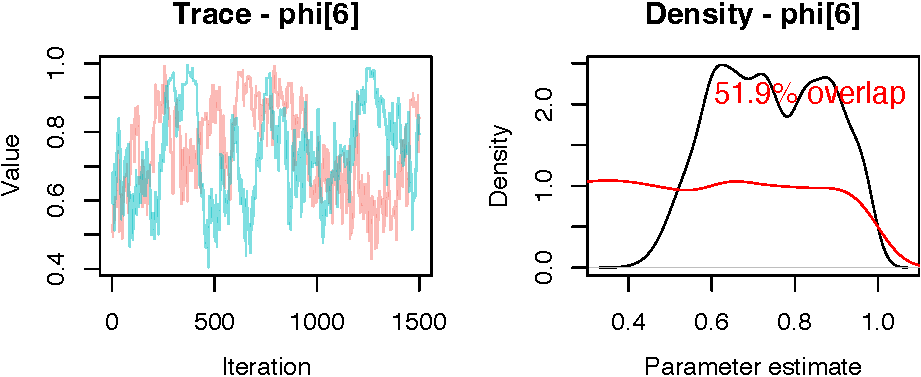
\includegraphics{banana-book_files/figure-latex/unnamed-chunk-91-1.pdf}

\hypertarget{random-effects}{%
\subsection{Random effects}\label{random-effects}}

\hypertarget{temporal}{%
\subsubsection{Temporal}\label{temporal}}

Include temporal covariates, say \(x_t\) with \(\text{logit}(\phi_t) = \beta_1 + \beta_2 x_t\). If temporal variation not fully explained by covariates, add random effects \(\text{logit}(\phi_t) = \beta_1 + \beta_2 x_t + \varepsilon_t, \; \varepsilon_t \sim N(0,\sigma^2)\). We may wish to allow for extra variation in the survival vs.~water flow relationship. To do so, we consider a yearly random effect. The prior on the standard deviation of the random effect is uniform between 0 and 10.

\begin{Shaded}
\begin{Highlighting}[]
\NormalTok{hmm.phiflowREpt }\OtherTok{\textless{}{-}} \FunctionTok{nimbleCode}\NormalTok{(\{}
\NormalTok{  delta[}\DecValTok{1}\NormalTok{] }\OtherTok{\textless{}{-}} \DecValTok{1}          \CommentTok{\# Pr(alive t = 1) = 1}
\NormalTok{  delta[}\DecValTok{2}\NormalTok{] }\OtherTok{\textless{}{-}} \DecValTok{0}          \CommentTok{\# Pr(dead t = 1) = 0}
  \ControlFlowTok{for}\NormalTok{ (t }\ControlFlowTok{in} \DecValTok{1}\SpecialCharTok{:}\NormalTok{(T}\DecValTok{{-}1}\NormalTok{))\{}
    \FunctionTok{logit}\NormalTok{(phi[t]) }\OtherTok{\textless{}{-}}\NormalTok{ beta[}\DecValTok{1}\NormalTok{] }\SpecialCharTok{+}\NormalTok{ beta[}\DecValTok{2}\NormalTok{] }\SpecialCharTok{*}\NormalTok{ flow[t] }\SpecialCharTok{+}\NormalTok{ eps[t] }\CommentTok{\# eps is random effect}
\NormalTok{    eps[t] }\SpecialCharTok{\textasciitilde{}} \FunctionTok{dnorm}\NormalTok{(}\DecValTok{0}\NormalTok{, }\AttributeTok{sd =}\NormalTok{ sdeps) }
\NormalTok{    gamma[}\DecValTok{1}\NormalTok{,}\DecValTok{1}\NormalTok{,t] }\OtherTok{\textless{}{-}}\NormalTok{ phi[t]      }\CommentTok{\# Pr(alive t {-}\textgreater{} alive t+1)}
\NormalTok{    gamma[}\DecValTok{1}\NormalTok{,}\DecValTok{2}\NormalTok{,t] }\OtherTok{\textless{}{-}} \DecValTok{1} \SpecialCharTok{{-}}\NormalTok{ phi[t]  }\CommentTok{\# Pr(alive t {-}\textgreater{} dead t+1)}
\NormalTok{    gamma[}\DecValTok{2}\NormalTok{,}\DecValTok{1}\NormalTok{,t] }\OtherTok{\textless{}{-}} \DecValTok{0}           \CommentTok{\# Pr(dead t {-}\textgreater{} alive t+1)}
\NormalTok{    gamma[}\DecValTok{2}\NormalTok{,}\DecValTok{2}\NormalTok{,t] }\OtherTok{\textless{}{-}} \DecValTok{1}           \CommentTok{\# Pr(dead t {-}\textgreater{} dead t+1)}
\NormalTok{    p[t] }\SpecialCharTok{\textasciitilde{}} \FunctionTok{dunif}\NormalTok{(}\DecValTok{0}\NormalTok{, }\DecValTok{1}\NormalTok{)          }\CommentTok{\# prior detection}
\NormalTok{    omega[}\DecValTok{1}\NormalTok{,}\DecValTok{1}\NormalTok{,t] }\OtherTok{\textless{}{-}} \DecValTok{1} \SpecialCharTok{{-}}\NormalTok{ p[t]    }\CommentTok{\# Pr(alive t {-}\textgreater{} non{-}detected t)}
\NormalTok{    omega[}\DecValTok{1}\NormalTok{,}\DecValTok{2}\NormalTok{,t] }\OtherTok{\textless{}{-}}\NormalTok{ p[t]        }\CommentTok{\# Pr(alive t {-}\textgreater{} detected t)}
\NormalTok{    omega[}\DecValTok{2}\NormalTok{,}\DecValTok{1}\NormalTok{,t] }\OtherTok{\textless{}{-}} \DecValTok{1}           \CommentTok{\# Pr(dead t {-}\textgreater{} non{-}detected t)}
\NormalTok{    omega[}\DecValTok{2}\NormalTok{,}\DecValTok{2}\NormalTok{,t] }\OtherTok{\textless{}{-}} \DecValTok{0}           \CommentTok{\# Pr(dead t {-}\textgreater{} detected t)}
\NormalTok{  \}}
\NormalTok{  beta[}\DecValTok{1}\NormalTok{] }\SpecialCharTok{\textasciitilde{}} \FunctionTok{dnorm}\NormalTok{(}\DecValTok{0}\NormalTok{, }\FloatTok{1.5}\NormalTok{) }\CommentTok{\# prior intercept}
\NormalTok{  beta[}\DecValTok{2}\NormalTok{] }\SpecialCharTok{\textasciitilde{}} \FunctionTok{dnorm}\NormalTok{(}\DecValTok{0}\NormalTok{, }\FloatTok{1.5}\NormalTok{) }\CommentTok{\# prior slope}
\NormalTok{  sdeps }\SpecialCharTok{\textasciitilde{}} \FunctionTok{dunif}\NormalTok{(}\DecValTok{0}\NormalTok{,}\DecValTok{10}\NormalTok{)}
  \CommentTok{\# likelihood}
  \ControlFlowTok{for}\NormalTok{ (i }\ControlFlowTok{in} \DecValTok{1}\SpecialCharTok{:}\NormalTok{N)\{}
\NormalTok{    z[i,first[i]] }\SpecialCharTok{\textasciitilde{}} \FunctionTok{dcat}\NormalTok{(delta[}\DecValTok{1}\SpecialCharTok{:}\DecValTok{2}\NormalTok{])}
    \ControlFlowTok{for}\NormalTok{ (j }\ControlFlowTok{in}\NormalTok{ (first[i]}\SpecialCharTok{+}\DecValTok{1}\NormalTok{)}\SpecialCharTok{:}\NormalTok{T)\{}
\NormalTok{      z[i,j] }\SpecialCharTok{\textasciitilde{}} \FunctionTok{dcat}\NormalTok{(gamma[z[i,j}\DecValTok{{-}1}\NormalTok{], }\DecValTok{1}\SpecialCharTok{:}\DecValTok{2}\NormalTok{, j}\DecValTok{{-}1}\NormalTok{])}
\NormalTok{      y[i,j] }\SpecialCharTok{\textasciitilde{}} \FunctionTok{dcat}\NormalTok{(omega[z[i,j], }\DecValTok{1}\SpecialCharTok{:}\DecValTok{2}\NormalTok{, j}\DecValTok{{-}1}\NormalTok{])}
\NormalTok{    \}}
\NormalTok{  \}}
\NormalTok{\})}
\end{Highlighting}
\end{Shaded}

Initial values.

\begin{Shaded}
\begin{Highlighting}[]
\NormalTok{initial.values }\OtherTok{\textless{}{-}} \ControlFlowTok{function}\NormalTok{() }\FunctionTok{list}\NormalTok{(}\AttributeTok{beta =} \FunctionTok{rnorm}\NormalTok{(}\DecValTok{2}\NormalTok{,}\DecValTok{0}\NormalTok{,}\DecValTok{1}\NormalTok{),}
                                  \AttributeTok{p =} \FunctionTok{runif}\NormalTok{(my.constants}\SpecialCharTok{$}\NormalTok{T}\DecValTok{{-}1}\NormalTok{,}\DecValTok{0}\NormalTok{,}\DecValTok{1}\NormalTok{),}
                                  \AttributeTok{sdeps =} \FunctionTok{runif}\NormalTok{(}\DecValTok{1}\NormalTok{,}\DecValTok{0}\NormalTok{,}\DecValTok{3}\NormalTok{),}
                                  \AttributeTok{z =}\NormalTok{ zinits)}
\end{Highlighting}
\end{Shaded}

Parameters to be monitored.

\begin{Shaded}
\begin{Highlighting}[]
\NormalTok{parameters.to.save }\OtherTok{\textless{}{-}} \FunctionTok{c}\NormalTok{(}\StringTok{"beta"}\NormalTok{, }\StringTok{"p"}\NormalTok{, }\StringTok{"phi"}\NormalTok{, }\StringTok{"sdeps"}\NormalTok{)}
\end{Highlighting}
\end{Shaded}

MCMC details. Note that we've increased the number of iterations and the length of the burn-in period.

\begin{Shaded}
\begin{Highlighting}[]
\NormalTok{n.iter }\OtherTok{\textless{}{-}} \DecValTok{10000}
\NormalTok{n.burnin }\OtherTok{\textless{}{-}} \DecValTok{5000}
\NormalTok{n.chains }\OtherTok{\textless{}{-}} \DecValTok{2}
\end{Highlighting}
\end{Shaded}

Run nimble.

\begin{Shaded}
\begin{Highlighting}[]
\NormalTok{mcmc.phiflowREpt }\OtherTok{\textless{}{-}} \FunctionTok{nimbleMCMC}\NormalTok{(}\AttributeTok{code =}\NormalTok{ hmm.phiflowREpt, }
                             \AttributeTok{constants =}\NormalTok{ my.constants,}
                             \AttributeTok{data =}\NormalTok{ my.data,              }
                             \AttributeTok{inits =}\NormalTok{ initial.values,}
                             \AttributeTok{monitors =}\NormalTok{ parameters.to.save,}
                             \AttributeTok{niter =}\NormalTok{ n.iter,}
                             \AttributeTok{nburnin =}\NormalTok{ n.burnin, }
                             \AttributeTok{nchains =}\NormalTok{ n.chains)}
\end{Highlighting}
\end{Shaded}

Display outputs. Seems that the water flow effect is not so important anymore.

\begin{Shaded}
\begin{Highlighting}[]
\FunctionTok{load}\NormalTok{(here}\SpecialCharTok{::}\FunctionTok{here}\NormalTok{(}\StringTok{"dat/phiflowREpt.RData"}\NormalTok{))}
\FunctionTok{MCMCsummary}\NormalTok{(}\AttributeTok{object =}\NormalTok{ mcmc.phiflowREpt, }\AttributeTok{round =} \DecValTok{2}\NormalTok{)}
\DocumentationTok{\#\#          mean   sd  2.5\%   50\% 97.5\% Rhat n.eff}
\DocumentationTok{\#\# beta[1]  0.27 0.25 {-}0.32  0.28  0.77 1.04   153}
\DocumentationTok{\#\# beta[2] {-}0.22 0.23 {-}0.65 {-}0.23  0.31 1.01   300}
\DocumentationTok{\#\# p[1]     0.70 0.13  0.44  0.71  0.92 1.00  1414}
\DocumentationTok{\#\# p[2]     0.88 0.07  0.70  0.89  0.98 1.00   971}
\DocumentationTok{\#\# p[3]     0.87 0.07  0.71  0.88  0.97 1.00   981}
\DocumentationTok{\#\# p[4]     0.88 0.05  0.75  0.88  0.96 1.01  1236}
\DocumentationTok{\#\# p[5]     0.91 0.05  0.80  0.91  0.98 1.00   974}
\DocumentationTok{\#\# p[6]     0.81 0.11  0.56  0.83  0.98 1.00   164}
\DocumentationTok{\#\# phi[1]   0.65 0.09  0.48  0.63  0.84 1.00   490}
\DocumentationTok{\#\# phi[2]   0.45 0.07  0.32  0.45  0.59 1.00  1853}
\DocumentationTok{\#\# phi[3]   0.53 0.06  0.41  0.53  0.63 1.00   660}
\DocumentationTok{\#\# phi[4]   0.62 0.05  0.52  0.62  0.73 1.00  1238}
\DocumentationTok{\#\# phi[5]   0.59 0.05  0.50  0.59  0.69 1.01  1061}
\DocumentationTok{\#\# phi[6]   0.64 0.10  0.50  0.62  0.91 1.00   143}
\DocumentationTok{\#\# sdeps    0.47 0.54  0.05  0.34  1.59 1.08    91}
\end{Highlighting}
\end{Shaded}

Trace plots for the standard deviation of the random effect.

\begin{Shaded}
\begin{Highlighting}[]
\FunctionTok{MCMCtrace}\NormalTok{(}\AttributeTok{object =}\NormalTok{ mcmc.phiflowREpt, }\AttributeTok{params =} \StringTok{"sdeps"}\NormalTok{, }\AttributeTok{pdf =} \ConstantTok{FALSE}\NormalTok{)}
\end{Highlighting}
\end{Shaded}

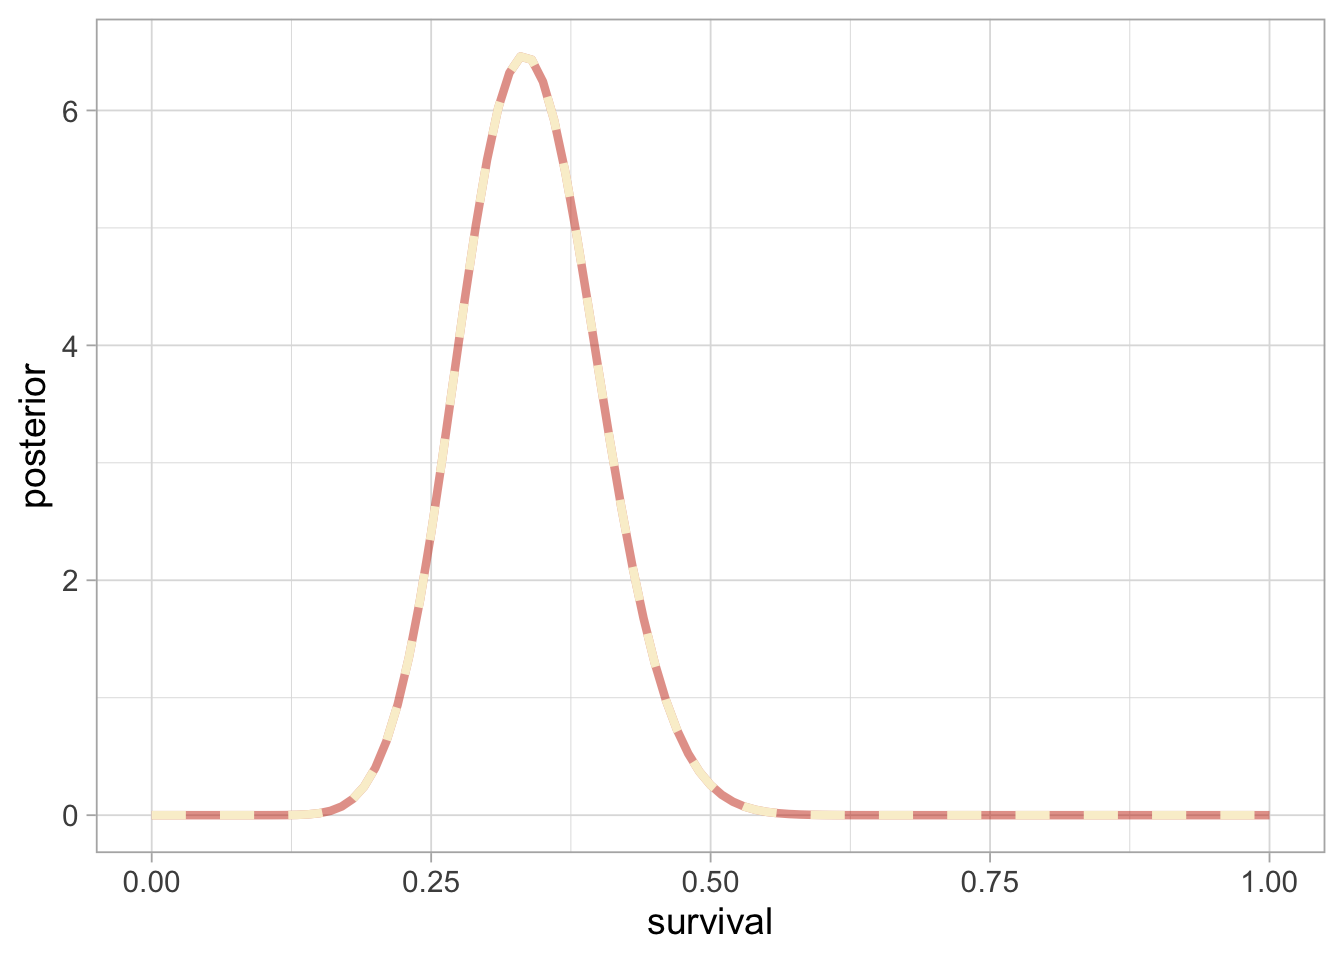
\includegraphics{banana-book_files/figure-latex/unnamed-chunk-98-1.pdf}

\hypertarget{individual}{%
\subsubsection{Individual}\label{individual}}

We add an individual random effect.

\begin{Shaded}
\begin{Highlighting}[]
\NormalTok{hmm.phiwlrep }\OtherTok{\textless{}{-}} \FunctionTok{nimbleCode}\NormalTok{(\{}
\NormalTok{    p }\SpecialCharTok{\textasciitilde{}} \FunctionTok{dunif}\NormalTok{(}\DecValTok{0}\NormalTok{, }\DecValTok{1}\NormalTok{) }\CommentTok{\# prior detection}
\NormalTok{    omega[}\DecValTok{1}\NormalTok{,}\DecValTok{1}\NormalTok{] }\OtherTok{\textless{}{-}} \DecValTok{1} \SpecialCharTok{{-}}\NormalTok{ p    }\CommentTok{\# Pr(alive t {-}\textgreater{} non{-}detected t)}
\NormalTok{    omega[}\DecValTok{1}\NormalTok{,}\DecValTok{2}\NormalTok{] }\OtherTok{\textless{}{-}}\NormalTok{ p        }\CommentTok{\# Pr(alive t {-}\textgreater{} detected t)}
\NormalTok{    omega[}\DecValTok{2}\NormalTok{,}\DecValTok{1}\NormalTok{] }\OtherTok{\textless{}{-}} \DecValTok{1}        \CommentTok{\# Pr(dead t {-}\textgreater{} non{-}detected t)}
\NormalTok{    omega[}\DecValTok{2}\NormalTok{,}\DecValTok{2}\NormalTok{] }\OtherTok{\textless{}{-}} \DecValTok{0}        \CommentTok{\# Pr(dead t {-}\textgreater{} detected t)}
  \ControlFlowTok{for}\NormalTok{ (i }\ControlFlowTok{in} \DecValTok{1}\SpecialCharTok{:}\NormalTok{N)\{}
    \FunctionTok{logit}\NormalTok{(phi[i]) }\OtherTok{\textless{}{-}}\NormalTok{ beta[}\DecValTok{1}\NormalTok{] }\SpecialCharTok{+}\NormalTok{ beta[}\DecValTok{2}\NormalTok{] }\SpecialCharTok{*}\NormalTok{ winglength[i] }\SpecialCharTok{+}\NormalTok{ eps[i]}
\NormalTok{    eps[i] }\SpecialCharTok{\textasciitilde{}} \FunctionTok{dnorm}\NormalTok{(}\AttributeTok{mean =} \DecValTok{0}\NormalTok{, }\AttributeTok{sd =}\NormalTok{ sdeps)}
\NormalTok{    gamma[}\DecValTok{1}\NormalTok{,}\DecValTok{1}\NormalTok{,i] }\OtherTok{\textless{}{-}}\NormalTok{ phi[i]      }\CommentTok{\# Pr(alive t {-}\textgreater{} alive t+1)}
\NormalTok{    gamma[}\DecValTok{1}\NormalTok{,}\DecValTok{2}\NormalTok{,i] }\OtherTok{\textless{}{-}} \DecValTok{1} \SpecialCharTok{{-}}\NormalTok{ phi[i]  }\CommentTok{\# Pr(alive t {-}\textgreater{} dead t+1)}
\NormalTok{    gamma[}\DecValTok{2}\NormalTok{,}\DecValTok{1}\NormalTok{,i] }\OtherTok{\textless{}{-}} \DecValTok{0}           \CommentTok{\# Pr(dead t {-}\textgreater{} alive t+1)}
\NormalTok{    gamma[}\DecValTok{2}\NormalTok{,}\DecValTok{2}\NormalTok{,i] }\OtherTok{\textless{}{-}} \DecValTok{1}           \CommentTok{\# Pr(dead t {-}\textgreater{} dead t+1)}
\NormalTok{  \}}
\NormalTok{  beta[}\DecValTok{1}\NormalTok{] }\SpecialCharTok{\textasciitilde{}} \FunctionTok{dnorm}\NormalTok{(}\AttributeTok{mean =} \DecValTok{0}\NormalTok{, }\AttributeTok{sd =} \FloatTok{1.5}\NormalTok{)}
\NormalTok{  beta[}\DecValTok{2}\NormalTok{] }\SpecialCharTok{\textasciitilde{}} \FunctionTok{dnorm}\NormalTok{(}\AttributeTok{mean =} \DecValTok{0}\NormalTok{, }\AttributeTok{sd =} \FloatTok{1.5}\NormalTok{)}
\NormalTok{  sdeps }\SpecialCharTok{\textasciitilde{}} \FunctionTok{dunif}\NormalTok{(}\DecValTok{0}\NormalTok{, }\DecValTok{10}\NormalTok{)}
\NormalTok{  delta[}\DecValTok{1}\NormalTok{] }\OtherTok{\textless{}{-}} \DecValTok{1}          \CommentTok{\# Pr(alive t = 1) = 1}
\NormalTok{  delta[}\DecValTok{2}\NormalTok{] }\OtherTok{\textless{}{-}} \DecValTok{0}          \CommentTok{\# Pr(dead t = 1) = 0}
  \CommentTok{\# likelihood}
  \ControlFlowTok{for}\NormalTok{ (i }\ControlFlowTok{in} \DecValTok{1}\SpecialCharTok{:}\NormalTok{N)\{}
\NormalTok{    z[i,first[i]] }\SpecialCharTok{\textasciitilde{}} \FunctionTok{dcat}\NormalTok{(delta[}\DecValTok{1}\SpecialCharTok{:}\DecValTok{2}\NormalTok{])}
    \ControlFlowTok{for}\NormalTok{ (j }\ControlFlowTok{in}\NormalTok{ (first[i]}\SpecialCharTok{+}\DecValTok{1}\NormalTok{)}\SpecialCharTok{:}\NormalTok{T)\{}
\NormalTok{      z[i,j] }\SpecialCharTok{\textasciitilde{}} \FunctionTok{dcat}\NormalTok{(gamma[z[i,j}\DecValTok{{-}1}\NormalTok{], }\DecValTok{1}\SpecialCharTok{:}\DecValTok{2}\NormalTok{, i])}
\NormalTok{      y[i,j] }\SpecialCharTok{\textasciitilde{}} \FunctionTok{dcat}\NormalTok{(omega[z[i,j], }\DecValTok{1}\SpecialCharTok{:}\DecValTok{2}\NormalTok{])}
\NormalTok{    \}}
\NormalTok{  \}}
\NormalTok{\})}
\end{Highlighting}
\end{Shaded}

Initial values.

\begin{Shaded}
\begin{Highlighting}[]
\NormalTok{initial.values }\OtherTok{\textless{}{-}} \ControlFlowTok{function}\NormalTok{() }\FunctionTok{list}\NormalTok{(}\AttributeTok{beta =} \FunctionTok{rnorm}\NormalTok{(}\DecValTok{2}\NormalTok{,}\DecValTok{0}\NormalTok{,}\FloatTok{1.5}\NormalTok{),}
                                  \AttributeTok{sdeps =} \FunctionTok{runif}\NormalTok{(}\DecValTok{1}\NormalTok{,}\DecValTok{0}\NormalTok{,}\DecValTok{3}\NormalTok{),}
                                  \AttributeTok{p =} \FunctionTok{runif}\NormalTok{(}\DecValTok{1}\NormalTok{,}\DecValTok{0}\NormalTok{,}\DecValTok{1}\NormalTok{),}
                                  \AttributeTok{z =}\NormalTok{ zinits)}
\end{Highlighting}
\end{Shaded}

Parameters to be monitored.

\begin{Shaded}
\begin{Highlighting}[]
\NormalTok{parameters.to.save }\OtherTok{\textless{}{-}} \FunctionTok{c}\NormalTok{(}\StringTok{"beta"}\NormalTok{, }\StringTok{"sdeps"}\NormalTok{, }\StringTok{"p"}\NormalTok{)}
\end{Highlighting}
\end{Shaded}

MCMC details. Note that we increase the number of iterations and the length of the burn-in period.

\begin{Shaded}
\begin{Highlighting}[]
\NormalTok{n.iter }\OtherTok{\textless{}{-}} \DecValTok{10000}
\NormalTok{n.burnin }\OtherTok{\textless{}{-}} \DecValTok{5000}
\NormalTok{n.chains }\OtherTok{\textless{}{-}} \DecValTok{2}
\end{Highlighting}
\end{Shaded}

Run nimble.

\begin{Shaded}
\begin{Highlighting}[]
\NormalTok{mcmc.phiwlrep }\OtherTok{\textless{}{-}} \FunctionTok{nimbleMCMC}\NormalTok{(}\AttributeTok{code =}\NormalTok{ hmm.phiwlrep, }
                            \AttributeTok{constants =}\NormalTok{ my.constants,}
                            \AttributeTok{data =}\NormalTok{ my.data,              }
                            \AttributeTok{inits =}\NormalTok{ initial.values,}
                            \AttributeTok{monitors =}\NormalTok{ parameters.to.save,}
                            \AttributeTok{niter =}\NormalTok{ n.iter,}
                            \AttributeTok{nburnin =}\NormalTok{ n.burnin, }
                            \AttributeTok{nchains =}\NormalTok{ n.chains)}
\end{Highlighting}
\end{Shaded}

Numerical summaries.

\begin{verbatim}
##          mean   sd  2.5%   50% 97.5% Rhat n.eff
## beta[1]  0.21 0.12 -0.04  0.21  0.43 1.00  1202
## beta[2] -0.01 0.10 -0.20 -0.01  0.19 1.00  1789
## p        0.90 0.03  0.83  0.90  0.95 1.01   790
## sdeps    0.40 0.26  0.02  0.37  0.95 1.01   170
\end{verbatim}

Effective sample size for SD very low. Let's try something else. We reparameterize by non-centering.

\begin{Shaded}
\begin{Highlighting}[]
\NormalTok{hmm.phiwlrep }\OtherTok{\textless{}{-}} \FunctionTok{nimbleCode}\NormalTok{(\{}
\NormalTok{    p }\SpecialCharTok{\textasciitilde{}} \FunctionTok{dunif}\NormalTok{(}\DecValTok{0}\NormalTok{, }\DecValTok{1}\NormalTok{) }\CommentTok{\# prior detection}
\NormalTok{    omega[}\DecValTok{1}\NormalTok{,}\DecValTok{1}\NormalTok{] }\OtherTok{\textless{}{-}} \DecValTok{1} \SpecialCharTok{{-}}\NormalTok{ p    }\CommentTok{\# Pr(alive t {-}\textgreater{} non{-}detected t)}
\NormalTok{    omega[}\DecValTok{1}\NormalTok{,}\DecValTok{2}\NormalTok{] }\OtherTok{\textless{}{-}}\NormalTok{ p        }\CommentTok{\# Pr(alive t {-}\textgreater{} detected t)}
\NormalTok{    omega[}\DecValTok{2}\NormalTok{,}\DecValTok{1}\NormalTok{] }\OtherTok{\textless{}{-}} \DecValTok{1}        \CommentTok{\# Pr(dead t {-}\textgreater{} non{-}detected t)}
\NormalTok{    omega[}\DecValTok{2}\NormalTok{,}\DecValTok{2}\NormalTok{] }\OtherTok{\textless{}{-}} \DecValTok{0}        \CommentTok{\# Pr(dead t {-}\textgreater{} detected t)}
  \ControlFlowTok{for}\NormalTok{ (i }\ControlFlowTok{in} \DecValTok{1}\SpecialCharTok{:}\NormalTok{N)\{}
    \FunctionTok{logit}\NormalTok{(phi[i]) }\OtherTok{\textless{}{-}}\NormalTok{ beta[}\DecValTok{1}\NormalTok{] }\SpecialCharTok{+}\NormalTok{ beta[}\DecValTok{2}\NormalTok{] }\SpecialCharTok{*}\NormalTok{ winglength[i] }\SpecialCharTok{+}\NormalTok{ sdeps }\SpecialCharTok{*}\NormalTok{ eps[i]}
\NormalTok{    eps[i] }\SpecialCharTok{\textasciitilde{}} \FunctionTok{dnorm}\NormalTok{(}\AttributeTok{mean =} \DecValTok{0}\NormalTok{, }\AttributeTok{sd =} \DecValTok{1}\NormalTok{)}
\NormalTok{    gamma[}\DecValTok{1}\NormalTok{,}\DecValTok{1}\NormalTok{,i] }\OtherTok{\textless{}{-}}\NormalTok{ phi[i]      }\CommentTok{\# Pr(alive t {-}\textgreater{} alive t+1)}
\NormalTok{    gamma[}\DecValTok{1}\NormalTok{,}\DecValTok{2}\NormalTok{,i] }\OtherTok{\textless{}{-}} \DecValTok{1} \SpecialCharTok{{-}}\NormalTok{ phi[i]  }\CommentTok{\# Pr(alive t {-}\textgreater{} dead t+1)}
\NormalTok{    gamma[}\DecValTok{2}\NormalTok{,}\DecValTok{1}\NormalTok{,i] }\OtherTok{\textless{}{-}} \DecValTok{0}           \CommentTok{\# Pr(dead t {-}\textgreater{} alive t+1)}
\NormalTok{    gamma[}\DecValTok{2}\NormalTok{,}\DecValTok{2}\NormalTok{,i] }\OtherTok{\textless{}{-}} \DecValTok{1}           \CommentTok{\# Pr(dead t {-}\textgreater{} dead t+1)}
\NormalTok{  \}}
\NormalTok{  beta[}\DecValTok{1}\NormalTok{] }\SpecialCharTok{\textasciitilde{}} \FunctionTok{dnorm}\NormalTok{(}\AttributeTok{mean =} \DecValTok{0}\NormalTok{, }\AttributeTok{sd =} \FloatTok{1.5}\NormalTok{)}
\NormalTok{  beta[}\DecValTok{2}\NormalTok{] }\SpecialCharTok{\textasciitilde{}} \FunctionTok{dnorm}\NormalTok{(}\AttributeTok{mean =} \DecValTok{0}\NormalTok{, }\AttributeTok{sd =} \FloatTok{1.5}\NormalTok{)}
\NormalTok{  sdeps }\SpecialCharTok{\textasciitilde{}} \FunctionTok{dunif}\NormalTok{(}\DecValTok{0}\NormalTok{, }\DecValTok{10}\NormalTok{)}
\NormalTok{  delta[}\DecValTok{1}\NormalTok{] }\OtherTok{\textless{}{-}} \DecValTok{1}          \CommentTok{\# Pr(alive t = 1) = 1}
\NormalTok{  delta[}\DecValTok{2}\NormalTok{] }\OtherTok{\textless{}{-}} \DecValTok{0}          \CommentTok{\# Pr(dead t = 1) = 0}
  \CommentTok{\# likelihood}
  \ControlFlowTok{for}\NormalTok{ (i }\ControlFlowTok{in} \DecValTok{1}\SpecialCharTok{:}\NormalTok{N)\{}
\NormalTok{    z[i,first[i]] }\SpecialCharTok{\textasciitilde{}} \FunctionTok{dcat}\NormalTok{(delta[}\DecValTok{1}\SpecialCharTok{:}\DecValTok{2}\NormalTok{])}
    \ControlFlowTok{for}\NormalTok{ (j }\ControlFlowTok{in}\NormalTok{ (first[i]}\SpecialCharTok{+}\DecValTok{1}\NormalTok{)}\SpecialCharTok{:}\NormalTok{T)\{}
\NormalTok{      z[i,j] }\SpecialCharTok{\textasciitilde{}} \FunctionTok{dcat}\NormalTok{(gamma[z[i,j}\DecValTok{{-}1}\NormalTok{], }\DecValTok{1}\SpecialCharTok{:}\DecValTok{2}\NormalTok{, i])}
\NormalTok{      y[i,j] }\SpecialCharTok{\textasciitilde{}} \FunctionTok{dcat}\NormalTok{(omega[z[i,j], }\DecValTok{1}\SpecialCharTok{:}\DecValTok{2}\NormalTok{])}
\NormalTok{    \}}
\NormalTok{  \}}
\NormalTok{\})}
\end{Highlighting}
\end{Shaded}

Initial values.

\begin{Shaded}
\begin{Highlighting}[]
\NormalTok{initial.values }\OtherTok{\textless{}{-}} \ControlFlowTok{function}\NormalTok{() }\FunctionTok{list}\NormalTok{(}\AttributeTok{beta =} \FunctionTok{rnorm}\NormalTok{(}\DecValTok{2}\NormalTok{,}\DecValTok{0}\NormalTok{,}\FloatTok{1.5}\NormalTok{),}
                                  \AttributeTok{sdeps =} \FunctionTok{runif}\NormalTok{(}\DecValTok{1}\NormalTok{,}\DecValTok{0}\NormalTok{,}\DecValTok{3}\NormalTok{),}
                                  \AttributeTok{p =} \FunctionTok{runif}\NormalTok{(}\DecValTok{1}\NormalTok{,}\DecValTok{0}\NormalTok{,}\DecValTok{1}\NormalTok{),}
                                  \AttributeTok{z =}\NormalTok{ zinits)}
\end{Highlighting}
\end{Shaded}

Parameters to be monitored.

\begin{Shaded}
\begin{Highlighting}[]
\NormalTok{parameters.to.save }\OtherTok{\textless{}{-}} \FunctionTok{c}\NormalTok{(}\StringTok{"beta"}\NormalTok{, }\StringTok{"sdeps"}\NormalTok{, }\StringTok{"p"}\NormalTok{)}
\end{Highlighting}
\end{Shaded}

MCMC details. Note that we increase the number of iterations and the length of the burn-in period.

\begin{Shaded}
\begin{Highlighting}[]
\NormalTok{n.iter }\OtherTok{\textless{}{-}} \DecValTok{10000}
\NormalTok{n.burnin }\OtherTok{\textless{}{-}} \DecValTok{5000}
\NormalTok{n.chains }\OtherTok{\textless{}{-}} \DecValTok{2}
\end{Highlighting}
\end{Shaded}

Run nimble.

\begin{Shaded}
\begin{Highlighting}[]
\NormalTok{mcmc.phiwlrep }\OtherTok{\textless{}{-}} \FunctionTok{nimbleMCMC}\NormalTok{(}\AttributeTok{code =}\NormalTok{ hmm.phiwlrep, }
                            \AttributeTok{constants =}\NormalTok{ my.constants,}
                            \AttributeTok{data =}\NormalTok{ my.data,              }
                            \AttributeTok{inits =}\NormalTok{ initial.values,}
                            \AttributeTok{monitors =}\NormalTok{ parameters.to.save,}
                            \AttributeTok{niter =}\NormalTok{ n.iter,}
                            \AttributeTok{nburnin =}\NormalTok{ n.burnin, }
                            \AttributeTok{nchains =}\NormalTok{ n.chains)}
\end{Highlighting}
\end{Shaded}

Numerical summaries. Much better.

\begin{verbatim}
##          mean   sd  2.5%   50% 97.5% Rhat n.eff
## beta[1]  0.21 0.12 -0.04  0.21  0.43 1.00  1202
## beta[2] -0.01 0.10 -0.20 -0.01  0.19 1.00  1789
## p        0.90 0.03  0.83  0.90  0.95 1.01   790
## sdeps    0.40 0.26  0.02  0.37  0.95 1.01   170
\end{verbatim}

Let's plot the posterior distribution of the standard deviation of the individual random effect.

\begin{Shaded}
\begin{Highlighting}[]
\NormalTok{sdeps }\OtherTok{\textless{}{-}} \FunctionTok{c}\NormalTok{(mcmc.phiwlrep}\SpecialCharTok{$}\NormalTok{chain1[,}\StringTok{"sdeps"}\NormalTok{], mcmc.phiwlrep}\SpecialCharTok{$}\NormalTok{chain2[,}\StringTok{"sdeps"}\NormalTok{])}
\NormalTok{sdeps }\SpecialCharTok{\%\textgreater{}\%}
  \FunctionTok{as\_tibble}\NormalTok{() }\SpecialCharTok{\%\textgreater{}\%}
  \FunctionTok{ggplot}\NormalTok{() }\SpecialCharTok{+} 
  \FunctionTok{aes}\NormalTok{(}\AttributeTok{x =}\NormalTok{ value) }\SpecialCharTok{+} 
  \FunctionTok{geom\_histogram}\NormalTok{(}\AttributeTok{color =} \StringTok{"white"}\NormalTok{, }\AttributeTok{binwidth =}\NormalTok{ .}\DecValTok{03}\NormalTok{, }\AttributeTok{fill =} \StringTok{"gray70"}\NormalTok{) }\SpecialCharTok{+} 
  \FunctionTok{geom\_density}\NormalTok{(}\FunctionTok{aes}\NormalTok{(}\AttributeTok{y =}\NormalTok{ .}\DecValTok{03} \SpecialCharTok{*}\NormalTok{ ..count..))}
\end{Highlighting}
\end{Shaded}

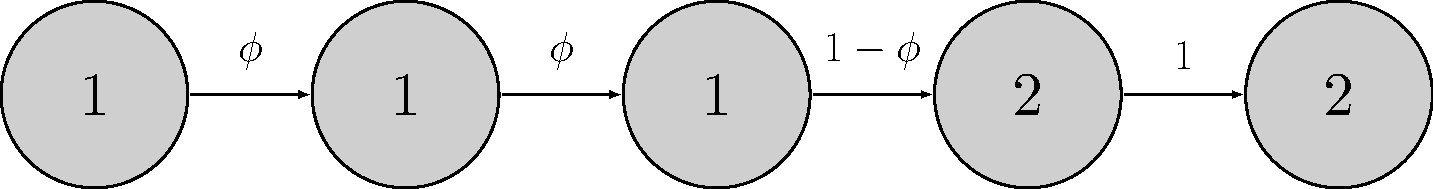
\includegraphics{banana-book_files/figure-latex/unnamed-chunk-111-1.pdf}

\hypertarget{what-if-covariates-vary-with-individual-and-time}{%
\subsection{What if covariates vary with individual and time?}\label{what-if-covariates-vary-with-individual-and-time}}

\hypertarget{age}{%
\subsubsection{Age}\label{age}}

Think of age for example (see exercises in Worksheets); covariate or nested indexing works fine.

Age in capture-recapture has a particular meaning in capture-recapture analyses. It is the time elapsed since first encounter, which is a proxy of true age obviously, but not true age. Of course, if age is known at first encounter, then it is the true age.

Another important remark is that age is an individual covariate, but in contrast with the wing length covariate we considered in the previous examples, age varies over time. The cool thing is that it has no missing value as age at \(t+1\) is just age at \(t\) to which we add 1. This suggests a way to code the age effect in nimble as follows.

\begin{Shaded}
\begin{Highlighting}[]
\NormalTok{hmm.phiage.in }\OtherTok{\textless{}{-}} \FunctionTok{nimbleCode}\NormalTok{(\{}
\NormalTok{  p }\SpecialCharTok{\textasciitilde{}} \FunctionTok{dunif}\NormalTok{(}\DecValTok{0}\NormalTok{, }\DecValTok{1}\NormalTok{) }\CommentTok{\# prior detection}
\NormalTok{  omega[}\DecValTok{1}\NormalTok{,}\DecValTok{1}\NormalTok{] }\OtherTok{\textless{}{-}} \DecValTok{1} \SpecialCharTok{{-}}\NormalTok{ p    }\CommentTok{\# Pr(alive t {-}\textgreater{} non{-}detected t)}
\NormalTok{  omega[}\DecValTok{1}\NormalTok{,}\DecValTok{2}\NormalTok{] }\OtherTok{\textless{}{-}}\NormalTok{ p        }\CommentTok{\# Pr(alive t {-}\textgreater{} detected t)}
\NormalTok{  omega[}\DecValTok{2}\NormalTok{,}\DecValTok{1}\NormalTok{] }\OtherTok{\textless{}{-}} \DecValTok{1}        \CommentTok{\# Pr(dead t {-}\textgreater{} non{-}detected t)}
\NormalTok{  omega[}\DecValTok{2}\NormalTok{,}\DecValTok{2}\NormalTok{] }\OtherTok{\textless{}{-}} \DecValTok{0}        \CommentTok{\# Pr(dead t {-}\textgreater{} detected t)}
  \ControlFlowTok{for}\NormalTok{ (i }\ControlFlowTok{in} \DecValTok{1}\SpecialCharTok{:}\NormalTok{N)\{}
    \ControlFlowTok{for}\NormalTok{ (t }\ControlFlowTok{in}\NormalTok{ first[i]}\SpecialCharTok{:}\NormalTok{(T}\DecValTok{{-}1}\NormalTok{))\{}
    \FunctionTok{logit}\NormalTok{(phi[i,t]) }\OtherTok{\textless{}{-}}\NormalTok{ beta[}\DecValTok{1}\NormalTok{] }\SpecialCharTok{+}\NormalTok{ beta[}\DecValTok{2}\NormalTok{] }\SpecialCharTok{*} \FunctionTok{equals}\NormalTok{(t, first[i]) }\CommentTok{\# phi1 = beta1 + beta2 and phi1+ = beta1}
\NormalTok{    gamma[}\DecValTok{1}\NormalTok{,}\DecValTok{1}\NormalTok{,i,t] }\OtherTok{\textless{}{-}}\NormalTok{ phi[i,t]      }\CommentTok{\# Pr(alive t {-}\textgreater{} alive t+1)}
\NormalTok{    gamma[}\DecValTok{1}\NormalTok{,}\DecValTok{2}\NormalTok{,i,t] }\OtherTok{\textless{}{-}} \DecValTok{1} \SpecialCharTok{{-}}\NormalTok{ phi[i,t]  }\CommentTok{\# Pr(alive t {-}\textgreater{} dead t+1)}
\NormalTok{    gamma[}\DecValTok{2}\NormalTok{,}\DecValTok{1}\NormalTok{,i,t] }\OtherTok{\textless{}{-}} \DecValTok{0}           \CommentTok{\# Pr(dead t {-}\textgreater{} alive t+1)}
\NormalTok{    gamma[}\DecValTok{2}\NormalTok{,}\DecValTok{2}\NormalTok{,i,t] }\OtherTok{\textless{}{-}} \DecValTok{1}           \CommentTok{\# Pr(dead t {-}\textgreater{} dead t+1)}
\NormalTok{    \}}
\NormalTok{  \}}
\NormalTok{  beta[}\DecValTok{1}\NormalTok{] }\SpecialCharTok{\textasciitilde{}} \FunctionTok{dnorm}\NormalTok{(}\AttributeTok{mean =} \DecValTok{0}\NormalTok{, }\AttributeTok{sd =} \FloatTok{1.5}\NormalTok{) }\CommentTok{\# phi1+}
\NormalTok{  beta[}\DecValTok{2}\NormalTok{] }\SpecialCharTok{\textasciitilde{}} \FunctionTok{dnorm}\NormalTok{(}\AttributeTok{mean =} \DecValTok{0}\NormalTok{, }\AttributeTok{sd =} \FloatTok{1.5}\NormalTok{) }\CommentTok{\# phi1 {-} phi1+}
\NormalTok{  phi1plus }\OtherTok{\textless{}{-}} \FunctionTok{plogis}\NormalTok{(beta[}\DecValTok{1}\NormalTok{])         }\CommentTok{\# phi1+}
\NormalTok{  phi1 }\OtherTok{\textless{}{-}} \FunctionTok{plogis}\NormalTok{(beta[}\DecValTok{1}\NormalTok{] }\SpecialCharTok{+}\NormalTok{ beta[}\DecValTok{2}\NormalTok{])   }\CommentTok{\# phi1}
\NormalTok{  delta[}\DecValTok{1}\NormalTok{] }\OtherTok{\textless{}{-}} \DecValTok{1}          \CommentTok{\# Pr(alive t = 1) = 1}
\NormalTok{  delta[}\DecValTok{2}\NormalTok{] }\OtherTok{\textless{}{-}} \DecValTok{0}          \CommentTok{\# Pr(dead t = 1) = 0}
  \CommentTok{\# likelihood}
  \ControlFlowTok{for}\NormalTok{ (i }\ControlFlowTok{in} \DecValTok{1}\SpecialCharTok{:}\NormalTok{N)\{}
\NormalTok{    z[i,first[i]] }\SpecialCharTok{\textasciitilde{}} \FunctionTok{dcat}\NormalTok{(delta[}\DecValTok{1}\SpecialCharTok{:}\DecValTok{2}\NormalTok{])}
    \ControlFlowTok{for}\NormalTok{ (j }\ControlFlowTok{in}\NormalTok{ (first[i]}\SpecialCharTok{+}\DecValTok{1}\NormalTok{)}\SpecialCharTok{:}\NormalTok{T)\{}
\NormalTok{      z[i,j] }\SpecialCharTok{\textasciitilde{}} \FunctionTok{dcat}\NormalTok{(gamma[z[i,j}\DecValTok{{-}1}\NormalTok{], }\DecValTok{1}\SpecialCharTok{:}\DecValTok{2}\NormalTok{, i, j}\DecValTok{{-}1}\NormalTok{])}
\NormalTok{      y[i,j] }\SpecialCharTok{\textasciitilde{}} \FunctionTok{dcat}\NormalTok{(omega[z[i,j], }\DecValTok{1}\SpecialCharTok{:}\DecValTok{2}\NormalTok{])}
\NormalTok{    \}}
\NormalTok{  \}}
\NormalTok{\})}
\end{Highlighting}
\end{Shaded}

Constants in a list.

\begin{Shaded}
\begin{Highlighting}[]
\NormalTok{first }\OtherTok{\textless{}{-}} \FunctionTok{apply}\NormalTok{(y, }\DecValTok{1}\NormalTok{, }\ControlFlowTok{function}\NormalTok{(x) }\FunctionTok{min}\NormalTok{(}\FunctionTok{which}\NormalTok{(x }\SpecialCharTok{!=}\DecValTok{0}\NormalTok{)))}
\NormalTok{my.constants }\OtherTok{\textless{}{-}} \FunctionTok{list}\NormalTok{(}\AttributeTok{N =} \FunctionTok{nrow}\NormalTok{(y), }
                     \AttributeTok{T =} \FunctionTok{ncol}\NormalTok{(y), }
                     \AttributeTok{first =}\NormalTok{ first)}
\end{Highlighting}
\end{Shaded}

Data in a list.

\begin{Shaded}
\begin{Highlighting}[]
\NormalTok{my.data }\OtherTok{\textless{}{-}} \FunctionTok{list}\NormalTok{(}\AttributeTok{y =}\NormalTok{ y }\SpecialCharTok{+} \DecValTok{1}\NormalTok{)}
\end{Highlighting}
\end{Shaded}

Initial values.

\begin{Shaded}
\begin{Highlighting}[]
\NormalTok{zinits }\OtherTok{\textless{}{-}}\NormalTok{ y}
\NormalTok{zinits[zinits }\SpecialCharTok{==} \DecValTok{0}\NormalTok{] }\OtherTok{\textless{}{-}} \DecValTok{1}
\NormalTok{initial.values }\OtherTok{\textless{}{-}} \ControlFlowTok{function}\NormalTok{() }\FunctionTok{list}\NormalTok{(}\AttributeTok{beta =} \FunctionTok{rnorm}\NormalTok{(}\DecValTok{2}\NormalTok{,}\DecValTok{0}\NormalTok{,}\DecValTok{5}\NormalTok{),}
                                  \AttributeTok{p =} \FunctionTok{runif}\NormalTok{(}\DecValTok{1}\NormalTok{,}\DecValTok{0}\NormalTok{,}\DecValTok{1}\NormalTok{),}
                                  \AttributeTok{z =}\NormalTok{ zinits)}
\end{Highlighting}
\end{Shaded}

Parameters to be monitored.

\begin{Shaded}
\begin{Highlighting}[]
\NormalTok{parameters.to.save }\OtherTok{\textless{}{-}} \FunctionTok{c}\NormalTok{(}\StringTok{"phi1"}\NormalTok{, }\StringTok{"phi1plus"}\NormalTok{, }\StringTok{"p"}\NormalTok{)}
\end{Highlighting}
\end{Shaded}

MCMC details.

\begin{Shaded}
\begin{Highlighting}[]
\NormalTok{n.iter }\OtherTok{\textless{}{-}} \DecValTok{5000}
\NormalTok{n.burnin }\OtherTok{\textless{}{-}} \DecValTok{2500}
\NormalTok{n.chains }\OtherTok{\textless{}{-}} \DecValTok{2}
\end{Highlighting}
\end{Shaded}

Run nimble.

\begin{Shaded}
\begin{Highlighting}[]
\NormalTok{mcmc.phi.age.in }\OtherTok{\textless{}{-}} \FunctionTok{nimbleMCMC}\NormalTok{(}\AttributeTok{code =}\NormalTok{ hmm.phiage.in, }
                             \AttributeTok{constants =}\NormalTok{ my.constants,}
                             \AttributeTok{data =}\NormalTok{ my.data,              }
                             \AttributeTok{inits =}\NormalTok{ initial.values,}
                             \AttributeTok{monitors =}\NormalTok{ parameters.to.save,}
                             \AttributeTok{niter =}\NormalTok{ n.iter,}
                             \AttributeTok{nburnin =}\NormalTok{ n.burnin, }
                             \AttributeTok{nchains =}\NormalTok{ n.chains)}
\end{Highlighting}
\end{Shaded}

Display results.

\begin{verbatim}
##          mean   sd 2.5%  50% 97.5% Rhat n.eff
## p        0.89 0.03 0.83 0.90  0.94 1.00   402
## phi1     0.56 0.03 0.49 0.55  0.63 1.01   689
## phi1plus 0.57 0.04 0.50 0.57  0.64 1.00   309
\end{verbatim}

Another method to include an age effect is to create an individual by time covariate and use nested indexing (as in the previous example) to distinguish survival after first detection from survival afterwards.

\begin{Shaded}
\begin{Highlighting}[]
\NormalTok{age }\OtherTok{\textless{}{-}} \FunctionTok{matrix}\NormalTok{(}\ConstantTok{NA}\NormalTok{, }\AttributeTok{nrow =} \FunctionTok{nrow}\NormalTok{(y), }\AttributeTok{ncol =} \FunctionTok{ncol}\NormalTok{(y) }\SpecialCharTok{{-}} \DecValTok{1}\NormalTok{)}
\ControlFlowTok{for}\NormalTok{ (i }\ControlFlowTok{in} \DecValTok{1}\SpecialCharTok{:}\FunctionTok{nrow}\NormalTok{(age))\{}
  \ControlFlowTok{for}\NormalTok{ (j }\ControlFlowTok{in} \DecValTok{1}\SpecialCharTok{:}\FunctionTok{ncol}\NormalTok{(age))\{}
    \ControlFlowTok{if}\NormalTok{ (j }\SpecialCharTok{==}\NormalTok{ first[i]) age[i,j] }\OtherTok{\textless{}{-}} \DecValTok{1}
    \ControlFlowTok{if}\NormalTok{ (j }\SpecialCharTok{\textgreater{}}\NormalTok{ first[i]) age[i,j] }\OtherTok{\textless{}{-}} \DecValTok{2}
\NormalTok{  \}}
\NormalTok{\}}
\end{Highlighting}
\end{Shaded}

The model. Careful, now survival is no longer defined on the logit scale as in the previous model, so we use uniform priors.

\begin{Shaded}
\begin{Highlighting}[]
\NormalTok{hmm.phiage.out }\OtherTok{\textless{}{-}} \FunctionTok{nimbleCode}\NormalTok{(\{}
\NormalTok{  p }\SpecialCharTok{\textasciitilde{}} \FunctionTok{dunif}\NormalTok{(}\DecValTok{0}\NormalTok{, }\DecValTok{1}\NormalTok{) }\CommentTok{\# prior detection}
\NormalTok{  omega[}\DecValTok{1}\NormalTok{,}\DecValTok{1}\NormalTok{] }\OtherTok{\textless{}{-}} \DecValTok{1} \SpecialCharTok{{-}}\NormalTok{ p    }\CommentTok{\# Pr(alive t {-}\textgreater{} non{-}detected t)}
\NormalTok{  omega[}\DecValTok{1}\NormalTok{,}\DecValTok{2}\NormalTok{] }\OtherTok{\textless{}{-}}\NormalTok{ p        }\CommentTok{\# Pr(alive t {-}\textgreater{} detected t)}
\NormalTok{  omega[}\DecValTok{2}\NormalTok{,}\DecValTok{1}\NormalTok{] }\OtherTok{\textless{}{-}} \DecValTok{1}        \CommentTok{\# Pr(dead t {-}\textgreater{} non{-}detected t)}
\NormalTok{  omega[}\DecValTok{2}\NormalTok{,}\DecValTok{2}\NormalTok{] }\OtherTok{\textless{}{-}} \DecValTok{0}        \CommentTok{\# Pr(dead t {-}\textgreater{} detected t)}
  \ControlFlowTok{for}\NormalTok{ (i }\ControlFlowTok{in} \DecValTok{1}\SpecialCharTok{:}\NormalTok{N)\{}
    \ControlFlowTok{for}\NormalTok{ (t }\ControlFlowTok{in}\NormalTok{ first[i]}\SpecialCharTok{:}\NormalTok{(T}\DecValTok{{-}1}\NormalTok{))\{}
\NormalTok{    phi[i,t] }\OtherTok{\textless{}{-}}\NormalTok{ beta[age[i,t]] }\CommentTok{\# beta1 = phi1, beta2 = phi1+}
\NormalTok{    gamma[}\DecValTok{1}\NormalTok{,}\DecValTok{1}\NormalTok{,i,t] }\OtherTok{\textless{}{-}}\NormalTok{ phi[i,t]      }\CommentTok{\# Pr(alive t {-}\textgreater{} alive t+1)}
\NormalTok{    gamma[}\DecValTok{1}\NormalTok{,}\DecValTok{2}\NormalTok{,i,t] }\OtherTok{\textless{}{-}} \DecValTok{1} \SpecialCharTok{{-}}\NormalTok{ phi[i,t]  }\CommentTok{\# Pr(alive t {-}\textgreater{} dead t+1)}
\NormalTok{    gamma[}\DecValTok{2}\NormalTok{,}\DecValTok{1}\NormalTok{,i,t] }\OtherTok{\textless{}{-}} \DecValTok{0}           \CommentTok{\# Pr(dead t {-}\textgreater{} alive t+1)}
\NormalTok{    gamma[}\DecValTok{2}\NormalTok{,}\DecValTok{2}\NormalTok{,i,t] }\OtherTok{\textless{}{-}} \DecValTok{1}           \CommentTok{\# Pr(dead t {-}\textgreater{} dead t+1)}
\NormalTok{    \}}
\NormalTok{  \}}
\NormalTok{  beta[}\DecValTok{1}\NormalTok{] }\SpecialCharTok{\textasciitilde{}} \FunctionTok{dunif}\NormalTok{(}\DecValTok{0}\NormalTok{, }\DecValTok{1}\NormalTok{) }\CommentTok{\# phi1}
\NormalTok{  beta[}\DecValTok{2}\NormalTok{] }\SpecialCharTok{\textasciitilde{}} \FunctionTok{dunif}\NormalTok{(}\DecValTok{0}\NormalTok{, }\DecValTok{1}\NormalTok{) }\CommentTok{\# phi1+}
\NormalTok{  phi1 }\OtherTok{\textless{}{-}}\NormalTok{ beta[}\DecValTok{1}\NormalTok{]}
\NormalTok{  phi1plus }\OtherTok{\textless{}{-}}\NormalTok{ beta[}\DecValTok{2}\NormalTok{]}
\NormalTok{  delta[}\DecValTok{1}\NormalTok{] }\OtherTok{\textless{}{-}} \DecValTok{1}          \CommentTok{\# Pr(alive t = 1) = 1}
\NormalTok{  delta[}\DecValTok{2}\NormalTok{] }\OtherTok{\textless{}{-}} \DecValTok{0}          \CommentTok{\# Pr(dead t = 1) = 0}
  \CommentTok{\# likelihood}
  \ControlFlowTok{for}\NormalTok{ (i }\ControlFlowTok{in} \DecValTok{1}\SpecialCharTok{:}\NormalTok{N)\{}
\NormalTok{    z[i,first[i]] }\SpecialCharTok{\textasciitilde{}} \FunctionTok{dcat}\NormalTok{(delta[}\DecValTok{1}\SpecialCharTok{:}\DecValTok{2}\NormalTok{])}
    \ControlFlowTok{for}\NormalTok{ (j }\ControlFlowTok{in}\NormalTok{ (first[i]}\SpecialCharTok{+}\DecValTok{1}\NormalTok{)}\SpecialCharTok{:}\NormalTok{T)\{}
\NormalTok{      z[i,j] }\SpecialCharTok{\textasciitilde{}} \FunctionTok{dcat}\NormalTok{(gamma[z[i,j}\DecValTok{{-}1}\NormalTok{], }\DecValTok{1}\SpecialCharTok{:}\DecValTok{2}\NormalTok{, i, j}\DecValTok{{-}1}\NormalTok{])}
\NormalTok{      y[i,j] }\SpecialCharTok{\textasciitilde{}} \FunctionTok{dcat}\NormalTok{(omega[z[i,j], }\DecValTok{1}\SpecialCharTok{:}\DecValTok{2}\NormalTok{])}
\NormalTok{    \}}
\NormalTok{  \}}
\NormalTok{\})}
\end{Highlighting}
\end{Shaded}

Constants in a list, inculding the age matrix covariate.

\begin{Shaded}
\begin{Highlighting}[]
\NormalTok{first }\OtherTok{\textless{}{-}} \FunctionTok{apply}\NormalTok{(y, }\DecValTok{1}\NormalTok{, }\ControlFlowTok{function}\NormalTok{(x) }\FunctionTok{min}\NormalTok{(}\FunctionTok{which}\NormalTok{(x }\SpecialCharTok{!=}\DecValTok{0}\NormalTok{)))}
\NormalTok{my.constants }\OtherTok{\textless{}{-}} \FunctionTok{list}\NormalTok{(}\AttributeTok{N =} \FunctionTok{nrow}\NormalTok{(y), }
                     \AttributeTok{T =} \FunctionTok{ncol}\NormalTok{(y), }
                     \AttributeTok{first =}\NormalTok{ first,}
                     \AttributeTok{age =}\NormalTok{ age)}
\end{Highlighting}
\end{Shaded}

Data in a list.

\begin{Shaded}
\begin{Highlighting}[]
\NormalTok{my.data }\OtherTok{\textless{}{-}} \FunctionTok{list}\NormalTok{(}\AttributeTok{y =}\NormalTok{ y }\SpecialCharTok{+} \DecValTok{1}\NormalTok{)}
\end{Highlighting}
\end{Shaded}

Initial values.

\begin{Shaded}
\begin{Highlighting}[]
\NormalTok{zinits }\OtherTok{\textless{}{-}}\NormalTok{ y}
\NormalTok{zinits[zinits }\SpecialCharTok{==} \DecValTok{0}\NormalTok{] }\OtherTok{\textless{}{-}} \DecValTok{1}
\NormalTok{initial.values }\OtherTok{\textless{}{-}} \ControlFlowTok{function}\NormalTok{() }\FunctionTok{list}\NormalTok{(}\AttributeTok{beta =} \FunctionTok{runif}\NormalTok{(}\DecValTok{2}\NormalTok{,}\DecValTok{0}\NormalTok{,}\DecValTok{1}\NormalTok{),}
                                  \AttributeTok{p =} \FunctionTok{runif}\NormalTok{(}\DecValTok{1}\NormalTok{,}\DecValTok{0}\NormalTok{,}\DecValTok{1}\NormalTok{),}
                                  \AttributeTok{z =}\NormalTok{ zinits)}
\end{Highlighting}
\end{Shaded}

Parameters to be monitored.

\begin{Shaded}
\begin{Highlighting}[]
\NormalTok{parameters.to.save }\OtherTok{\textless{}{-}} \FunctionTok{c}\NormalTok{(}\StringTok{"phi1"}\NormalTok{, }\StringTok{"phi1plus"}\NormalTok{, }\StringTok{"p"}\NormalTok{)}
\end{Highlighting}
\end{Shaded}

MCMC details.

\begin{Shaded}
\begin{Highlighting}[]
\NormalTok{n.iter }\OtherTok{\textless{}{-}} \DecValTok{5000}
\NormalTok{n.burnin }\OtherTok{\textless{}{-}} \DecValTok{2500}
\NormalTok{n.chains }\OtherTok{\textless{}{-}} \DecValTok{2}
\end{Highlighting}
\end{Shaded}

Run nimble.

\begin{Shaded}
\begin{Highlighting}[]
\NormalTok{mcmc.phi.age.out }\OtherTok{\textless{}{-}} \FunctionTok{nimbleMCMC}\NormalTok{(}\AttributeTok{code =}\NormalTok{ hmm.phiage.out, }
                               \AttributeTok{constants =}\NormalTok{ my.constants,}
                               \AttributeTok{data =}\NormalTok{ my.data,              }
                               \AttributeTok{inits =}\NormalTok{ initial.values,}
                               \AttributeTok{monitors =}\NormalTok{ parameters.to.save,}
                               \AttributeTok{niter =}\NormalTok{ n.iter,}
                               \AttributeTok{nburnin =}\NormalTok{ n.burnin, }
                               \AttributeTok{nchains =}\NormalTok{ n.chains)}
\end{Highlighting}
\end{Shaded}

Display results.

\begin{Shaded}
\begin{Highlighting}[]
\FunctionTok{load}\NormalTok{(here}\SpecialCharTok{::}\FunctionTok{here}\NormalTok{(}\StringTok{"dat/phiageout.RData"}\NormalTok{))}
\FunctionTok{MCMCsummary}\NormalTok{(mcmc.phi.age.out, }\AttributeTok{round =} \DecValTok{2}\NormalTok{)}
\DocumentationTok{\#\#          mean   sd 2.5\%  50\% 97.5\% Rhat n.eff}
\DocumentationTok{\#\# p        0.90 0.03 0.84 0.90  0.95 1.02   438}
\DocumentationTok{\#\# phi1     0.55 0.03 0.48 0.55  0.62 1.00   878}
\DocumentationTok{\#\# phi1plus 0.57 0.04 0.50 0.57  0.64 1.02  1048}
\end{Highlighting}
\end{Shaded}

\hypertarget{trap-dependence}{%
\subsubsection{Trap-dependence}\label{trap-dependence}}

Add example for trap-dependence w/ time individual covariate. Move it to case study w/ multievent.

\hypertarget{missing-values}{%
\subsubsection{Missing values}\label{missing-values}}

Now, think of body size across life. Problem is we cannot record size when animal is non-detected. Discretize in small, medium and large and treat as a state. More later. Assume a model for covariate and fill in missing values (imputation).

\hypertarget{summary}{%
\section{Summary}\label{summary}}

\begin{itemize}
\item
  Statistical models rely on assumptions, and the CJS model makes no exception.
\item
  Blabla.
\end{itemize}

\hypertarget{suggested-reading}{%
\section{Suggested reading}\label{suggested-reading}}

\begin{itemize}
\item
  A bit of history about the CJS model and the people involved in its developements by \href{https://research-repository.st-andrews.ac.uk/handle/10023/8869}{S.T. Buckland (2016)}.
\item
  Mettre papier Vlad et Morten pour temps, et mon papier Oikos pour individu.
\item
  CJS state-space formulation \href{https://oliviergimenez.github.io/pubs/Gimenezetal2007EcologicalModelling.pdf}{Gimenez et al.~(2007)} and \href{https://onlinelibrary.wiley.com/doi/10.1111/j.1541-0420.2007.00891.x}{Royle (2008)}.
\item
  Also read Lebreton et al.~1992, long monography, but a gem, w/ introduction to AIC, model assumptions, etc.
\item
  About WAIC, more in this video \url{https://www.youtube.com/watch?v=vSjL2Zc-gEQ} by R. McElreath. Cite relevant papers in particular paper by Gelman et al.~2014 Understanding predictive information criteria for Bayesian models.
\item
  Work on missing values by \href{https://onlinelibrary.wiley.com/doi/abs/10.1111/j.1541-0420.2005.00399.x}{Bonner et al.~(2006)} and \href{https://projecteuclid.org/journals/annals-of-applied-statistics/volume-7/issue-3/Maximum-likelihood-estimation-of-markrecapturerecovery-models-in-the-presence-of/10.1214/13-AOAS644.full}{Langrock and King (2013)} and \href{https://link.springer.com/article/10.1007/s13253-014-0184-z}{Worthington et al.~(2015)}.
\item
  The example on how to incorporate prior information is in \href{https://besjournals.onlinelibrary.wiley.com/doi/abs/10.1111/j.1365-2664.2005.01101.x}{McCarthy and Masters (2005)}.
\item
  On posterior predictive check, see paper by Chambert \url{https://doi.org/10.1002/ece3.993}, or Conn \url{https://doi.org/10.1002/ecm.1314}.
\item
  Combine live recapture w/ dead recoveries by \href{https://www.tandfonline.com/doi/pdf/10.1080/00063659909477230}{Lebreton et al.~(1999)} and go spatial to account for emigration \href{https://esajournals.onlinelibrary.wiley.com/doi/full/10.1890/12-0124.1}{Gilroy et al.~(2012)} and \href{https://besjournals.onlinelibrary.wiley.com/doi/full/10.1111/2041-210X.12134}{Schaub \& Royle (2014)}.
\item
  Non-identifiability in a Bayesian framework, see \href{https://oliviergimenez.github.io/pubs/Gimenezetal2009-weakidentifiability.pdf}{Gimenez et al.~(2009)} and \href{https://www.routledge.com/Parameter-Redundancy-and-Identifiability/Cole/p/book/9781498720878}{book by Cole (2020)}.
\end{itemize}

\hypertarget{part-iii.-case-studies}{%
\part{III. Case studies}\label{part-iii.-case-studies}}

\hypertarget{introduction-3}{%
\chapter*{Introduction}\label{introduction-3}}


\hypertarget{part-iv.-conclusions}{%
\part{IV. Conclusions}\label{part-iv.-conclusions}}

\hypertarget{introduction-4}{%
\chapter*{Introduction}\label{introduction-4}}


\hypertarget{take-home-messages}{%
\chapter*{Take-home messages}\label{take-home-messages}}


--\textgreater{}
--\textgreater{}

--\textgreater{}

--\textgreater{}

--\textgreater{}

\backmatter

  \bibliography{book.bib}

\printindex

\end{document}
